\chapter{Quantum Perceptron}

Intelligent machines are as old as Greek mythology. In \textit{The Argonautica}, the bronze automaton Talos wards the island of Crete to protect it from the troublesome Argonauts, who seek to steal the Golden Fleece \cite{Seaton1912}. Although we are still far away from animating metal statues, substantial progress has been made with regards to simulating intelligence that does not require a divine touch. One of the striking properties of human cognition is the ability to process complex sensory data, such as vision or sound. This ability stems from the fact that the brain is able to filter redundant information, and extract useful details that are required for human functioning. This mechanism of information extraction is what we try to replicate in the field of artificial intelligence (AI). The problem is that nature has refined this mechanism through billions of years of trial-and-error, with a myriad individuals trying to adapt to their surroundings, optimizing the cost function that is survival. Even with modern computers we cannot hope to simulate this whole process. What we can learn from nature is that a computational model that generalizes from experience is powerful. The question becomes: what does this model look like? \newline

\noindent The field of AI originated from computing science, with Alan Turing first speculating about the possibility of building intelligent machines using digital computers in a 1950 paper. In this seminal work, he explored early ideas of machine learning, genetic algorithms and reinforcement learning \cite{Turing1950}. Soon thereafter, two MIT scientists embraced Hebb's neuroscientific theory that "Cells that fire together, wire together" \cite{Hebb1949}, and built a neural net consisting of 40 Hebbian synapses from analogue electronics. A few years later, Rosenblatt's perceptron received a lot of attention for its ability to learn any problem that could be separated linearly \cite{Rosenblatt1958}. In general, there was a lot of optimism in the 1950s and 1960s about the future of AI, but problems that plagued the field from the beginning were becoming more troublesome. In those early days, most AI approaches were symbolic and rule-based in nature, which did not scale well to larger of more complex systems. Limited generalization abilities, a combinatoric explosion of the state space and intractable calculations stumped progress, and led governments to cut funding for most of the research throughout the 1970s. Additionally, the infant industry around machine learning never bloomed, as companies failed to fulfill exuberant promises. The field entered a period which has received the dramatic name ``AI winter", where progress was slow. Parallel to the symbolic approach to AI, the field of machine learning focused on more statistical approach to intelligence. The language of machine learning is one of linear algebra, optimization and statistics;  fields of study that developed rapidly after the axiomization of mathematics in the early 1900s. When the shortcomings of the symbolic AI became apparent, it allowed machine learning to rise to prominence. In the mid 1980s several groups rediscovered the method of automatic differentiation which allowed for easy calculation of gradients by backpropagation. This paved the way for training multilayer networks that could replace hand engineered features with more abstract representations. In 1984 Valiant proposed to study what computers can learn instead of what they can calculate, laying the foundation for the field of computational learning theory \cite{Valiant1984}. Along with this development, connections between statistical physics and machine learning were made, which finally shifted the field from arule-based approach to a more statistical paradigm \cite{Carleo2019}. A thaw had set in, and the 1990s and 2000s saw the development of many different algorithms: support vector machines, Recurrent Neural Networks, Random Forests and Hidden Markov models to name a few \cite{LeCun1998, Russell2003}. Due to the successes of these techniques machine learning permeated into scientific fields as bioinformatics \cite{Larranaga2006}, medical imaging \cite{Chartrand2017}, astrophysics \cite{Collister2004} and particle physics \cite{Radovic2018}. In the 2010s, catalyzed by the availability of large data sets and cheap parallel processing power in the form of GPU's, neural networks with a large amount of layers (deep learning) could be trained successfully. This has led to numerous successes, from beating the best Go player \cite{Silver2016}, real-time language translation from video \cite{GoogleTranslate} and improved autonomous driving \cite{Ouyang2013, Zhu2016}. Although simulating intelligent life is probably still far away, machine learning has been applied very successfully to specific tasks for which data was abundant and its impact on society has been significant.

\section{Quantum Machine Learning}

A model agnostic approach to understanding nature probably does not sit well with most physicists, but the potential of machine learning for physics cannot be ignored. The fusion of machine learning with quantum mechanics is called quantum machine learning and shows great promise \cite{Biamonte2017}. The usage of the term quantum machine learning is a bit ambiguous, since it is used to describe different types of research. The relations between these types of research are depicted schematically in figure \ref{fig:qml_field}.\newline

\noindent Inspired by the success of fusing physics with machine learning we focus on a relatively unexplored area of this research: learning machine learning models for classical data using quantum cost functions. The perceptron is of particular interest, since it serves as the building block for neural networks and deep learning \cite{LeCun2015}. Some work has been done to develop quantum equivalents of neural networks, but these proposals only use quantum effects in the nodes or synapses of the network. They are still trained by minimizing a classical cost function \cite{Zhou1999, Kouda2005, Zhou2007, Altaisky2013, Xuan2011, Shang2015, Schuld2014, Jeswal2018}. Constructing quantum probabilistic models from density matrices is a new direction of quantum machine learning research \cite{Amin2018, Kappen2018}, where one exploits quantum effects in both the model and training procedure, by constructing a differentiable cost function in terms of density matrices. In this work, we use this approach to construct a quantum perceptron that uses a generalization of the classical likelihood function for learning, replacing the classical perceptron bit with a qubit. Others have attempted to generalize probability theory to density matrices, but the equivalent of conditional probabilities, conditional density matrices, do not preserve positive definiteness so states can be assigned a negative probability \cite{Cerf1999, Warmuth2006}. Our approach bypasses this difficulty because we construct a data density matrix from the probability amplitude of the empirical data distribution, which is always positive semidefinite. \newline

\noindent The proposed quantum-inspired perceptron allows us to better capture noisiness in data sets than a classical perceptron. Additionally, we show that by considering entangled qubits we can learn non-trivial separation boundaries, such as XOR. The model can easily be expanded to learn different types of data and provides a solid foundation to investigate other physically-inspired models. The most important results of this thesis are summarized in a 2019 paper \cite{Wiersema2019}. In chapter 2, we present a full analysis of the proposed model. Appendix \ref{sec:qm} contains background information for quantum physics, and will be referred to on occasion. The additional appendices contain lengthy calculations that were required for the analysis. For a detailed overview of quantum computing, which is briefly touched upon in the final section, the reader is referred to \cite{Nielsen2011}. For an excellent reference on machine learning, consider \cite{Murphy2012}.

\begin{figure}[htb!]
    \centering
    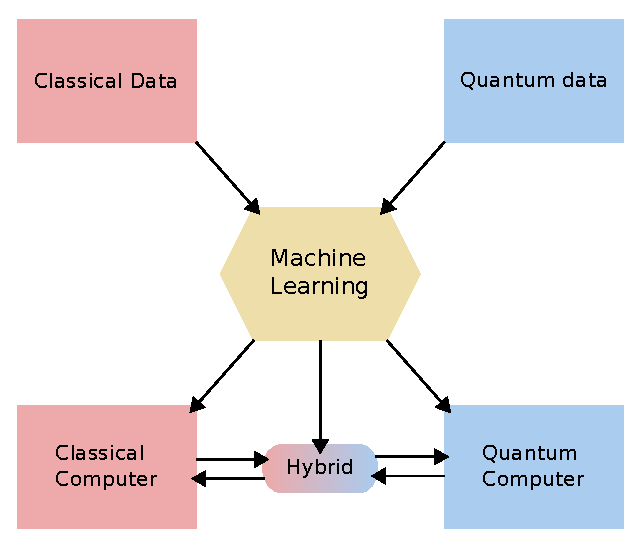
\includegraphics[width=0.6\textwidth]{figures/chapter1/overlap.eps}
    \caption{Overview of the field of quantum machine learning. A classical computer is defined as a von Neumann architecture computer. A quantum computer is either a Noisy Intermediate-Scale Quantum Computer or a quantum annealer. The difference between classical data and quantum data is that the source of quantum data is either some complex model of a quantum system, or experimental measures of a physical system. \textbf{Classical data $\to$ Classical computer:} The traditional field of machine learning, as previously discussed. \textbf{Quantum data $\to$ Classical computer:} This field is for instance concerned with understanding quantum many body interactions \cite{Carleo2017, Saito2018} through neural network states, providing speedups for Density Field Theory approaches \cite{Jacobsen2018, Hegde2017} or learning phase transitions in condensed matter systems \cite{Carrasquilla2017}. \textbf{Classical data $\to$ Quantum computer:} Here, classical data is encoded onto a quantum computer, and a quantum computing equivalent of a classical machine learning algorithm is used for learning \cite{Neven2018, Schuld2019a}. Another approach is to provide speedups for the underlying linear algebra routines \cite{Lloyd2009, Lloyd2013, Lloyd2014}. However, most of these proposals remain unfeasible due to the current limitations of modern quantum computers, which still lack long qubit coherence times and high gate fidelity \cite{Preskill2018}. \textbf{Quantum data $\to$ Quantum computer:} In quantum state tomography the goal is to reconstruct the density matrix of an unknown quantum state, through experimental measurement. The amount of measurements required can be large and machine learning can assist in reducing this cost \cite{Gross2010}.
    \textbf{Quantum kernel hybrid:} With quantum kernels one computes a classically intractable kernel function on a quantum computer, which is fed back to a classical computer and incoporated into a classical machine learning model \cite{Schuld2019a}.
    \textbf{Quantum-inspired hybrid:} Quantum-inspired algorithms are a hybrid, where classical data is used, but a quantum model is learned \cite{Biamonte2017, Stoudemire2016, Xie2017, Yang2004, Amin2018}. This is without involvement of a quantum computer and it is where the work of this thesis is located. The work in this thesis falls in the category \textbf{Hybrid}, since we use a quantum-inspired model but execute it on a classical computer.
    }
    \label{fig:qml_field}
\end{figure}
\clearpage
\section{Code}

The code used for this research initially contained only a model with the exact gradient update rules written in Python. When the models expanded to continuous, multiclass and entangled learning all the code was rewritten in a single big TensorFlow class. The reason for this is that for larger density matrices we have to rely on the numerical evaluation of the eigenvectors, which can be sped up significantly if performed in parallel on the GPU.\newline

TensorFlow is a high level graphical computing framework for Python that is optimized for GPU usage. It is maintained by Google and used by many authors in the machine learning community. Complicated models can easily be trained through the process of automatic differentiation, where the entire optimization schedule is decomposed in terms of simple mathematical operations so that gradients can be computed efficiently with the chain rule. The code with the TensorFlow model and ways to reproduce the most important figures in this thesis can be found on GitHub \cite{WiersemaGit2019a}. 

\section{Machine Learning}

Machine learning can be defined as a set of methods that can automatically detect patterns in data, and then uses these uncovered patterns to predict future data. Supervised learning is a subset of machine learning where we try to find a mapping $y = f(\mathbf{x})$ for data $\mathcal{D}\{(y, \mathbf{x})\}^N$. The input vector $\mathbf{x}$ is often called the feature vector and the output $y$ is called the label or response variable. In the case that $y$ is some real-valued scalar $y\in \mathbb{R}$ we talk about regression. If the output $y$ is from some finite set $C\in \{1,...,p\}$ we talk about classification, which is what we will consider from now on. Because data is often noisy, we make use of probability theory as an underlying framework for machine learning. The function $f(\mathbf{x})$ is then replaced by a conditional probability distribution $p(y | \mathbf{x}, \mathcal{D})$. Let us establish a couple of basic definitions from probability theory that will allow us to proceed with describing machine learning models.\newline

\noindent In machine learning we often deal with probability distributions over multiple random variables. A joint probability over random variables $X$, $Y$ is defined as 
    \begin{equation*}
        p(X,Y) = p(X|Y)p(Y),
    \end{equation*}
where  $p(X|Y)$ is the conditional probability that $X$ is true given that $Y$ is true. This also defines a conditional probability as 
\begin{equation*}
    p(X|Y) = \frac{p(X,Y) }{p(Y)}.
\end{equation*}
The marginal is obtained by summing out the random variables that are not of interest,
    \begin{equation*}
        p(X) = \sum_y p(X|Y=y)p(Y=y).
    \end{equation*}
Combining these definitions gives us Bayes' Rule,
    \begin{equation*}
        p(X|Y) = \frac{p(Y|X)p(X) }{p(Y)}.
    \end{equation*}
To not obfuscate everything with excessive notation we use the convention that for some data set $\mathcal{D} = \{(\mathbf{x}, y)\}^N$ the sum $\sum_\mathbf{x}$ is the sum over all the samples and $\sum_y$ is the sum over the possible labels for that sample. The sum over the tuple $\sum_{(\mathbf{x}, y)}$ indicates the sum over the sample, with its corresponding label in the data set $\mathcal{D}$.

\section{Classical Perceptron}\label{sec:cl_percp}

For supervised learning we are interested in inferring a function $f(\mathbf{x})$ that correctly predicts the output data $y$ for all samples $\mathbf{x} \in \mathbb{R}^d$ in the data. The classical perceptron is such a supervised learning model. It is a classifier that takes a set of linear predictors $h(\mathbf{x}) = \mathbf{w}\cdot \mathbf{x}$ and produces an output $y\in\{1,-1\}$. Perceptrons are important, because they form the building blocks of Multilayer Neural Networks (MLP) which are the driving force behind deep learning \cite{LeCun2015}.\newline

\noindent The most basic perceptron is Rosenblatt's perceptron, which was briefly mentioned in the introduction. This model generates an output by applying a nonlinear activation function $f(x) = \text{sgn}(x)$ to a linear predictor of the input data \cite{Rosenblatt1958}. The sign function $\text{sgn}(x)$ is defined as
\begin{equation*}
   \text{sgn(x)}=\begin{cases}
    -1 & \text{if $x<0$}\\
    0 & \text{if $x=0$}\\
     1 & \text{if $x>0$}
   \end{cases}.
\end{equation*}
In order to find the weights $\mathbf{w}$ that provide the optimal split of the data we use a simple learning rule. For the classical perceptron this learning rule is given by
\begin{align}
    \Delta \mathbf{w} = \epsilon (y - \text{sgn}(\mathbf{w}\cdot \mathbf{x})) \mathbf{x}, \label{eq:rosenblatt}
\end{align}
where $\epsilon$ is the learning rate. Geometrically the perceptron can be interpreted as an algorithm that tries to split the input space in two parts for $y=\{+1,-1\}$. When possible, the learning algorithm converges to a solution that separates the data perfectly. We then call the data linearly separable. We can add biases $w_0$ to the input to shift the activation function,
\begin{align*}
    \mathbf{w}\cdot\mathbf{x} = w_0 + \mathbf{w}\cdot\mathbf{x}  = w_0 + \sum_i w_ix_i^\mu,
\end{align*}
where $p$ is the number of inputs. Adding a bias provides an extra degree of freedom that allows the algorithm to deal with data that can not be separated with a line through the origin. This is shown schematically in figure \ref{fig:bias}. 
\begin{figure}[htb!]
    \centering
    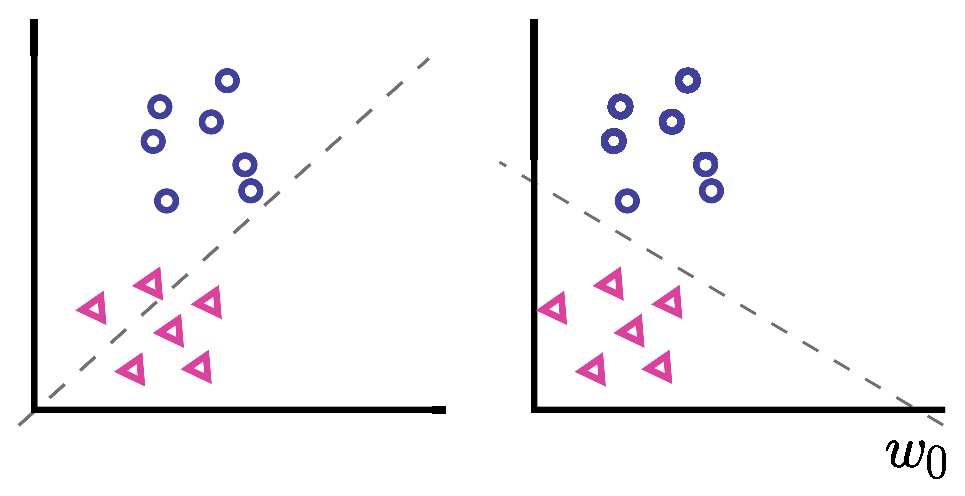
\includegraphics[width=\textwidth]{figures/chapter3/bias.eps}
    \caption{Schematic representation of separation boundaries through the input space. Adding a bias allows for easier learning because we are not restricted to slices through the feature space which go through the origin. }
    \label{fig:bias}
\end{figure}

\noindent Also, a translation $\mathbf{x}\rightarrow \mathbf{x} - \mathbf{x}^\prime$ of the data can be absorbed in the bias,
\begin{align}
    h^k &= \vecwk{k}\cdot (\mathbf{x} - \mathbf{x}^\prime)= \vecwk{k} \cdot \mathbf{x} - \overbrace{\vecwk{k}\cdot\mathbf{x}^\prime + w_0}^{w_0^\prime} \nonumber\\
    & = \mathbf{w}\cdot\mathbf{x} - w_0^\prime \label{eq:transl_inv}.
\end{align}
It has been shown that stacks of connected perceptrons, also known as neural networks, can in principle approximate any possible function \cite{Cybenko1989}. This implies that any mapping from data to label can be learned. The difficulty is in coming up with a learning procedure and network architecture that finds this universal approximator, and does not get stuck in suboptimal local minima. \newline

\noindent The activation function is a key part of the perceptron model. In Rosenblatt's perceptron the step function is proposed \textit{ad hoc} to mimic behaviour the behaviour of biological neurons. In the last two decades, research into neural networks has spawned a number of activation functions that attempt to either improve generalization properties of a network or hope to increase training speed \cite{Glorot15, Clevert2015, Hochreiter1998}. Another method for improving performance is choosing a suitable a cost function $E(x)$. This function attributes a cost to some event. For instance, by calculating the euclidean distance between the predicted label and the true label. If $E(x)$  is continuous and differentiable we can use gradient descent to find a local (under convexity global) minimum of that function. By making some assumptions about how the data is distributed, we can come up with an optimization criterion that is derived from a probabilistic model. An example of a model that uses such a criterion is logistic regression.

\section{Logistic Regression \label{sec:inference}}

In order to learn a statistical model we need come up with a model distribution $p(\mathcal{D} |\bm{\theta})$ of the data $\mathcal{D}$  given some parameters $\bm{\theta}$. This distribution is called the likelihood, it describes how likely the model is given the data and the parameters that we have chosen. In order to estimate the parameters of a statistical model we can use the technique of Maximum Likelihood Estimation. \newline 

\noindent Consider a probability density $p(\mathbf{x},y; \bm{\theta})$. For a fixed data set $\mathcal{D} = \{(\mathbf{x},y)\}^N$ the likelihood function describes the probability of the data given the model and some set of parameters $\bm{\theta}$, written as
\begin{equation}
    \mathcal{L} = p(\mathcal{D};\bm{\theta}).
\end{equation}
If the data independent and identically distributed (i.i.d.) then we can write the likelihood as the product of individual probabilities,
\begin{equation}
    \mathcal{L} = \prod_{(\mathbf{x},y)} p(\mathbf{x}, y|\bm{\theta}).
\end{equation}
By maximizing this likelihood, we can find the optimal set of parameters $\bm{\theta}$ that assigns the highest total probability of the data under the model probability density $p(\mathbf{x},y;\bm{\theta})$ \cite{Murphy2012}.
To ensure that we can properly calculate the total probability, we often minimize the negative log-likelihood instead, since the log-transformed function preserves the maximum but replaces the product by a sum. We will continue with the negative log-likelihood,
\begin{equation}
    \mathcal{L} = -\sum_{(\mathbf{x}, y)}\log( p(\mathbf{x},y; \bm{\theta})).
\end{equation}
Using the law of large numbers we can write 
\begin{align*}
    &\lim\limits_{N\to \infty} -\sum_{(\mathbf{x},y)} \log( p(\mathbf{x},y; \bm{\theta})) \rightarrow -\mathbb{E}\left[\log( p(y|\mathbf{x},\bm{\theta})) \right]_{ q(\mathbf{x},y)}\\
    &= -\sum_{\mathbf{x},y} q(\mathbf{x},y) \log( p(\mathbf{x},y;\bm{\theta}))\\
    &= -\sum_{\mathbf{x},y} q(\mathbf{x}) q(y|\mathbf{x})\log( p(y|\mathbf{x} ;\bm{\theta})) - q(\mathbf{x})\underbrace{q(y|\mathbf{x})}_{=1}\log(p(\mathbf{x};\bm{\theta}))\\
    &= -\sum_{\mathbf{x}} q(\mathbf{x}) \sum_y q(y|\mathbf{x})\log( p(y|\mathbf{x} ;\bm{\theta})) - q(\mathbf{x})\log(p(\mathbf{x};\bm{\theta}))\\
    & = \sum_{\mathbf{x}} q(\mathbf{x}) H(q(y|\mathbf{x};\bm{\theta}),p(y|\mathbf{x};\bm{\theta}))- q(\mathbf{x})\log(p(\mathbf{x};\bm{\theta})),
\end{align*}
where $ q(\mathbf{x},y)$ is the empirical distribution given by the data. The term
\begin{equation}
    H(q(y|\mathbf{x};\bm{\theta}),p(y|\mathbf{x};\bm{\theta})),
\end{equation} 
is known as the cross entropy and is a measure of ``distance" between two distributions. Notice that if we assume $p(\mathbf{x};\bm{\theta})=p(\mathbf{x})$ independent of $\bm{\theta}$ then when only have to calculate the cross entropy term, since the final term is constant with respect to the parameters of the model. \newline 

\noindent We can now construct a perceptron model, a binary classifier, analogous to Rosenblatt's perceptron as a probabilistic model with a binary response variable $y\in \{0,1\}$. For a random process with a binary random variable we can use a binomial regression model, which has probability density function is given by
\begin{equation*}
    \text{Bin}(k|n, \mu) = {n \choose k} \mu^k (1-\mu)^{n-k},
\end{equation*}
where we observe $k$ times label $y=1$ out of $n$ tries and $\mu\in[0,1]$ is the probability of finding $y=1$. If $n=1$, then
\begin{equation*}
    p(y|\bm{\theta}) = \text{Bin}(k|1,\bm{\theta})\rightarrow \text{Ber}(y|\bm{\theta})=\mu^{\mathbb{I}(y=1)} (1-\mu)^{\mathbb{I}(y=0)}.
\end{equation*}
In other words, for a single trial the variable is Bernoulli distributed. Assume that the distribution of labels also depends on the input $\mathbf{x}$. Then we can write the negative log-likelihood as
\begin{align*}
    \mathcal{L} &= - \sum_\mathbf{x} \log(\mu(\mathbf{x}; \theta)^{\mathbb{I}(y=1)} (1-\mu(\mathbf{x}; \theta))^{\mathbb{I}(y=0)})\\
    &=- \sum_\mathbf{x} y \log(\mu(\mathbf{x}; \theta)) + (1 - y) \log(1 - \mu(\mathbf{x}; \theta)).
\end{align*}
We further require that $\mu(\mathbf{x}; \theta)$ is a function of the linear predictor  $h(\mathbf{x}) = \mathbf{w} \cdot \mathbf{x}$, omitting the argument of $h$ for now. To ensure that $\mu(\mathbf{x}; \mathbf{w})$ is contained in $[0,1]$ we can assume that the errors are distributed according to the logistic distribution, given by the sigmoid function,
\begin{align}
    \mu(\mathbf{x}; \mathbf{w}) \equiv S(h(\mathbf{x})) &= \frac{1}{1 + e^{-h(\mathbf{x})}} = \frac{e^{h(\mathbf{x})/2}}{e^{h(\mathbf{x})/2} + e^{-h(\mathbf{x})/2}} = \frac{2e^{h(\mathbf{x})/2}}{\cosh(h(\mathbf{x})/2)}\label{eq:log_reg}\\
    1 - S(h(\mathbf{x})) &= \frac{2e^{-h(\mathbf{x})/2}}{\cosh(h(\mathbf{x})/2)}\nonumber.
\end{align}
which is the continuous extension of the step function with a codomain $(0,1)$, as can be seen in figure \ref{fig:sigmoid}. This model is called logistic regression. Now, if we take the perceptron of section \ref{sec:cl_percp} with a sigmoid activation as nonlinear function, we end up with logistic regression, but without the probabilistic motivation. Logistic regression is also equivalent to the probability distribution of an Ising spin at finite temperature under the Boltzmann distribution. If we rescale the output $y$, from $\{0,1\}\rightarrow\{-1,1\}$, then we can write the negative log-likelihood as
\begin{align*}
    \mathcal{L} &= - \sum_{\mathbf{x},y} \log(\frac{2e^{y h(\mathbf{x})/2}}{\cosh(h(\mathbf{x})/2)}),
\end{align*}
which under the distribution $q(\mathbf{x},y)$ of the data becomes
\begin{align}
    =  -\sum_{\mathbf{x}} q(\mathbf{x}) \sum_y q(y|\mathbf{x}) \log(\frac{e^{y h(\mathbf{x})/2}}{2 \cosh(h(\mathbf{x})/2)})  \label{eq:nll}.
\end{align}
\begin{figure}
    \centering
    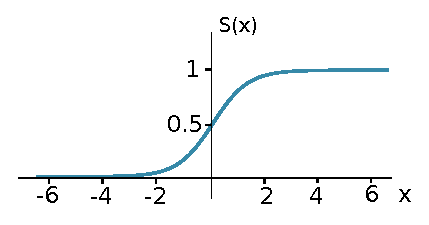
\includegraphics[width=\textwidth]{figures/chapter3/sigmoid.eps}
    \caption{The sigmoid function. $S(x)$ has codomain (0,1). For $x\approx4.5$ this gives $S(4.5) = 0.99$  which is already close to 1. Adding an inverse temperature $S(\beta x)$ allows for tuning of the smoothness of the function. In the limit $\beta \to \infty$ the sigmoid become a step function.}
    \label{fig:sigmoid}
\end{figure}

\noindent The nice thing about this formulation is that it gives us an optimization criterion motivated by probability theory, the negative log-likelihood. If we find the global minimum of this function we will have found the optimal parameters of the model under the distribution of the data.

\subsection{Convexity of the Log-Likelihood}\label{sec:convexity_lh}

Finding a global minimum of a cost function is a hard problem in general. However, if we are dealing with a convex function, then we are assured to find the global minimum with gradient descent. A scalar function $f:\mathbb{R}^n \to \mathbb{R} $ is convex if for any two elements $\mathbf{x}$, $\mathbf{x}^\prime\in \mathbb{R}^n$ and $0\leq \lambda \leq 1$ we have
\begin{align}
    f(\lambda \mathbf{x} + (1 - \lambda) \mathbf{x}^\prime) \leq \lambda f(\mathbf{x}) + (1-\lambda) f(\mathbf{x}^\prime) \label{eq:convexity}.
\end{align}
For a schematic explanation see figure \ref{fig:convex}. We will show that this inequality holds for the negative log-likelihood in equation \ref{eq:nll}. First off, a weighted sum of two convex functions is again convex. This follows immediately from the definition in equation \ref{eq:convexity}. Assume that $f$ and $g$ are convex, then
\begin{align*}
    f(\lambda \mathbf{x} + (1 - \lambda) \mathbf{x}^\prime) + g(\lambda \mathbf{x} + (1 - \lambda) \mathbf{x}^\prime)  \leq \lambda f(\mathbf{x}) + (1-\lambda) f(\mathbf{x}^\prime) + \lambda g(\mathbf{x}) + (1-\lambda) g(\mathbf{x}^\prime),
\end{align*}
so $f+g$ is also convex. This means that we only have to prove that $-\log(S(x))$ is convex to show that the full negative log-likelihood is convex. It can be shown that a function is convex if the Hessian is positive semidefinite \cite{Boyd2004}. For this we only need to look at the second order derivative,
\begin{align*}
    -\frac{d^2}{dx^2} \log(\frac{1}{1 + e^{-ax}}) &=-\frac{d}{dx} (1 + e^{-ax}) \frac{a e^{-ax}}{(1 + e^{-ax})^2} =  -\frac{d}{dx} \frac{a e^{ax}}{1 + e^{ax}}\\
    & = \frac{a^2 e^{-ax}}{(1 + e^{-ax})^2},
\end{align*}
which is clearly always larger than zero, so the negative log-likelihood is convex. \newline

\noindent When designing a quantum equivalent of the perceptron we would like to retain this convexity, since it makes optimization easy. For the quantum perceptron we will try to stay close to the method of learning probabilities distributions, except that the nature of those probability distributions will no longer be classical, but quantum instead.
\begin{figure}[htb!]
    \centering
    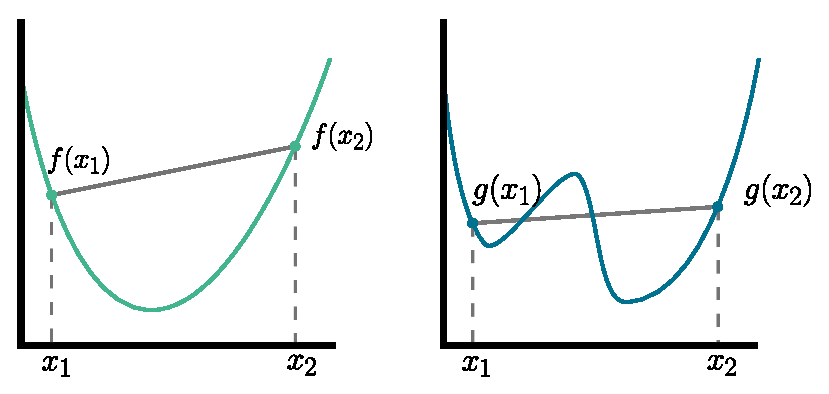
\includegraphics[width=\textwidth]{figures/chapter3/convex.eps}
    \caption{Schematic representation of the idea of complexity. The function $f$ is always below the chord between the points $(x_1, f(x_1))$  and $(x_2, f(x_2))$. For $g$ this is not the case. The figure on the left has a global minimum that can be found by following the gradient of the function $f$. The figure on the right has a local minima that represents a suboptimal set of parameter values.}
    \label{fig:convex}
\end{figure}

\section{The Quantum Perceptron}\label{sec:qperceptron}

In this section we will consider a qubit perceptron at finite temperature that uses a generalization of the classical likelihood function for learning. For this description we use density matrices as a generalized probability framework. Density matrices are used in quantum mechanics to describe statistical ensembles of quantum states (See Appendix \ref{sec:density_matrix}). We will have to formulate the classification problem in terms of these density matrices and come up with a learning rule that preserves Hermiticity, positive semidefiniteness and trace. \newline

\noindent Consider again a classification problem where we have a data set consisting of input vectors $\mathbf{x}\in \mathbb{R}^d$ of length $d$ with corresponding labels $y\in \{1,-1\}$. For this problem the classical negative log-likelihood is given by
\begin{equation}
   \mathcal{L}_{cl} = -\sum_{\mathbf{x}} q(\mathbf{x}) \sum_y q(y|\mathbf{x})\log(p(y|\mathbf{x}; \mathbf{w})).
\label{eq:cl_lh}
\end{equation}
Here, $q(\mathbf{x})$ is the probability of observing $\mathbf{x}$, $q(y|\mathbf{x})$ is the conditional probability of observing label $y$ for data $\mathbf{x}$ and $p(y|\mathbf{x}, \mathbf{w})$ is the proposed model conditional probability distribution of the data.

\subsection{Quantum Data}\label{sec:qm_stats}

To extend the classical likelihood in equation \ref{eq:cl_lh} to the realm of quantum mechanics we will describe the model and the conditional probability $q(y|\mathbf{x})$ in terms of density matrices. 
Consider a classical distribution over two variables, $q(y=1|\mathbf{x})$ and $q(y=-1|\mathbf{x})$. For each $\mathbf{x}$, $q(y|\mathbf{x})$ is a distribution over a single bit $y$, and is fully determined by its conditional expectation value of $y$ given $\mathbf{x}$ written as $ b(\mathbf{x})$,
\begin{align}
    q(y|\mathbf{x}) &= \frac{1}{2}(1+b(\mathbf{x}) y)\nonumber,\\
    \text{with } b(\mathbf{x})&= \frac{1}{M}\left(\sum_{\mathbf{x}^\prime} 
    y^{\prime}\mathds{I}(\mathbf{x}^\prime=\mathbf{x})\right)\label{eq:sample_prob},\\
    \text{and } M &= \sum_{\mathbf{x}^\prime}\mathds{I}(\mathbf{x}^\prime = \mathbf{x})\nonumber.
\end{align}
We count how many times label $y$ occurs for some sample $\mathbf{x}$ and divide it by $M$, the total number of times the sample appears in the data. We define the empirical probability 
\begin{align*}
    q(\mathbf{x}) = \frac{M}{N},
\end{align*}
for $M$ occurrences of $\mathbf{x}$, and $N$ the total number of samples. We now note that the diagonal of a density matrix defines a classical probability distribution, since its entries must be positive and sum to one due to the trace constraint. In other words, we can write the classical distribution $q(y|\mathbf{x})$ as a mixed state density matrix,
\begin{equation*}
    \eta_{cl} = q(y=1|\mathbf{x}) \ket{1}\bra{1} + q(y=-1|\mathbf{x}) \ket{0}\bra{0} = 
    \begin{pmatrix}
    q(y=1|\mathbf{x}) & 0\\
    0 & q(y=-1|\mathbf{x})
    \end{pmatrix}.
\end{equation*}
Instead of representing the data with a statistical ensemble $q(y|\mathbf{x})$, we represent the data with the following wave function:
\begin{equation*}
    \ket{\psi} = \sqrt{q(y=1|\mathbf{x})}\ket{1} + \sqrt{q(y=-1|\mathbf{x})}\ket{0}.
\end{equation*}
The density matrix belonging to this pure state is given by
\begin{equation*}
\eta_\mathbf{x} = \ket{\psi}\bra{\psi}=
    \begin{pmatrix}
    q(y=1|\mathbf{x}) & \sqrt{q(y=1|\mathbf{x})}\sqrt{q(y=-1|\mathbf{x})} \\
    \sqrt{q(y=1|\mathbf{x})}\sqrt{q(y=-1|\mathbf{x})} & q(y=-1|\mathbf{x})
    \end{pmatrix}.
\end{equation*}
Which reduces to a classical probability distribution if $q(y=1|\mathbf{x}) \in \{0,1\}$, so that the matrix becomes diagonal.\newline

\noindent All density matrices can be represented by a vector in the Bloch sphere (see Appendix \ref{sec:qubits}). If we look at the Bloch sphere in figure \ref{fig:classic_bloch}, we see that we can only represent the data distribution along the z-axis, $\mathbf{r}_{cl} = (0,0,q(y=1|\mathbf{x})-q(y=-1|\mathbf{x})) = (0,0,2q(y=1|\mathbf{x})-1)$.
However, the quantum representation of the data makes use of an extra degree of freedom on the Bloch sphere as can be seen in figure \ref{fig:classic_bloch2}. 
\begin{figure}[ht!]
    \centering
    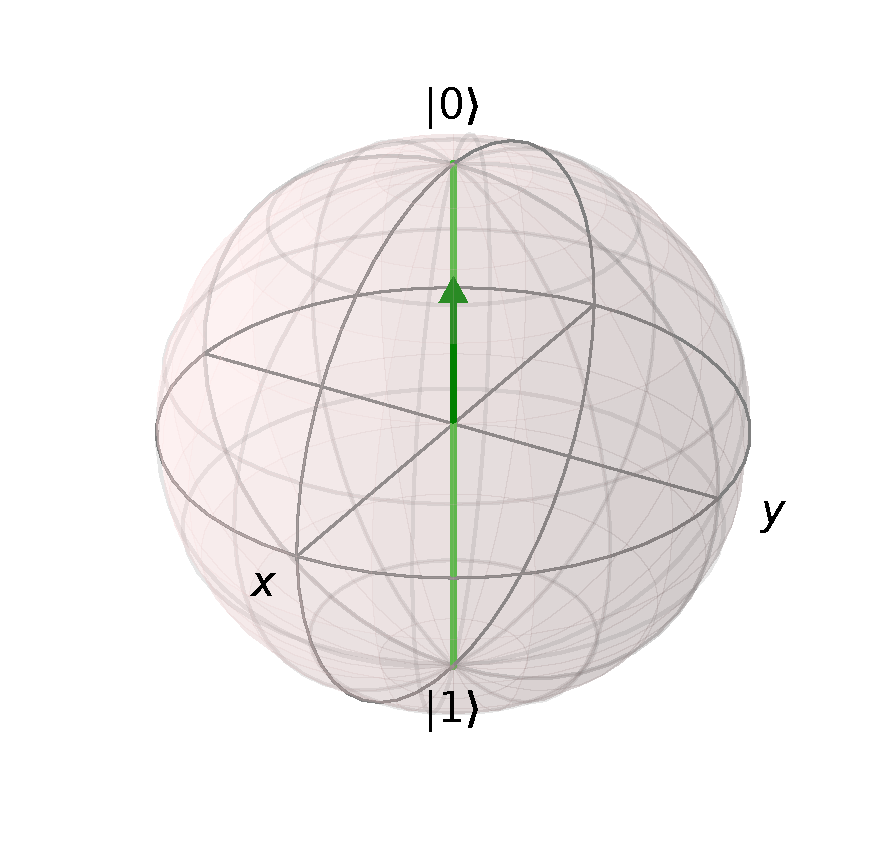
\includegraphics[width=0.6\textwidth]{figures/chapter3/bloch_sphere_2a.pdf}
    \caption{Classical data density matrix. The Bloch vector is confined to z-axis (light green) and has length $|\mathbf{r}|\leq1$. Since the data density matrix is always real, the vector must have $r_y=0$}
    \label{fig:classic_bloch}
\end{figure}

\begin{figure}[htb!]
    \centering
    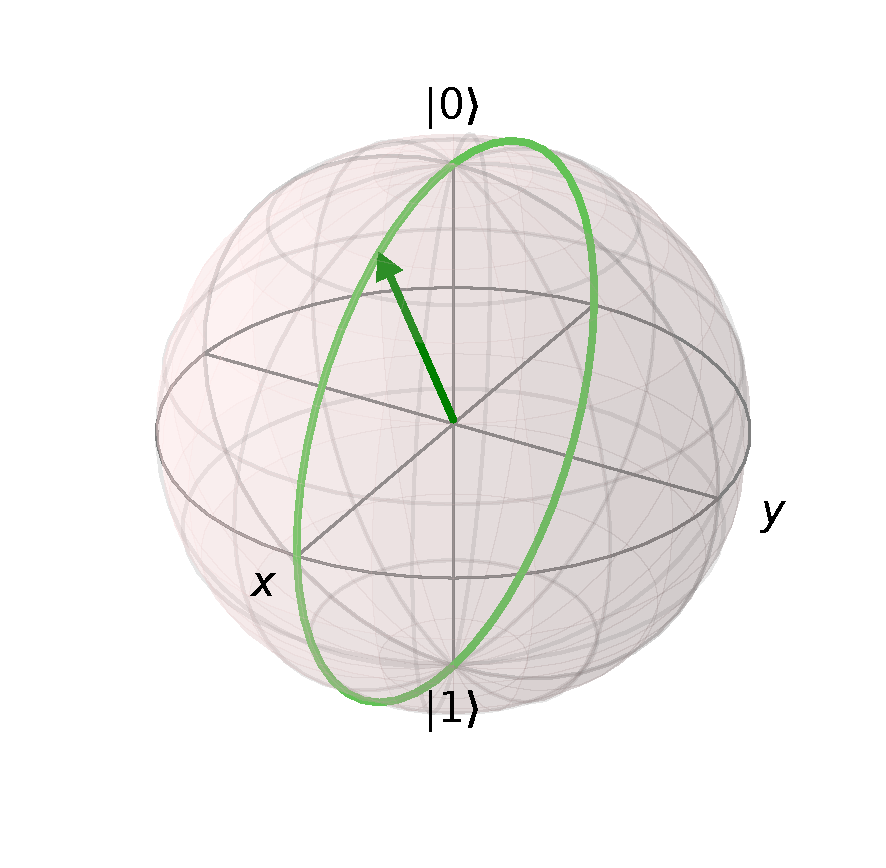
\includegraphics[width=0.6\textwidth]{figures/chapter3/bloch_sphere_2b.pdf}
    \caption{Quantum data density matrix. The Bloch vector is confined to the surface(light green) of the sphere and has length $|\mathbf{r}|=1$.}
    \label{fig:classic_bloch2}
\end{figure}

\noindent We now propose a quantum model parametrized by a density matrix $\rho(\mathbf{x}, \mathbf{w}; y, y^\prime)\equiv \rho_\mathbf{x}$,
\begin{equation*}
    \rho_\mathbf{x} = \frac{1}{Z} e^{-\beta H}\label{eq:density},
\end{equation*}
where $H = \sum_k h^k \sigma^k$, with $h^k \in \mathbb{R}$ and $\sigma^k$ the Pauli matrices with $k = (x,y,z)$ from equation \ref{eq:pauli_mats}. This is a finite temperature description of a qubit, where we will set $\beta=-1$ for now. If $\rho_\mathbf{x}$ is diagonal, this model reduces to the Boltzmann distribution of equation \ref{eq:log_reg}. We can absorb the inverse temperature $-\beta$ in the field $-\beta h^k \to h^k$ by rescaling the weights $\mathbf{w}^k$. Using that 
\begin{equation*}
    e^{a \hat{n}\cdot \bm{\sigma}} = \cosh{a} + \sinh{a}\sum_k \sigma^k,
\end{equation*}
and writing $\sum_k h^k \sigma^k = h \sum_k \frac{h^k}{h} \sigma^k = $ with $h = \sqrt{\sum_k(h^k)^2}$ we find
\begin{equation*}
    \rho_\mathbf{x} = \frac{1}{Z}\left( \cosh{h} + \sinh{h}\sum_k \frac{h^k \sigma^k}{h}\right).
\end{equation*}
Solving $\Tr{\rho}=1$ gives $Z = 2 \cosh{h}$. If we plug this in we get
\begin{align}
    \rho_\mathbf{x} & = \frac{1}{2} \mathbb{1} + \frac{1}{2} \tanh{h}\sum_k \frac{h^k \sigma^k}{h}\nonumber \\
    &= \frac{1}{2} \left(\mathbb{1} + \sum_k m^k \sigma^k\right),
    \label{eq:density_matrix_basis}
\end{align}
where $\mathbb{1}$ is a $2\times2$ identity matrix and $m^k = \tanh{h}\frac{h^k}{h}$. Equation \ref{eq:density_matrix_basis} gives us the general description of qubit that we established in section \ref{sec:qubits}. This definition spans the full space of $2\times2$ Hermitian matrices, for all $h^k\in \mathbb{R}$. From the definition of $m^k$ it is clear that $m^k\in(-1,1)$. This means that $\rho_\mathbf{x}$ is positive semidefinite because the eigenvalues of $\rho_\mathbf{x}$ are $\lambda_{\pm} = \frac{1}{2}(1 \pm \sqrt{ \sum_k (m^k)^2}) \geq 0$. From the eigenvalues we also see that $\rho_\mathbf{x}$ describes a mixed state, since it is only rank one if $\sum_k (m^k)^2 = 1$. We parametrize the field $h^k\to h^k(\mathbf{x})$ by setting $h^k(\mathbf{x}) = \mathbf{w}^k\cdot \mathbf{x}$ with $\mathbf{w}^k \in \mathbb{R}^d$, so that the qubit state is dependent on classical input data. To clean up the notation we omit the argument of $h^k$. \newline

\noindent To summarize, the model density matrix can learn a mixed state density matrix that corresponds best to the quantum representation of the data. Since it is mixed, we can move in the interior of the circle of the Bloch sphere, as can be seen in figure \ref{fig:classic_bloch3}. The classical perceptron tries to minimize the likelihood with respect to a classical distribution, that is located on a single axis with interval $[0,1]$. The quantum description of the data is more expressive and contains additional information about the underlying distribution. We will now construct a cost function that minimizes the distance between density matrices, analogous to the cross entropy. This model will make use of the additional degree of freedom on the Bloch sphere to provide a more expressive model.
\begin{figure}[htb!]
    \centering
    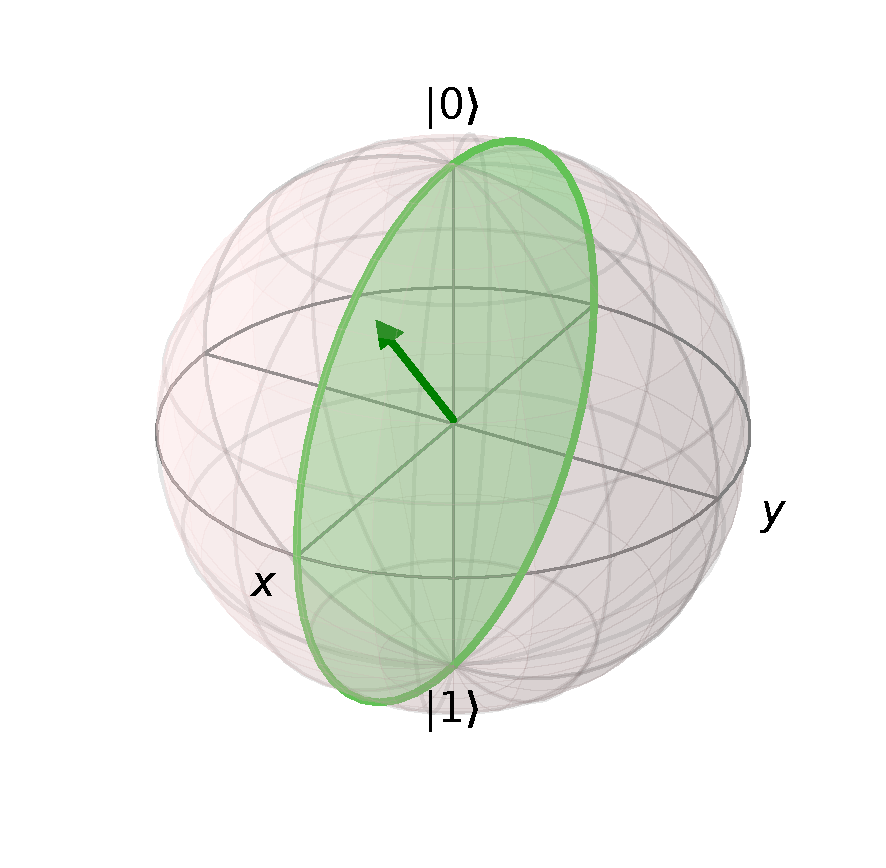
\includegraphics[width=0.6\textwidth]{figures/chapter3/bloch_sphere_2c.pdf}
    \caption{Quantum perceptron model distribution. The Bloch vector can now also lie in the interior of the surface (light green) of the sphere and has length $|\mathbf{r}|\leq1$. We will show later on that the $r_y$ component will always go to zero, so the vector is confined to the $xz$-plane}
    \label{fig:classic_bloch3}
\end{figure}

\subsection{Quantum Likelihood}

We define the quantum conditional likelihood as a cross entropy between a conditional data density matrix $\eta_\mathbf{x}$ and a model conditional density matrix $\rho_\mathbf{x}$, analogous to equation \ref{eq:cl_lh},
\begin{equation}
    \mathcal{L}_{q} = -\sum_{\mathbf{x}} q(\mathbf{x}) \Tr{\eta_\mathbf{x}\log(\rho_\mathbf{x})}.
    \label{eq:q_like}
\end{equation}
This is the quantum mechanical equivalent of the classical log-likelihood which minimizes the ``distance" between the density matrix representations of the data and the model. Next, we rewrite this with the parametrized $\rho_\mathbf{x}$,
\begin{align*}
    & \mathcal{L}_{q} = -\sum_{\mathbf{x}} q(\mathbf{x}) \Tr{\eta_\mathbf{x}\log(\rho_\mathbf{x})} \\
    &= -\sum_{\mathbf{x}} q(\mathbf{x}) \sum_{y,y^\prime} \bra{y\prime}\sqrt{q(y|\mathbf{x})} \sqrt{q(y^{\prime}|\mathbf{x})}\log(\rho_\mathbf{x})\ket{y},
\end{align*}
with $\{\ket{y}\}$ a set of orthonormal vectors in the $\sigma^z$ basis. Then,
\begin{align}
    &=-\sum_{\mathbf{x}} q(\mathbf{x}) \sum_{y,y^\prime} \sqrt{q(y|\mathbf{x})} \sqrt{q(y^{\prime}|\mathbf{x})}\bra{y\prime}\left(\sum_k h^k \sigma^k - \log(2\cosh{h})\right)\ket{y}
    \label{eq:intermed_step}.
\end{align}
Calculating the statistics for the Pauli matrices gives
\begin{align*}
    \sum_{y,y^\prime}\bra{y^\prime} \sum_k h^k \sigma^k \ket{y} &= \sum_{y, y^\prime}\sum_k \bra{y^\prime}h^k \sigma^k \ket{y},
\end{align*}
which gives three delta functions that we can plug into equation \ref{eq:intermed_step} together with the definition of $q(y|\mathbf{x})$ from equation \ref{eq:sample_prob}. Then, 
\begin{align*}
    &\sum_{y, y^\prime} \sqrt{q(y|\mathbf{x})} \sqrt{q(y^{\prime}|\mathbf{x})} \left( h^x \delta_{y^\prime,-y} + i y h^y \delta_{y^\prime,-y} + y h^z \delta_{y^\prime,y} \right)\\
    &= \sum_y h^x \frac{1}{2}\sqrt{1 + b(\mathbf{x}) y} \sqrt{1 - b(\mathbf{x}) y} + i y h^y\frac{1}{2} \sqrt{1 + b(\mathbf{x}) y}\sqrt{1 - b(\mathbf{x}) y} + y h^z\frac{1}{2}\sqrt{1 + b(\mathbf{x}) y }  \sqrt{1 + b(\mathbf{x}) y} \\
    &=h^x \sqrt{1 - b(\mathbf{x})^2} + h^z b(\mathbf{x}).
\end{align*}
The $h^x$ term quantifies how often a sample occurs with a flipped output label and is the distinguishing factor from the classical perceptron. The source of this term is the $\sigma^x$ matrix in the likelihood which flips the state $\ket{y}$ and scales $h^x$ with the off-diagonal elements of $\eta_\mathbf{x}$. As a final likelihood we get
\begin{align}
    \mathcal{L}_{q} &= -\sum_{\mathbf{x}} q(\mathbf{x})  \bigg(h^x \sqrt{1 - b(\mathbf{x})^2} + h^z b(\mathbf{x}) - \log(2\cosh{h})\bigg)\label{eq:final_likelihood}.
\end{align}
In order to perform learning we have to find update rules that minimize the function in equation \ref{eq:final_likelihood}. To find the minimum we perform gradient descent to update the parameters $\mathbf{w}^k$. Derive with respect to $\mathbf{w}^k$ to obtain
\begin{align}
    \frac{\partial \mathcal{L}_{q}}{\partial \mathbf{w}^x} &= -\sum_{\mathbf{x}} q(\mathbf{x})  \left(\sqrt{1 - b(\mathbf{x})^2}  - \tanh{h} \frac{h^x}{h}\right)\mathbf{x}\nonumber,\\
    \frac{\partial \mathcal{L}_{q}}{\partial \mathbf{w}^y} &= \sum_{\mathbf{x}} q(\mathbf{x}) \tanh{h} \frac{h^y}{h} \mathbf{x}\nonumber,\\
    \frac{\partial \mathcal{L}_{q}}{\partial \mathbf{w}^z} &= -\sum_{\mathbf{x}} q(\mathbf{x})  \left( b(\mathbf{\mathbf{x}}) - \tanh{h} \frac{h^z}{h} \right)\mathbf{x} \label{eq:grads},
\end{align}
and update the weights at iteration $t$ with
\begin{align}
    \mathbf{w}^k(t+1) =  \mathbf{w}^k(t) - \epsilon \left(\frac{\partial \mathcal{L}}{\partial \mathbf{w}^k(t)}\right).
    \label{eq:grad_desc}
\end{align}
These are the learning rules for the quantum perceptron, with learning parameter $\epsilon$ for each gradient. Since the gradient step of $\mathbf{w}^y$ is proportional to $\mathbf{w}^y$, the fixed point solution is $\mathbf{w}^y\rightarrow\bm{0}$ in the limit of many iterations. In the case that there exists a function $f(\mathbf{x}) = y$ (no noise in the data) for all data points, the statistics $b(\mathbf{x})$ become either $1$ or $-1$, which gives a fixed point solution $\mathbf{w}^x\rightarrow\bm{0}$. The $z$ field then corresponds to the single field of a classical perceptron (see section \ref{sec:cl_percp}) and the quantum perceptron approaches the classical case. However, in the case that there are samples which have both $1$ and $-1$ labels, the weight $\mathbf{w}^x$ becomes finite and the solution of the quantum perceptron will diverge from the classical perceptron. This change in behaviour is reflected in the probability boundaries, which differ from the classical case as we will see in section \ref{sec:probs}.

\subsection{Convexity of the Quantum Log-Likelihood}\label{sec:convexity_qlh}

To prove the convexity of the likelihood function, we only look at the expression $\eta_\mathbf{x} \log (\rho_\mathbf{x})$. It is known that the relative entropy
\begin{equation*}
    S(\rho || \sigma) = \Tr{\rho \log(\rho)} - \Tr{\rho \log(\sigma)},
\end{equation*}
is jointly convex \cite{Carlen2009}. This means that for any $\rho_0, \rho_1, \sigma_0, \sigma_1 \geq 0$
\begin{equation*}
    S((1-t)\rho_0 + t \rho_1 || (1-t)\sigma_0 + t \sigma_1) \leq (1-t) S(\rho_0||\sigma_0) + t S(\rho_1||\sigma_1),
\end{equation*}
which implies that $S(\rho || \sigma)$ is strictly convex in $\rho$ and that thus $\eta_\mathbf{x} \log (\rho_\mathbf{x})$ is convex in $\rho_\mathbf{x}$. Similar to the classical case, the cost function is convex, so we will find a global minimum with gradient descent.

\section{Predicting Classes}

Once the model is trained, we can construct a state $\rho_\mathbf{x}$ for the qubit based on some input $\mathbf{x}$. From the definition in equation \ref{eq:density_matrix_basis} we get
\begin{equation*}
        \rho_\mathbf{x} = \frac{1}{2}\begin{pmatrix}
           1 + m^z  & m^x - im^y\\
           m^x + im^y      & 1 - m^z          
        \end{pmatrix}.
\end{equation*}
The eigenvectors of the learned density matrix correspond to the physical states of the model qubit system. By decomposing the density matrix into rank one density matrices composed of the eigenvectors $\{\ket{\psi}\}$ we get
\begin{equation}
    \rho = \sum_i p_i \rho_i = \sum_i p_i \ket{\psi_i}\bra{\psi_i} = \sum_i \lambda^2_i \ket{\psi_i}\bra{\psi_i}.
    \label{eq:density_matrix_lambdas}
\end{equation}
where the probabilities $p_i$ correspond to the squares of the respective eigenvalues $\lambda_i$ for each eigenvector $\ket{\psi_i}$ of the density matrix. The learned model thus contains two levels of probabilities:
\begin{enumerate}
    \item $\lambda_i^2$: the classical probability of finding the system in eigenstate $i$
    \item $\ket{\psi_i}$: the quantum probability of finding either a $\ket{0}$ or $\ket{1}$ state.
\end{enumerate}
So how do we obtain a class prediction from this model? As we will see, there are several methods to do this. Each method has different qualitative properties that we will explore in the next sections.

\subsection{Eigenvectors \label{sec:probs}}

To start off, we will determine the eigenvalues and eigenvectors of the model,
\begin{align}
    \lambda_{\pm} = \frac{1}{2}\left(1 \pm \sqrt{\sum_k m^k}\right) = \frac{1}{2}(1 \pm \Tilde{m}).
    \label{eq:eigenvalue}
\end{align}
The orthonormal eigenvectors corresponding to each eigenvalue are
\begin{align}
    \mathbf{v}_+ &= \frac{1}{Z}
    \begin{pmatrix}
        m^z + \Tilde{m}\\
        m^x + im_y\\
    \end{pmatrix} \nonumber ,\\
    \mathbf{v}_- &=  \frac{1}{Z}
    \begin{pmatrix}
        -m^x + im^y\\
        m^z + \Tilde{m}
    \end{pmatrix}.
    \label{eq:eigenvector}
\end{align}
with the normalization factor given by $Z = \sqrt{\mathbf{v}_{\pm} \cdot \mathbf{v}_{\pm}^*}$,
\begin{align*}
    \mathbf{v}_\pm \cdot \mathbf{v}^*_\pm &=  \left((m^z)^2 + \Tilde{m}^2 + 2m^z\Tilde{m} + (m^x)^2 + (m^y)^2 \right) \\
    &= 2\Tilde{m}(\Tilde{m} + m^z),
\end{align*}
which gives the eigenvectors the desired properties $\langle\mathbf{v}_+,\mathbf{v}_-\rangle = \delta_{+-}$. There appear to be singularities for  
\begin{align*}
    m^z &= \Tilde{m} = \sqrt{\sum_k (m^k)^2}\\
    (m^z)^2 &= \sum_k (m^k)^2\\
    (m^x)^2 &= -(m^y)^2
\end{align*}
But for $m^k\in \mathbb{R}$ this is only singular for $m^x=m^y=0$, which is the limiting case for no noise in the data. This gives $\Tilde{m}=1$, so the system become rank one. This could lead to some numerical instability during learning, but no problems have been encountered while obtaining the results in this thesis. The system can only become degenerate in the case that $\Tilde{m}\to0$. This solution is rather unlikely, since this would imply that the fixed point of $\mathbf{w}^z=0$ which is only possible if $b(\mathbf{x})=0$ for all $\mathbf{x}$. In the following sections we will discuss different methods to construct a probability from the eigenvectors.

\subsection{Proposal 1: Rank One Approximation} 

The first proposal looks at the largest eigenvector $\mathbf{v}_+$. If $\Tilde{m}$ is close to one this eigenvector dominates the system. We can project the eigenstate onto the basis states belonging to the classes $y=\{-1,1\}$, which are the given by the state vectors $\ket{0}=\mathbf{e}_0$ and $\ket{1}=\mathbf{e}_1$. By taking the square of these projections we get properly defined class probabilities,
\begin{align}
    p(y=1|\mathbf{x};\mathbf{w}) &= |\mathbf{e}_0 \cdot \mathbf{v}|^2 = |v_1|^2 \label{eq:v1},\\
    p(y=-1|\mathbf{x};\mathbf{w}) &= |\mathbf{e}_1 \cdot \mathbf{v}|^2 = |v_2|^2 \label{eq:v2},
\end{align}
where $\langle \mathbf{v},\mathbf{v}\rangle = 1$ by construction, so $|v_1|^2 + |v_2|^2 = 1$. Taking $m^y\to0$ allows us to write the largest eigenvector from equation \ref{eq:eigenvector} as
\begin{align*}
p(y|\mathbf{x};\mathbf{w}) = 
    \begin{pmatrix}
        v_1^2\\
        v_2^2
    \end{pmatrix}    =
     \frac{1}{2\Tilde{m}(m^z + \Tilde{m})}
    \begin{pmatrix}
        (m^z + \Tilde{m})^2\\
        (m^x)^2
    \end{pmatrix}.
\end{align*}
Using that $(m^x)^2 = \Tilde{m}^2 - (m^z)^2 = (\Tilde{m} + m^z)(\Tilde{m} - m^z)$ we can write
\begin{align*}
   p(y|\mathbf{x};\mathbf{w}) = \frac{1}{2\Tilde{m}(m^z + \Tilde{m})}
    \begin{pmatrix}
        m^z + \Tilde{m}\\
        \Tilde{m} - m^z
    \end{pmatrix}
    =
    \frac{1}{2\Tilde{m}} 
    \begin{pmatrix}
        \Tilde{m} + m^z\\
        \Tilde{m} - m^z
    \end{pmatrix}.
\end{align*}
This probability can be expressed in terms of the output $y$.
\begin{align}
\Aboxed{
    \text{\textbf{Proposal 1:}\hspace{1cm}}  p(y|\mathbf{x};\mathbf{w}) = \frac{1}{2}(1+ y\frac{m^z}{\Tilde{m}})
    }
    \label{eq:prob_ev}
\end{align}
So what kind of model does this give us? We can analytically determine the shape of the boundary separating the two classes, by setting $p(y=1|\mathbf{x};\mathbf{w}) = p(y=-1|\mathbf{x};\mathbf{w})$. 

\begin{align}
    \frac{1}{2}(1 + \frac{m^z}{\Tilde{m}}) &= \frac{1}{2}(1 - \frac{m^z}{\Tilde{m}})\nonumber\\
    \frac{m^z}{\Tilde{m}}& = \frac{h^z}{h} = 0\label{eq:hz_h}.
\end{align}
which is solved for $h^z$=0. The field
\begin{align*}
    h^z = \mathbf{w}\cdot\mathbf{x} =  w_0^z + \sum_i w_i^z x_i^\mu,
\end{align*}
is equal to the equation of a hyperplane, so a linear separation boundary. Let us compare this to the separation boundary for logistic regression. For logistic regression the probability was given by the sigmoid. Setting the probabilities from equation \ref{eq:log_reg} for $y=1$ and $y=-1$ equal gives
\begin{align*}
    \frac{1}{1+e^{-h}} &= \frac{1}{1+e^{h}},
\end{align*}
which is solved for $h=\mathbf{w}\cdot\mathbf{x}=0$. This corresponds to a hyperplane, just as for the quantum perceptron. However, this does not imply that $\mathbf{w}^z = \mathbf{w}$, since both weight vectors belong to the minimum of a different cost function, the quantum log-likelihood and the classical log-likelihood, respectively. Only in the case that there is no noise in the data do the weights coincide. However, both algorithms have a probability boundary that is linear. Significant differences between the two algorithms start appearing when we start looking at the probability curves. These curves describe regions of equal probability through the input space. Algebraically this corresponds to
\begin{equation}
    p(y=1|\mathbf{x};\mathbf{w}) = p(y=-1|\mathbf{x};\mathbf{w})+ \epsilon  \label{eq:p_eps},
\end{equation}
with $\epsilon\in [0,1]$. Using that $p(y=1|\mathbf{x};\mathbf{w}) + p(y=-1|\mathbf{x};\mathbf{w}) = 1$ we get
\begin{align}
    2p(y=1|\mathbf{x};\mathbf{w})& = p(y=-1|\mathbf{x};\mathbf{w}) + p(y=1|\mathbf{x};\mathbf{w})\epsilon \nonumber\\
    p(y=1|\mathbf{x};\mathbf{w}) &= \frac{1}{2}(1 + \epsilon)\label{eq:curve}.
\end{align}
Solving this equation means that we find the boundary separating the space into two parts. One part of the space gets assigned a probability $p(y=1|\mathbf{x};\mathbf{w})>\frac{1}{2}(1 + \epsilon)$ and $p(y=1|\mathbf{x};\mathbf{w})<\frac{1}{2}(1 + \epsilon)$. Combining equations \ref{eq:prob_ev} and \ref{eq:curve} in the limit that $h^y \to 0$ gives
\begin{align*}
    \frac{1}{2}\left(1+\frac{h^z}{\sqrt{(h^x)^2+(h^z)^2}}\right) &= \frac{1}{2}(1 + \epsilon)\\
    \frac{h^z}{\sqrt{(h^x)^2+(h^z)^2}} &= \epsilon\\
    (h^z)^2 &= ((h^x)^2+(h^z)^2) \epsilon^2\\
    (h^z)^2(1-\epsilon^2) &= (h^x)^2 \epsilon^2.
\end{align*}
We need to keep careful track of the minus signs. In the first line, $h^x$ always gives a positive contribution, so we take take the absolute value. But $h^z$ does have a sign, so its sign not impacted by squaring and taking the roots. This gives
\begin{align*}
    h^z &=  \pm \frac{ \epsilon^2}{\sqrt{1- \epsilon^2}} \abs{h^x} \\
    h^z &= \pm\delta \abs{h^x}.
\end{align*}
This equation defines a hyperplane,
\begin{equation*}
    \vecwk{z}\cdot \mathbf{x} \mp \delta\abs{\vecwk{x} \cdot\mathbf{x}}= 0.
\end{equation*}
For $\delta\neq0$ we also require that
\begin{align*}
    \vecwk{x}\cdot \mathbf{x} + w_0^x &= 0\\
    \vecwk{z}\cdot \mathbf{x} + w_0^z &= 0.
\end{align*}
Both these equations do not depend on $\delta$, so all $\delta$-hypersurfaces intersect in the same subspace. Assuming that $\vecwk{x}$ and $\vecwk{z}$ are linearly independent, we can solve for 2 of the $n$ variables in $\mathbf{x}$. This means that the hyperplane intersect in a linear subspace spanned by the $n-2$ free variables of the system of equations. For $n=2$ this means that they intersect in a single point, for $n=3$ a line, $n=4$ a plane and $n=m$ in a $m$-dimensional hypersurface. We can plot these curves for a simple two-dimensional example with bias. See figure \ref{fig:int_qm_exact_mirror} for an example of the curves of the quantum perceptron.
\begin{figure}[htb!]
    \centering
    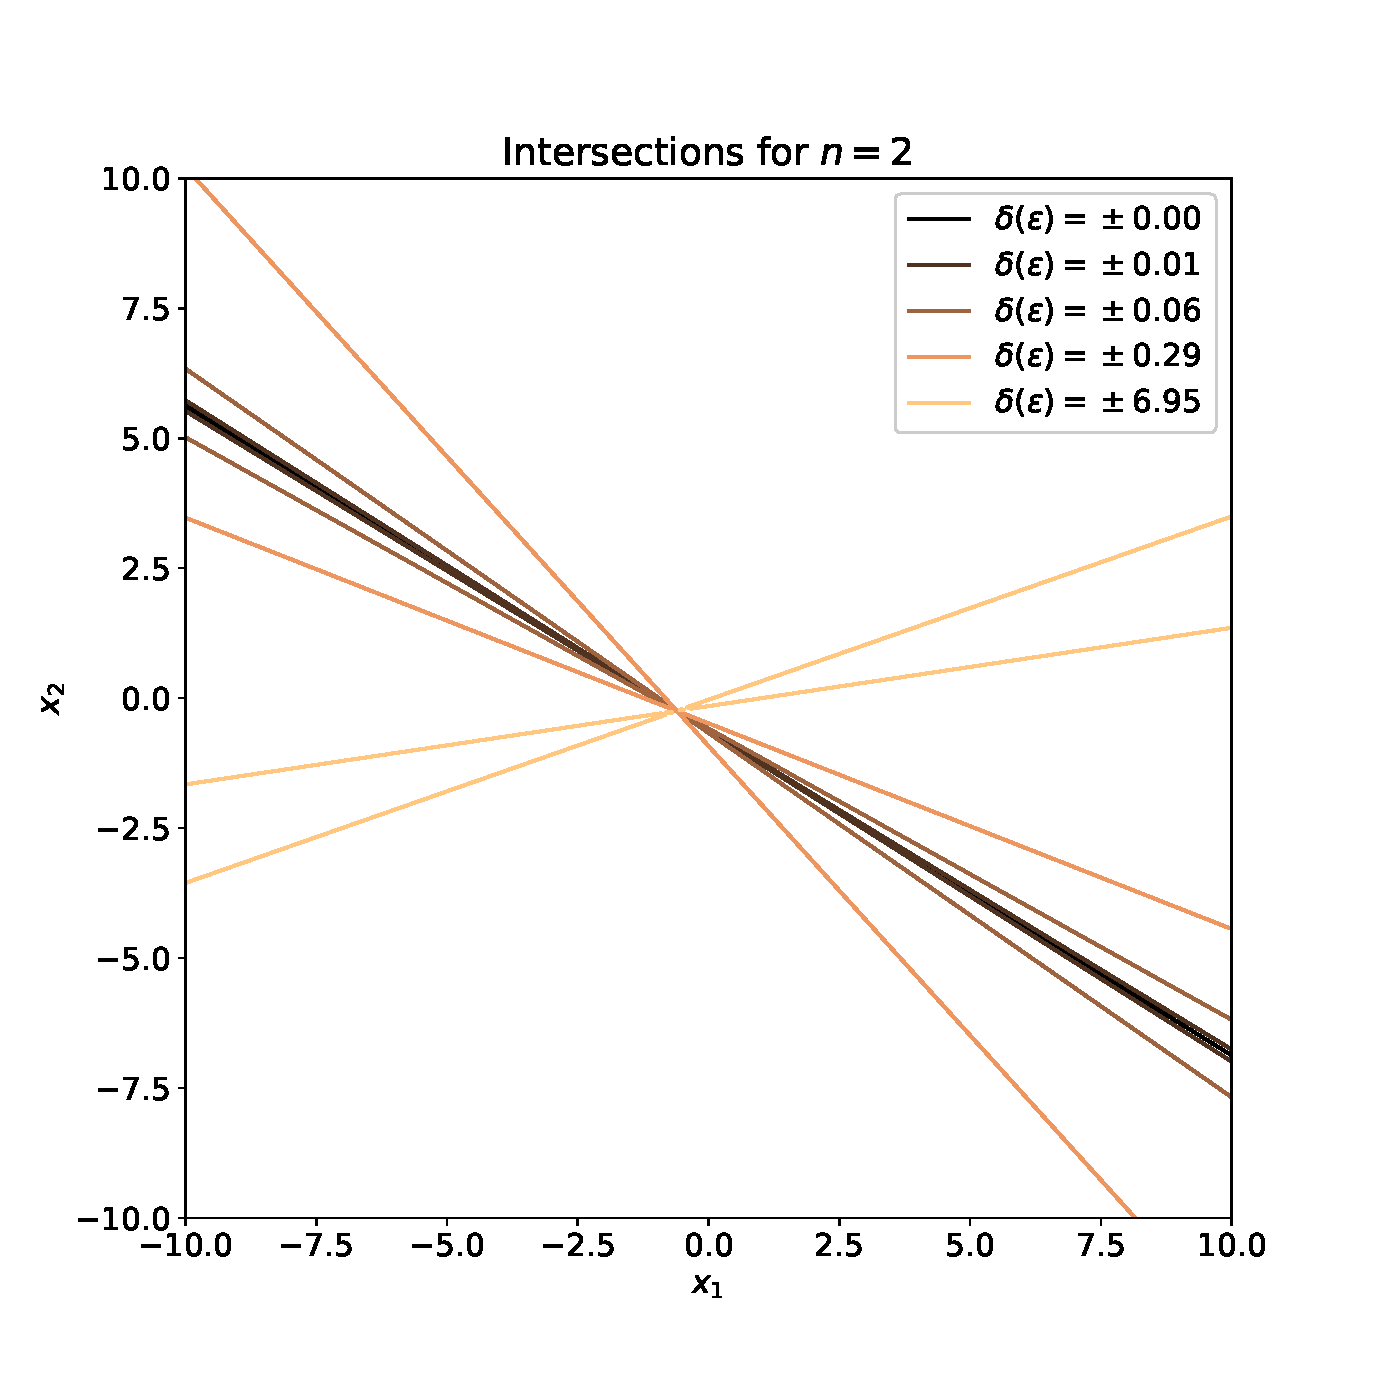
\includegraphics[width = 0.9\textwidth]{figures/chapter3/intersections_qm_exact_mirror.eps}
    \caption{Separation boundaries for the quantum perceptron based on the rank one approximation. The model is given by $\vecwk{x} = (-0.24, 1)$, $w^x_0 = 0.1$ and  $\vecwk{z} = (0.5, 0.8)$, $w^z_0 = 0.5$. Since $\vecwk{x}$ is non-zero we have a noisy problem. Adding the negative $\delta$ contribution provides us with the symmetrical boundaries image. The region in the top right half enclosed by the yellow lines is the region where $p(y=1|\mathbf{x};\mathbf{w})\approx 1$, per equation \ref{eq:curve}. Conversely, for the yellow lines in the bottom left half we have $p(y=-1|\mathbf{x};\mathbf{w})\approx 1$ }
    \label{fig:int_qm_exact_mirror}
\end{figure}
We can also find the boundary given by logistic regression, for small $h$ we approximate $S(h) \approx h$ to get
\begin{align*}
    h &= - h + \epsilon\\
    2h - \epsilon &=  2 \mathbf{w}\cdot\mathbf{x} - \epsilon = 0,
\end{align*}
which is a plane equation with the origin shifted along in the direction $\epsilon \sum_i \mathbf{e}_i$, so planes parallel to the original separation boundary. Of course the approximation $S(h) \approx h$ completely falls flat for $h>2$, since we do not capture the asymptotic behaviour. Without the approximation this becomes
\begin{align*}
    \frac{1}{1+e^{-h}} - \frac{1}{1+e^{h}} &= \epsilon,
\end{align*}
which does not give a nice plane equation, but can be plotted nonetheless. As expected we get linear separation boundaries parallel to the boundary of equal probability. See figure \ref{fig:int_cl_exact_mirror}. The difference between the two models is striking: the classical perceptron can only assign probability boundaries parallel to the separation boundary where the quantum perceptron can assign different titled boundaries to separate areas of probability. In the case of $m^x=0$, we get 
\begin{equation*}
    p(y|\mathbf{x};\mathbf{w}) = \frac{1}{2}\left(1+ y \text{sgn}(x)\right),
\end{equation*}
so a hard step function.
\begin{figure}[ht!]
    \centering
    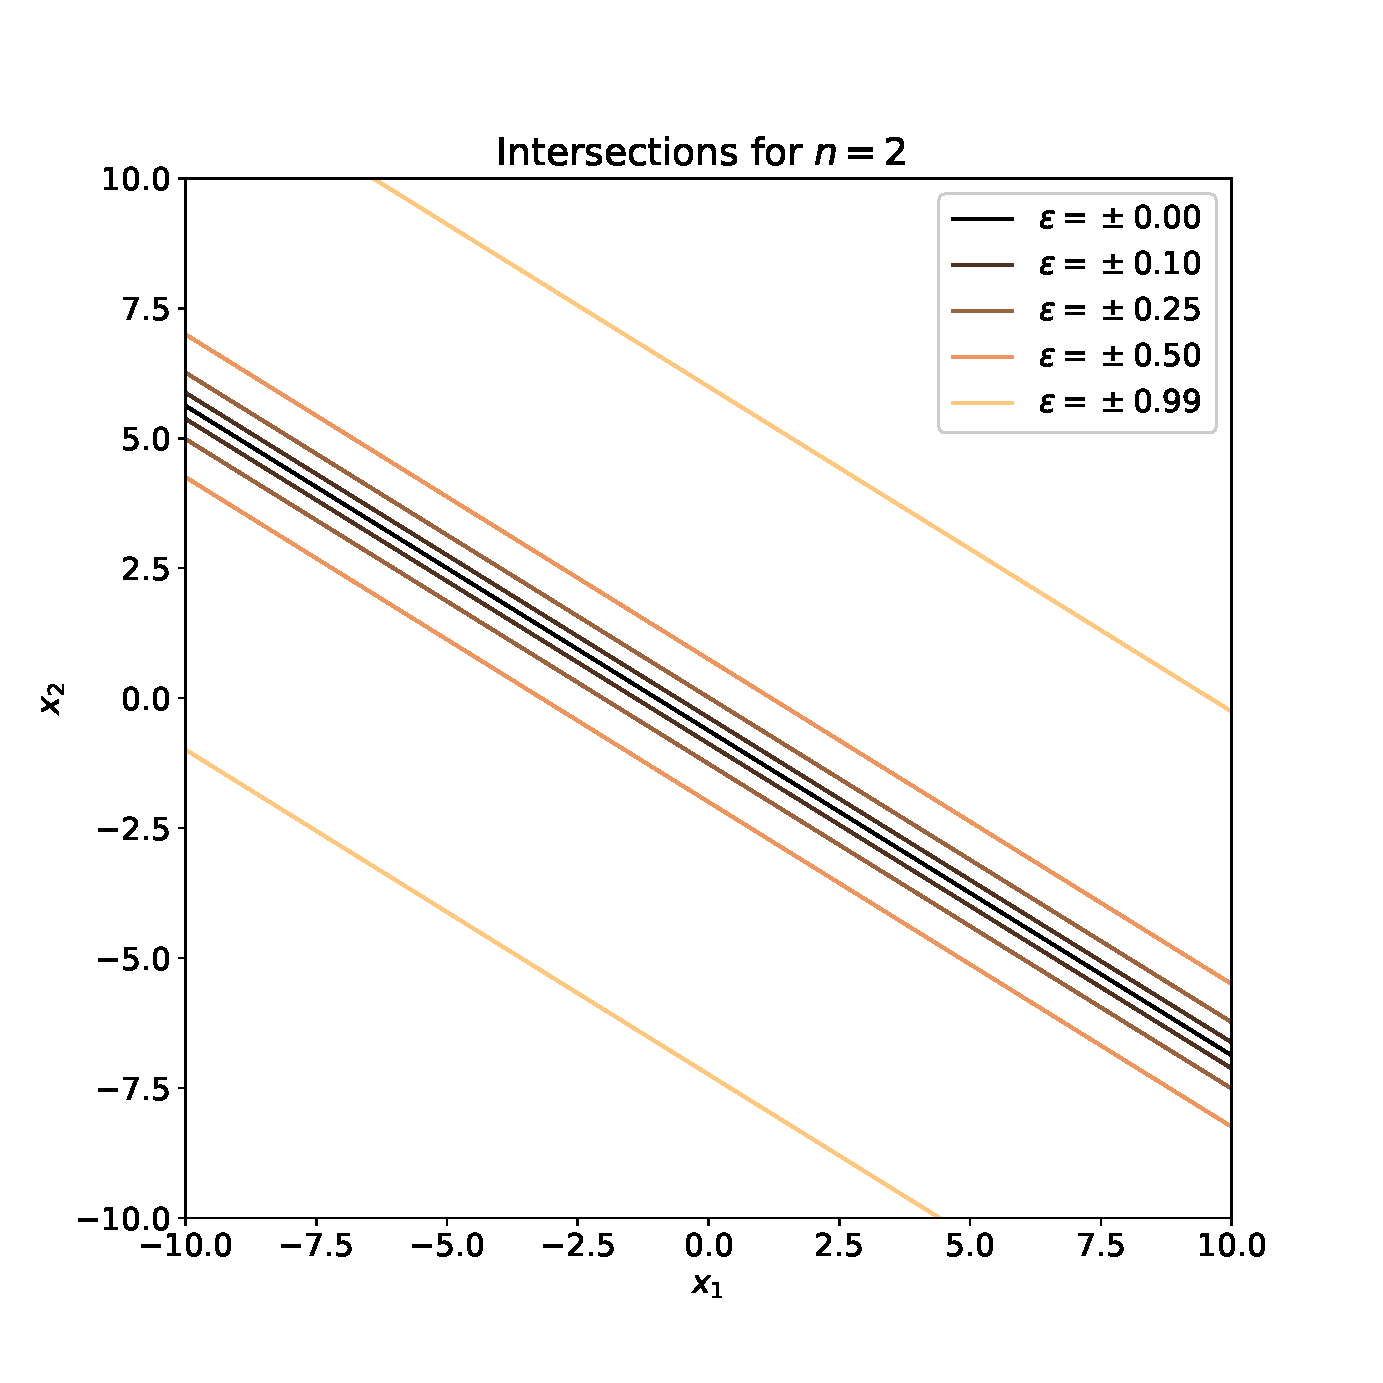
\includegraphics[width = 0.9\textwidth]{figures/chapter3/intersections_cl_exact_mirror.eps}
    \caption{Separation boundaries for logistic regression. For logistic regression we take the $\mathbf{w}^z$ weights of the quantum perceptron, since in the limit of no noise these weights will be equal. The distance between the $\epsilon$-curves is determined by the sigmoid. The closer $\epsilon$ gets to 1, the larger the distance between the lines, which is clear from the shape of the sigmoid and its asymptotic behaviour, as we saw earlier in figure \ref{fig:sigmoid}.}
    \label{fig:int_cl_exact_mirror}
\end{figure}


\subsection{Proposal 2: Quantum Statistics as Boundary \label{sec:mz}}

A more physically-inspired idea is to measure observables that translate naturally to class probabilities. For this system the easiest observables that we can measure are $\expval{\sigma^k}$,
\begin{align*}
   \langle\sigma^k\rangle = \Tr{\sigma^k\rho_\mathbf{x}}.
\end{align*}
With the above definition of $\rho_\mathbf{x}$ we then have 
\begin{align*}
    \Tr{\sigma^k \frac{1}{2}(1 + \sum_{k^\prime} m^{k^\prime} \sigma^{k^\prime})} &= \frac{1}{2}\Tr{\sigma^k + \sum_{k^\prime} m^{k^\prime} \sigma^z\sigma^{k^\prime})}= \frac{1}{2}\bigg(\underbrace{\Tr{\sigma^z}}_{=0} + \sum_{k^\prime} m^{k^\prime} \underbrace{\Tr{\sigma^z\sigma^{k^\prime})}}_{2\delta_{k{k^\prime}}}\bigg) = m^k.
\end{align*}
In other words, we can determine the values of $m^z$ by measuring the spin of the qubit in the $z$ direction. These statistics can then be used to construct a probability of finding the class $p(y)=\frac{1}{2}(1 + y m^z)$. Note that these probabilities are equal to the probabilities of the classical logistic regression in the limit that $m^x$, $m^y$ = 0,
\begin{align*}
    \frac{1}{2}\left(1 + y m^z\right) &=  \frac{1}{2}\left(1 + y \tanh{h}\frac{h^z}{h}\right) = \frac{1}{2}\left(1 + \tanh{y h^z}\right)\\
    & = \frac{1}{2}\left(1 + \frac{e^{yh^z} - e^{-yh^z}}{e^{yh^z} + e^{-yh^z}}\right) = \frac{1}{2}\left(\frac{ e^{yh^z} + e^{-yh^z} + e^{yh^z} - e^{-yh^z}}{e^{yh^z} + e^{-yh^z}}\right) = \frac{ e^{yh^z}}{e^{yh^z} + e^{-yh^z}}\\
    &= \frac{1}{1+e^{-2yh^z}} = S(2yh^z),
\end{align*}
which serves as a motivation for using this description: In the limiting case we get back the logistic regression.
\begin{align*}
    \Aboxed{
    \text{\textbf{Proposal 2:}\hspace{1cm}} p(y|\mathbf{x};\mathbf{w}) = \frac{1}{2}\left(1+ y m^z\right)}
\end{align*}
 We now note something interesting: we can retrieve this proposal with a simple argument by looking at the eigenvectors and eigenvalues from proposal 1. The smallest eigenvector $v_-$ assigns the same probabilities $p(y)$ as $v_+$, but switches the classes,
\begin{align*}
p(y|\mathbf{x};\mathbf{w}) &= 
    \frac{1}{2\Tilde{m}(m^z + \Tilde{m})}
    \begin{pmatrix}
        (m^x)^2\\
        (m^z + \Tilde{m})^2
    \end{pmatrix} = 
    \frac{1}{2\Tilde{m}} 
    \begin{pmatrix}
        \Tilde{m} - m^z\\
        \Tilde{m} + m^z
    \end{pmatrix}\\
     p(y|\mathbf{x};\mathbf{w}) &= \frac{1}{2}(1 - y\frac{m^z}{\Tilde{m}}).
\end{align*}
From equation \ref{eq:density_matrix_lambdas} we can see that the $\lambda_\pm$'s serve as a quantity that tells us how likely one of the eigenstates of the system is. If we take these extra probabilities into account, we get that 
\begin{align*}
    p(y|\mathbf{x};\mathbf{w}) &= \frac{1}{2}(1+ y\frac{m^z}{\Tilde{m}}) \lambda_+ + \frac{1}{2}(1 - y \frac{m^z}{\Tilde{m}})\lambda_- \\
    &= \frac{1}{4}\left((1+ y\frac{m^z}{\Tilde{m}}) (1+\Tilde{m}) + (1 - y \frac{m^z}{\Tilde{m}})) (1-\Tilde{m})\right)\\
    &= \frac{1}{4}\left(1+ \Tilde{m}+y\frac{m^z}{\Tilde{m}}+y m^z + 1 - \Tilde{m} - y \frac{m^z}{\Tilde{m}} + y m^z\right)\\
    &= \frac{1}{2}\left(1+ y m^z\right).
\end{align*}
We can thus conclude that the weighted eigenvector description coincides with measuring $\expval{\sz}$. \newline

\noindent As before, we look the separation boundary and probability boundaries that this model gives. From setting $m^z=0$ it is again clear that the separation boundary is a hyperplane. For the probability boundaries we get
\begin{align*}
    m^z &= \epsilon\\
    \tanh{h}\frac{h^z}{h} &= \epsilon.
\end{align*}
Notice that the hyperbolic tangents and norms do not fall out of the fraction as they did before in equation \ref{eq:hz_h}. This means that the boundaries will not be linear, but curved instead since they are scaled by a nonlinear term. This can be seen in figure \ref{fig:int_tanh}.
\begin{figure}[htb!]
    \centering
    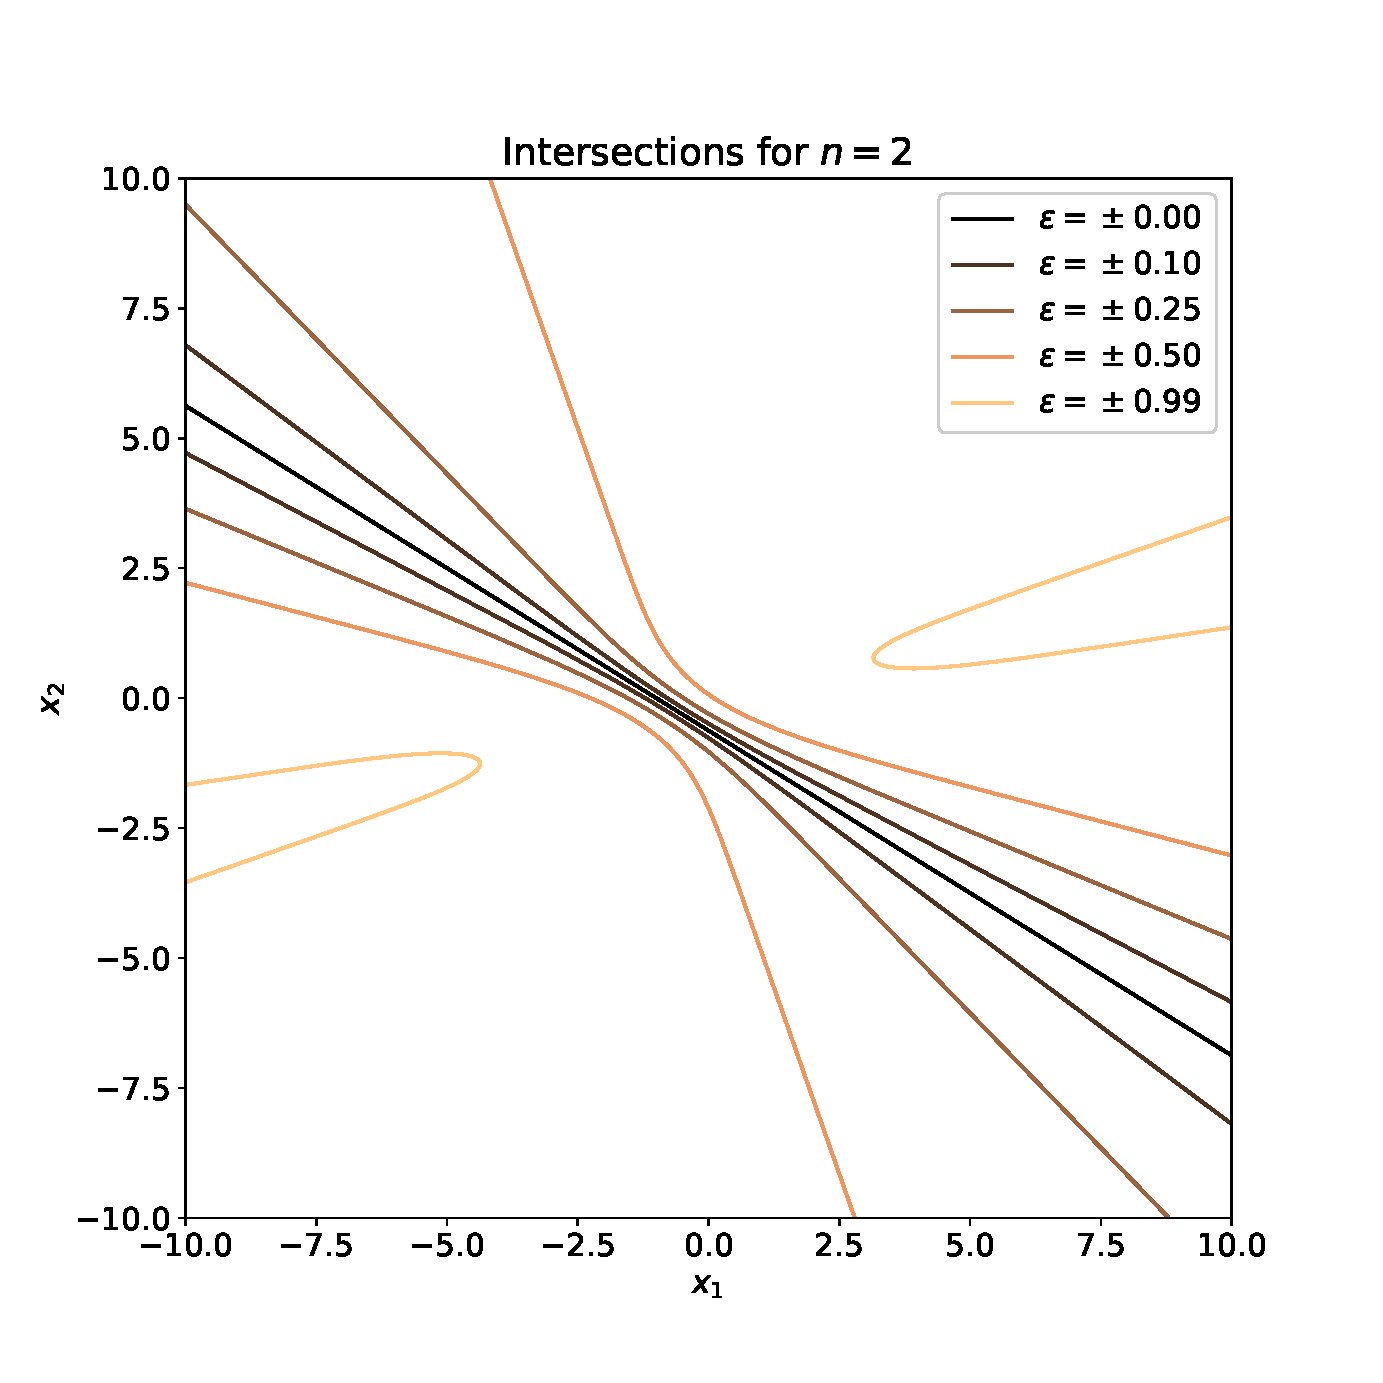
\includegraphics[width=0.9\textwidth]{figures/chapter3/intersections_qm_tanh.eps}
    \caption{Separation boundary for quantum perceptron based on $m^z$ statistics. The previously found boundaries of figure \ref{fig:int_qm_exact_mirror} are now smoothed by the hyperbolic tangent.}
    \label{fig:int_tanh}
\end{figure}
The probability boundaries from the quantum perceptron differ significantly from the logistic regression boundaries in the case of noise. However, the $p(y=1|\mathbf{x};\mathbf{w})=p(y=-1|\mathbf{x};\mathbf{w})$ boundary is still straight. Since the probability curves are only obtained after learning, we cannot really use them to increase classification performance. However, in the case of noise it is possible that the tilted boundaries of the perceptron are better at assigning a more representative probability to a class.

\subsection{Proposal 3: Eigenvector Ellipse}

For completeness we will state this final method to obtain a probability from the eigensystem, even though it is incredibly convoluted. We can describe an ellipse through the equation $\frac{x^2}{a^2} + \frac{y^2}{b^2} = 1$ with $a$, $b$ the semi-major and semi-minor axes, respectively. The eigenvectors of a positive definite matrix span such an ellipse, through the quadratic form
\begin{align*}
    \mathbf{x}^T A \mathbf{x} &= \mathbf{x}^T QDQ^{-1} \mathbf{x} =\mathbf{x}^T \left( 
    (\mathbf{v}_+, \mathbf{v}_-)
    \begin{pmatrix}
    \lambda_+ & 0\\
    0 & \lambda_-
    \end{pmatrix}
    \begin{pmatrix}
    \mathbf{v}_+\\
    \mathbf{v}_-
    \end{pmatrix}
    \right)\mathbf{x}=1,
\end{align*}
with $Q$ the matrix corresponding to the basis transformation to the eigensystem and $Q^{-1} = Q^T$, because the eigenvectors are orthonormal. We see that this description corresponds to an eigenvector rotated to the coordinate system $\mathbf{x}^\prime = \mathbf{x}^T Q$. For the ellipse we have $a = \frac{1}{\sqrt{\lambda_+}}$ and $b = \frac{1}{\sqrt{\lambda_-}}$. Such an ellipse has an area given by $A= ab\pi$, as was already proved by Archimedes in 250 B.C. \cite{Archimedes2009}.\newline

\noindent We now want to consider what area of the ellipse is located in a single quadrant of the output space. This could function as a measure of uncertainty, since the smallest eigenvector can be seen to point in the direction of mislabeled sample in the data density matrix space. If this vector is large, then the area of the eclipse increases proportional to the uncertainty in this direction. The quadrants are given by the lines $y=\pm x$, since this determines the threshold probability when looking at the largest eigenvector. \newline

\noindent We have to determine the intersection of the ellipse with these quadrants and find the corresponding area. Examples of the eigenvector ellipses in the output space are given in figure \ref{fig:ellipse_1} and \ref{fig:ellipse_2}.

\clearpage

\begin{figure}[htb!]
    \centering
    \makebox[\textwidth][c]{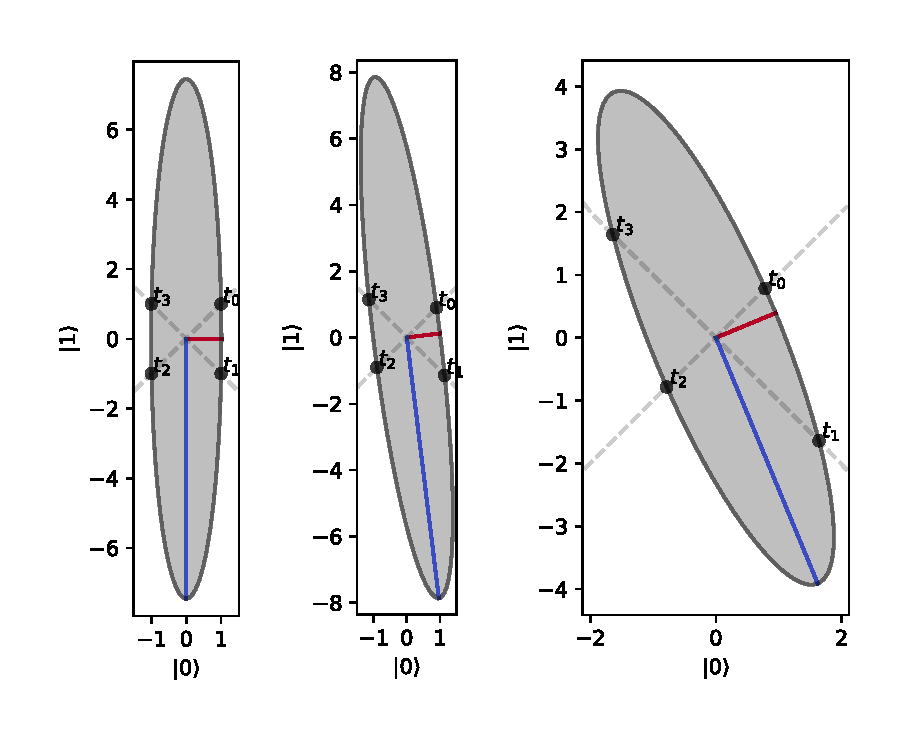
\includegraphics[clip,width=1.\linewidth]{figures/chapter3/combined_ellipses.pdf}}

    \caption{Ellipses spanned by the eigenvectors. The red and blue vectors are the vectors $\mathbf{v_+}$ and $\mathbf{v}_-$ respectively and the $x$-axis and $y$-axis correspond to the directions of $\ket{0}, \ket{1}$ respectively. The vectors are scaled with their corresponding eigenvalues $\lambda_\pm$. The gray dotted lines indicate the quadrants $y=\pm x$ where the intersections are indicated with the dots. The smallest eigenvector increases in length as the amount of uncertainty about the state changes. The ratio of the areas that lie between the lines $y=x\pm$ and the ellipse gives a class label that takes uncertainty into account, since this ratio is affected by the width and rotation of the ellipse. In the left panel we see the eigenvector system for $\mathbf{m} = (10^{-4},\: 0 ,\: 0.96)$. Since $m^x\approx0$, the directions of the eigenvectors align with the directions of the canonical basis $\{\ket{0}, \ket{1}\}$. Even thought there is no uncertainty concerning flipped labels, there is still uncertainty about the correct label, which is indicated by the small area of the ellipse between quadrants $t_0,t_1$ and $t_2, t_3$ ($\ket{0}$-quadrant). The system is close to being pure since $\norm{\mathbf{m}}=0.96<1$. In the middle panel, $\mathbf{m} = (0.44,\: 0,\: 0.87)$. Here, we have $m^x\neq0$ so there are flipped labels which cause a rotation of the ellipse. As a result, more of the mass of the ellipse enters the $\ket{0}$-quadrant. The norm increases to $\norm{\mathbf{m}}=0.97$ so the system becomes purer. Finally, in the left panel we have $\mathbf{m} = (0.63,\: 0 ,\: 0.63)$
    }
    \label{fig:ellipse_1}
\end{figure}

\clearpage

\begin{figure}[htb!]
    \centering
    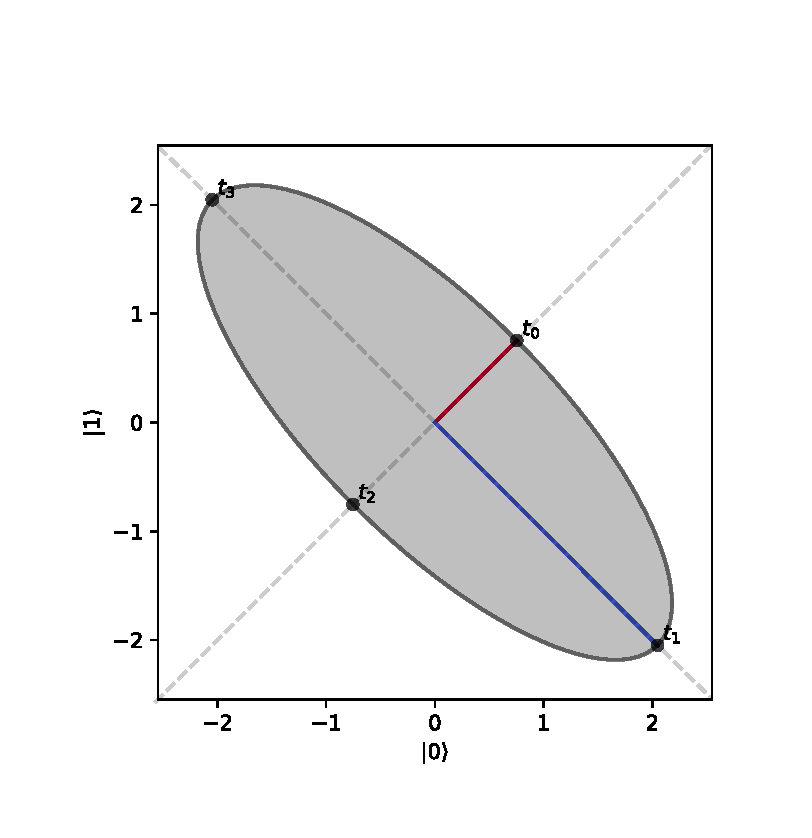
\includegraphics[clip,width=1.\linewidth]{figures/chapter3/combined_ellipses_2.pdf}

    \caption{Ellipses spanned by the eigenvectors. In this final example we have $\mathbf{m} = (0.76,\: 0 ,\: 10^{-4})$. Since $m^z\approx0$ we have maximum uncertainty about the class, which is why the eigenvectors align with the quadrants.}
    \label{fig:ellipse_2}
\end{figure}

\noindent We use the parametric description of the ellipse to calculate the area in a quadrant,
\begin{equation}
    \mathbf{x}_{\text{ellipse}}(t) = \frac{1}{\sqrt{\lambda_+}} \mathbf{v}_+ \cos{t} + \frac{1}{\sqrt{\lambda_-}} \mathbf{v}_- \sin{t}
    \label{eq:parametric_ellipse}
\end{equation}
which when separated in $x$,$y$ components looks as follows
\begin{align*}
    x(t) &= \overbrace{\frac{1}{\sqrt{\lambda_+}} \mathbf{v}_+^x}^{a} \cos{t} + \overbrace{\frac{1}{\sqrt{\lambda_-}} \mathbf{v}_-^x}^{b} \sin{t} = a\cos{t} + b \sin{t},\\
    y(t) &= \overbrace{\frac{1}{\sqrt{\lambda_+}} \mathbf{v}_-^y}^{c} \cos{t} + \overbrace{\frac{1}{\sqrt{\lambda_-}} \mathbf{v}_+^y}^{d} \sin{t} = c\cos{t} + d \sin{t}.
\end{align*}
We solve the equation $y=x$ in Mathematica to get
\begin{align*}
    t_{0,1} = 2 \arctan\frac{b - d \pm \sqrt{a^2 + b^2+ c^2+ d^2 - 2(ac - b d)}}{a - c}
\end{align*}
Solving $y=-x$ gives
\begin{align*}
    t_{2} &= -  \arctan\frac{a+c}{b+d}\\
    t_{3} &= \pi -  \arctan\frac{a+c}{b+d}.
\end{align*}
This gives us the 4 intersections of the ellipse with the lines separating the quadrants. We can now conveniently integrate this ellipse between two intersections at times $t_i$, $t_j$ where $i\neq j$ to find the area in a specific quadrant. For this we use Green's theorem,
\begin{equation*}
    \oint_C (L dx + Mdy) = \iint_D \left(\frac{\partial M}{dx} - \frac{\partial L}{\partial y}\right)dA,
\end{equation*}
which allows us to calculate the area $A$ through the line integral if we choose $\left(\frac{\partial M}{dx} - \frac{\partial L}{\partial y}\right) = 1$, which can be done by setting $L=\frac{1}{2}y$ and $M=-\frac{1}{2}x$,
\begin{equation*}
    \frac{1}{2}\oint_C (y dx - xdy) = \iint_D  dA = A.
\end{equation*}
Clearly we can use this method to calculate the area spanned by the curve between two points. Plugging in the parametric equations $x(t)$ and $y(t)$ gives
\begin{align*}
    A(t_i,t_f) &= \frac{1}{2}\int_{x(t_i)}^{x(t_j)} \left(y(t)dx(t) - x(t)dy(t)\right) = \frac{1}{2}\int_{t_i}^{t_j} \left(y(t)\frac{x(t)}{dt} - x(t)\frac{dy(t)}{dt}\right)dt\\
    &=\frac{1}{2}\int_{t_i}^{t_j}(bc - ad)(\sin^2(t) + \cos^2(t)) = \frac{1}{2}(bc - ad)(t_f - t_j),
\end{align*}
which gives back the Archimedes' result for the total area for the interval $[0, 2 \pi]$:
\begin{equation*}
    2\pi(bc - ad) = \frac{2\pi}{\sqrt{\lambda_+ \lambda_-}} (\mathbf{v}_-^x \mathbf{v}_-^y - \mathbf{v}_+^x \mathbf{v}_+^y) = \frac{\pi}{\sqrt{\lambda_+ \lambda_-}}.
\end{equation*}
where $(\mathbf{v}_-^x \mathbf{v}_-^y - \mathbf{v}_+^x \mathbf{v}_+^y)=1$ since $\mathbf{v}_-$ and $\mathbf{v}_+$ are orthonormal. \newline

\noindent To calculate the amount of probability we determine the ratio of the surfaces in the quadrant of a certain state. 
\begin{align*}
    \Aboxed{
    \text{\textbf{Proposal 3:}\hspace{1cm}} p(y=1|\mathbf{x};\mathbf{w})=\abs{\frac{A(t_0,t_3)}{\frac{1}{2}A_{tot}}} = \frac{(t_3 - t_0)}{(t_3 - t_1)}}
\end{align*}
Similar as before we plot the resulting probability curves in figure \ref{fig:ellipse_boundary}.
\begin{figure}[htb!]
    \centering
    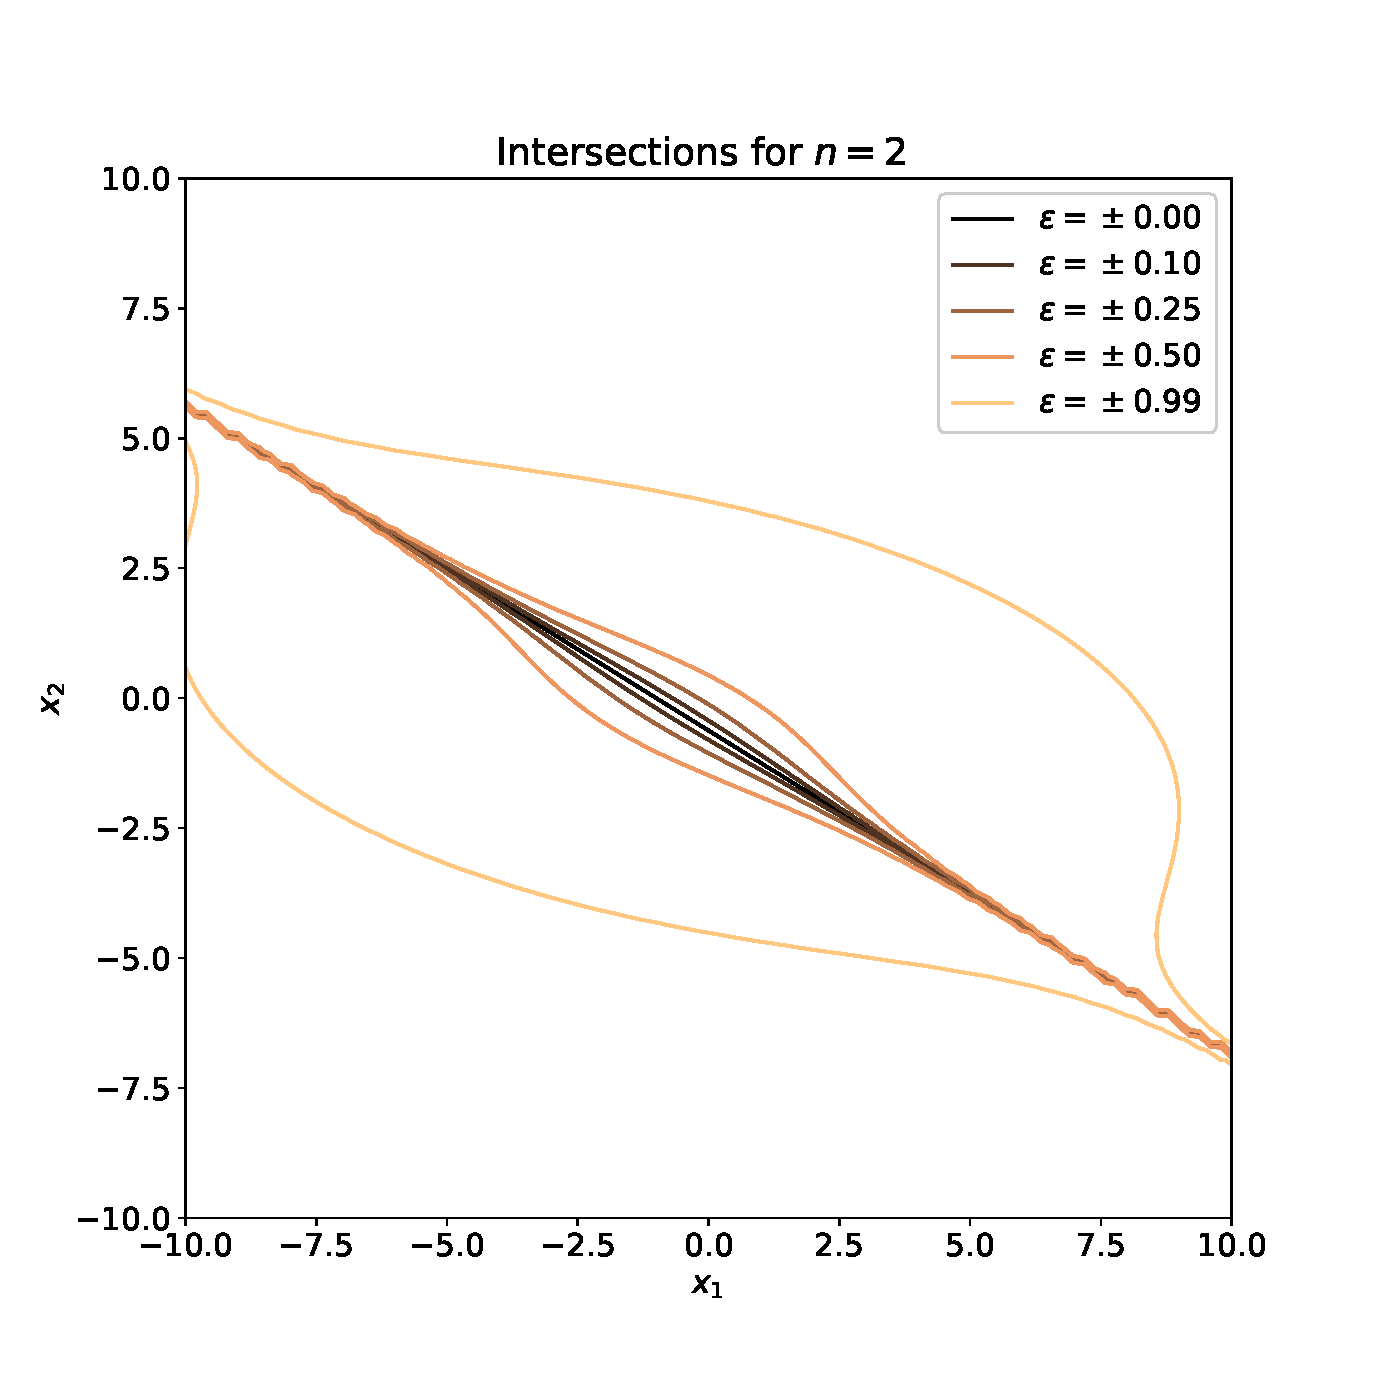
\includegraphics[width = 0.9\textwidth]{figures/chapter3/intersections_ellipse.eps}
    \caption{Separation boundaries for probabilities constructed from the eigenvector ellipse. The line of equal probability is straight as before. It is hard to say something concrete about the shape of the probability boundaries, due to the complexity of the expressions. It seems that the asymptotic behaviour for $\norm{\mathbf{x}}\gg1$ is that the probability boundaries coincide with the separation boundary.}
    \label{fig:ellipse_boundary}
\end{figure}

\subsection{Choosing a class probability}

Looking at these different proposals, using the $m^z$ statistic is the most natural approach that makes the least assumptions. It can directly be connected to the physical world by measuring $\expval{\sigma^z}$. Also, these class probabilities simply correspond to the diagonal values of $\rho_\mathbf{x}$, a fact that will be useful when we extend the model to multiple classes. This approach can be seen as a direct generalization of logistic regression, whereas Proposal 1 is a generalization of the hard sign function. Proposal is more a mathematical exercise, then a well motivated physical measure of probability. For these reasons, we will use Proposal 2 throughout the rest of this thesis as the class probability.

\section{Results}\label{sec:results}

In this section we apply the quantum perceptron to some toy data sets and compare with the classical perceptron with a sigmoid activation function, i.e., logistic regression. For both the classical and quantum perceptron we look at the mean squared error (MSE) to evaluate the performance of both methods,
\begin{equation*}
    \text{MSE} = \frac{1}{N}\sum_{(\mathbf{x},y)} \left(y - p(y|\mathbf{x};\bm{\theta})\right)^2.
\end{equation*}
For each problem we worked with a test set of 20\% of the data. We always reach the global minimum through batch gradient descent because the cost functions are convex for both models. The algorithm is considered converged if the difference of the quantum or classical likelihood $\Delta \mathcal{L} <10^{-7}$. The learning parameter is set to $\epsilon=0.01$ for both algorithms.

\subsection {Simple Two-Dimensional Binary Problem}

In order to demonstrate the difference between the classical and quantum perceptron we consider a two-dimensional binary classification problem. If the problem is linearly separable the classical perceptron converges to a solution where the two classes are perfectly separated. In the case where some samples are mislabeled the quantum perceptron should behave differently, because we account for noise in the learning rule. Consider the data 
\begin{align*}
    \mathbf{x} = \{(1,1), (1,-1), (-1,1), (-1,-1) \},
\end{align*} 
with labels 
\begin{align*}
    y = \{-1,1,-1,-1\}.
\end{align*}  
This problem is trivial since it is linearly separable and all algorithms converge to the same solution ($\mathbf{w}^{x,y}=0$ and $\mathbf{w}_z \approx \mathbf{w}_{cl}$). However, if we flip some of the output labels to simulate mislabeled samples or errors in the data, we suspect that the quantum perceptron will perform better. We make $40$ copies of the $4$  data points in the binary feature space and for $\mathbf{x}\in \{(1,-1),(-1,-1)\}$ we flip $30\%$ of the outputs from $-1$ to $1$. The probability boundaries of the perceptrons differ significantly, as can be seen in figure \ref{fig:boundaries_qm}, which leads to a better assignment of probability the correct states. 

\subsection{Binary Teacher-Student Problem}

A more complex, higher dimensional problem is the Teacher-Student problem where we take a random weight vector $\mathbf{w}_{teacher} \sim \mathcal{N}(0,1)$ and determine labels $y = \text{sgn}(\mathbf{x} \cdot \mathbf{w}_{teacher})$. The input data $\mathbf{x}\in \mathbb{R}^d$ consists of 600 random binary vectors of length $d=8$, where $\mathbf{x}\in\{-1, 1\}^d$. We then create 5 duplicates of each input vector to ensure that there are multiple copies of each sample and attempt to learn 100 different problems where in each run we flip some percentage of the labels. This asserts whether the algorithms can still find the original separation of the data even if noise is introduced. The performance of the quantum perceptron and classical perceptron is compared in figure \ref{fig:lh_diff_mz}.


\begin{figure}[htb!]
    \makebox[\textwidth][c]{
        \subfloat[]{%
            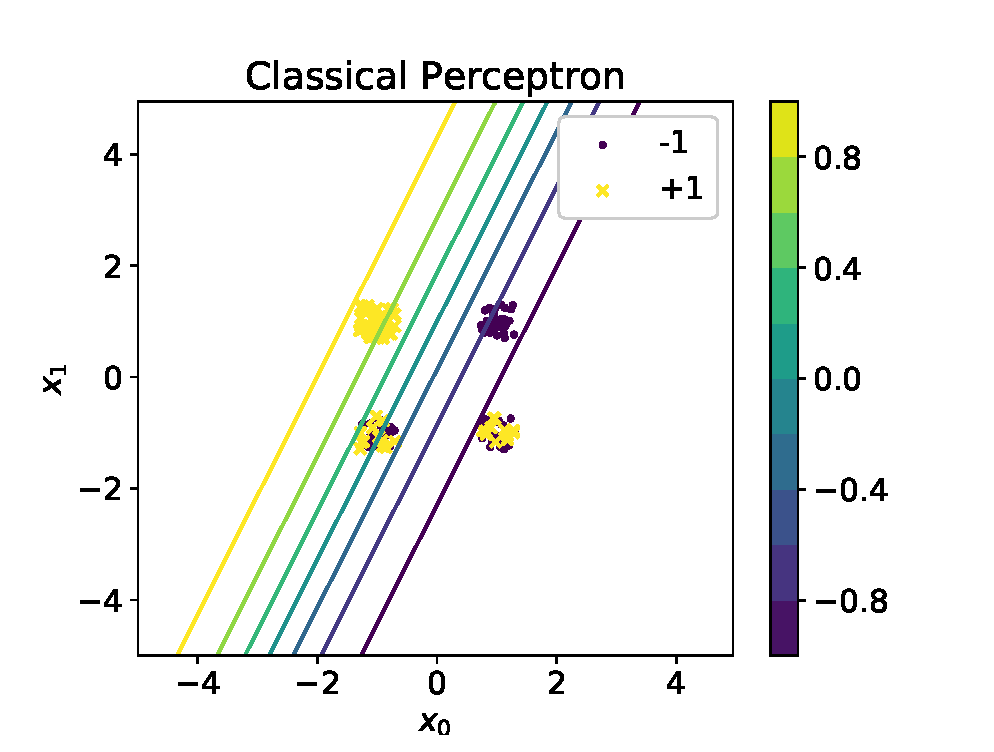
\includegraphics[clip,width=0.7\columnwidth]{figures/chapter3/logistic.eps}
        }
        \subfloat[]{%
            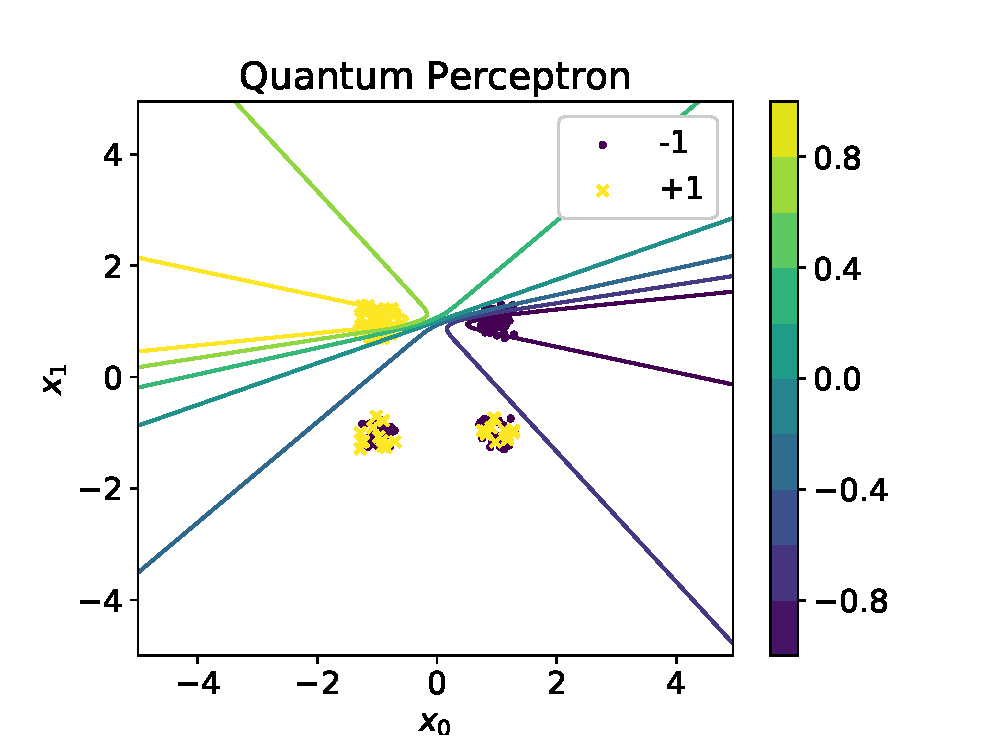
\includegraphics[clip,width=0.7\columnwidth]{figures/chapter3/qperceptron.eps}
        }
    }
    \caption{Separation boundaries in the input space for a two-dimensional problem with $\mathbf{x}=(x_0, x_1)$. The contour lines indicate the expectation value $\mathbb{E}[y|\mathbf{x};\mathbf{w}]_p\in(-1,1)$. The $0.0$-line indicates the separation boundary where $p(y=1|\mathbf{x};\mathbf{w}) = p(y=-1|\mathbf{x};\mathbf{w})=\frac{1}{2}$. Jitter is added to the plot to clarify which samples are noisy. \textbf{(a)} The classical perceptron assigns linear boundaries through the input space, where the distance between the boundaries is scaled with the sigmoid. \textbf{(b)} The quantum perceptron assigns curved boundaries through the input space. Samples with mislabelings get assigned a lower expectation value which results in a lower MSE of $\text{MSE}(quantum) \approx 0.106$ for the quantum perceptron versus $\text{MSE}(classical) \approx 0.154$ for the classical perceptron. Note that if we threshold the quantum perceptron boundary at $p(y=1|\mathbf{x}; \bm{\theta}) = 0.5$, we get a linear boundary that would assign similar classes as in figure (a), even though the boundary is tilted with respect to the classical boundary. However, the quantum perceptron assigns high probabilities to classes about which it is certain ($\mathbf{x}\in \{(-1,1),(1,1)\}$) and lower probabilities to classes about which it is uncertain ($\mathbf{x}\in \{(-1,-1),(1,-1)\}$). The classical perceptron does this significantly worse, which is reflected in the difference in MSE.}
    \label{fig:boundaries_qm}
\end{figure}
\clearpage
\begin{figure}[htb!]
    \centering
    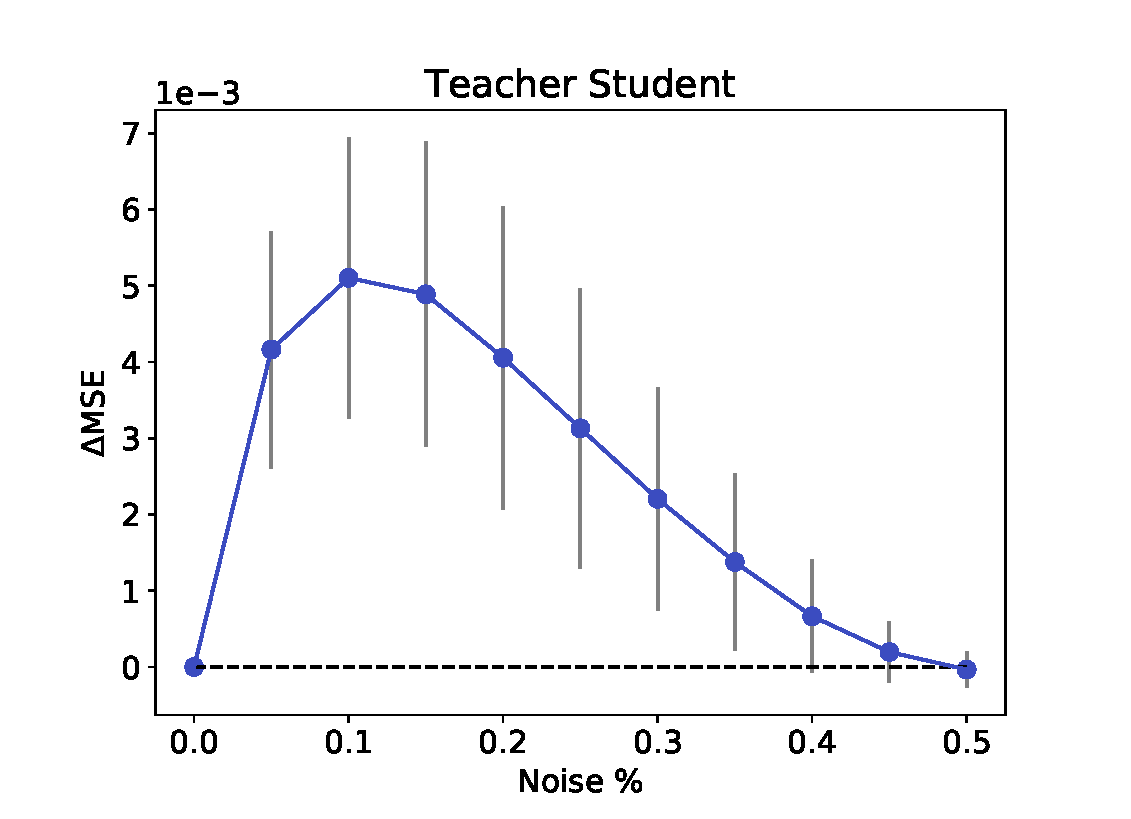
\includegraphics[width=1.1\linewidth]{figures/chapter3/delta_noise.eps}
    \caption{$\Delta\text{MSE} = \text{MSE}(classical) - \text{MSE}(quantum)$ versus the percentage of labels flipped in the training data. Error bars indicate the standard deviation over the 100 different runs. If the amount of noise is $0\%$, the classical and quantum perceptron will converge to the same solution. If the amount of noise is $50\%$ then both models cannot learn anything. Between these two points lies an area where the quantum perceptron has a lower MSE.} 
    \label{fig:lh_diff_mz}
\end{figure}

\section{Extensions}

While the results for simple data sets are promising, the quantum perceptron appears to have some limitations. We will discuss and resolve these problems in the next few sections by extending the initial model. A quantitative analysis will be left out for these extensions, but we will consider some toy problems to investigate the qualitative properties.

\subsection{Continuous Data}

The definition of $b(\mathbf{x})$ in equation \ref{eq:bx_rewritten} is problematic for continuous data, since $b(\mathbf{x})$ will always be $\pm1$ due to no overlapping samples occurring. This means that we always end up with the limiting case $m^x\to0$, logistic regression. To still be able to use $m^x$ we define a different $b(\mathbf{x})$ statistic for continuous data, that is dependent on the distance between samples.\newline

\noindent To start of, we rewrite the first term in the gradient rule for $\vecwk{z}$ as
\begin{align*}
    \sum_{\mathbf{x}} q(\mathbf{x})  b(\mathbf{x})\mathbf{x} &= \sum_{\mathbf{x}} q (2 q(y=1|\mathbf{x}) - 1) \mathbf{x}, \\ 
    \text{Bayes' Rule } &\rightarrow \sum_{\mathbf{x}} \frac{q(y=1| \mathbf{x})q(\mathbf{x})}{q(y=1)}\mathbf{x} = \sum_{\mathbf{x}}q(\mathbf{x} | y=1) \mathbf{x}\\
    &= \left(\sum_{\mathbf{x}} 2q(\mathbf{x} | y=1) q(y=1)\mathbf{x}\right) - \mathbb{E}[\mathbf{x}]_{q}\\
    &= 2 q(y=1) \mathbb{E}[\mathbf{x}|y=1]_{q} - \mathbb{E}[\mathbf{x}]_{q}.
\end{align*}
For the $\vecwk{x}$ gradient the we have to deal with the square root:
\begin{align}
    &= \sum_{\mathbf{x}} q(\mathbf{x})\mathbf{x} \sum_y  \sqrt{1-b(\mathbf{x})^2}\nonumber \\
    &= \sum_{\mathbf{x}} q(\mathbf{x})\mathbf{x} \sum_y \frac{1}{2} \sqrt{q(y=1|\mathbf{x})q(-y=1|\mathbf{x})}\nonumber.
\end{align}
By again using Bayes' rule and noticing the symmetry $y\Leftrightarrow-y$ we get
\begin{align}
    &= \sum_{\mathbf{x}} q(\mathbf{x}) \sqrt{1-b(\mathbf{x})^2} \mathbf{x}\nonumber ,\\
    &=\sum_{\mathbf{x}} q(\mathbf{x})2 \sqrt{q(y=1|\mathbf{x})q(y=-1|\mathbf{x})}\mathbf{x}  \nonumber\\
    \text{Bayes Rule} &\rightarrow \sum_{\mathbf{x}} 2 q(\mathbf{x}) \sqrt{\frac{q(y=1)q(\mathbf{x} | y=1)}{q(\mathbf{x})}}  \times \sqrt{\frac{q(y=-1)q(\mathbf{x} | y=-1)}{q(\mathbf{x})}}  \mathbf{x}\nonumber\\
    & = \sqrt{q(y=1)(1-q(y=1))} \times \sum_{\mathbf{x}} 2 \sqrt{q(\mathbf{x} | y=1)q(\mathbf{x} | y=-1)}\mathbf{x} \nonumber\\
    &= 2 \sqrt{q(y=1)(1-q(y=1))} \mathbb{E}[\mathbf{x}]_{Q},
    \label{eq:bx_rewritten}
\end{align}
with $Q(\mathbf{x}) = \sqrt{q(\mathbf{x} | y=1)q(\mathbf{x} | y=-1)}$. The new update rules are then given by
\begin{align*}
    \frac{\partial \mathcal{L}}{\partial \vecwk{x}} &= 2\sqrt{q(y=1)(1-q(y=1))} \mathbb{E}[\mathbf{x}]_{Q} - \sum_{\mathbf{x}} q(\mathbf{x})\tanh{h} \frac{h^x}{h}\mathbf{x},\\
    \frac{\partial \mathcal{L}}{\partial \mathbf{w}^y} &= -\sum_{\mathbf{x}} q(\mathbf{x}) \tanh{h} \frac{h^y}{h} \mathbf{x},\\
    \frac{\partial \mathcal{L}}{\partial \mathbf{w}^z} &= 2 q(y=1) \mathbb{E}[\mathbf{x}|y=1]_{q} - \mathbb{E}[\mathbf{x}]_{q} - \sum_{\mathbf{x}} q(\mathbf{x}) \tanh{h} \frac{h^z}{h} \mathbf{x}.
\end{align*}
Both gradients are now dependent on the expectation value of $\mathbf{x}$ given $y$, instead of the other way around. This allows us to introduce a kernel for $q(\mathbf{x}|y)$ in the input space that assigns a probability to $\mathbf{x}$ based on nearby samples with the same labels. Assume that we have data $\mathbf{x}\in \mathbb{R}^d$ and $y \in \{1, -1\}$. We place a multivariate Gaussian of fixed variance over each data point and then we calculate the conditional probability for a sample $\mathbf{x}$ of length $d$,
\begin{align*}
    &q(\mathbf{x} | y) = \frac{1}{Z}\sum_{\mathbf{x}^\prime} \mathds{I}(y^\prime = y) f(\mathbf{x}, \mathbf{x}^\prime; \Sigma)\\ &=\frac{1}{Z}\sum_{\mathbf{x}^\prime} \frac{\mathds{I}(y^\prime = y) }{\sqrt{(2 \pi)^d |\Sigma|}} \exp{-\frac{(\mathbf{x}^\prime - \mathbf{x})^T\Sigma^{-1}(\mathbf{x}^\prime - \mathbf{x})}{2}},
\end{align*}
where $Z$ ensures that $\sum_{\mathbf{x}} q(\mathbf{x} | y) = 1$. If we set all covariances zero and the variances to $\sigma^2$, we get $\Sigma = \sigma^2 \mathbb{1}$ which simplifies the above expression to
\begin{align*}
    = \frac{1}{Z}\sum_{\mathbf{x}^\prime} \frac{\mathds{I}(y^\prime = y) }{\sqrt{(2 \pi \sigma^2)^d }} \exp{-\frac{(\mathbf{x}^\prime - \mathbf{x})^T(\mathbf{x}^\prime - \mathbf{x})}{2\sigma^2}}.
\end{align*}
Because we place a Gaussian over each point $\mathbf{x}$, we have to correct the distribution $q(\mathbf{x})$ accordingly,
\begin{align*}
    q(\mathbf{x}) = \sum_y q(y)q(\mathbf{x}|y) =  \sum_y q(y)\frac{1}{Z}\sum_{\mathbf{x}^\prime} \mathds{I}(y^\prime = y) f(\mathbf{x}; \mathbf{x}^\prime, \sigma^2 \mathbb{1}).
\end{align*}
The resulting probability landscapes can be seen in figure \ref{fig:gaussian_landscape}
\begin{figure}[htb!]
    \centering
    \makebox[\textwidth][c]{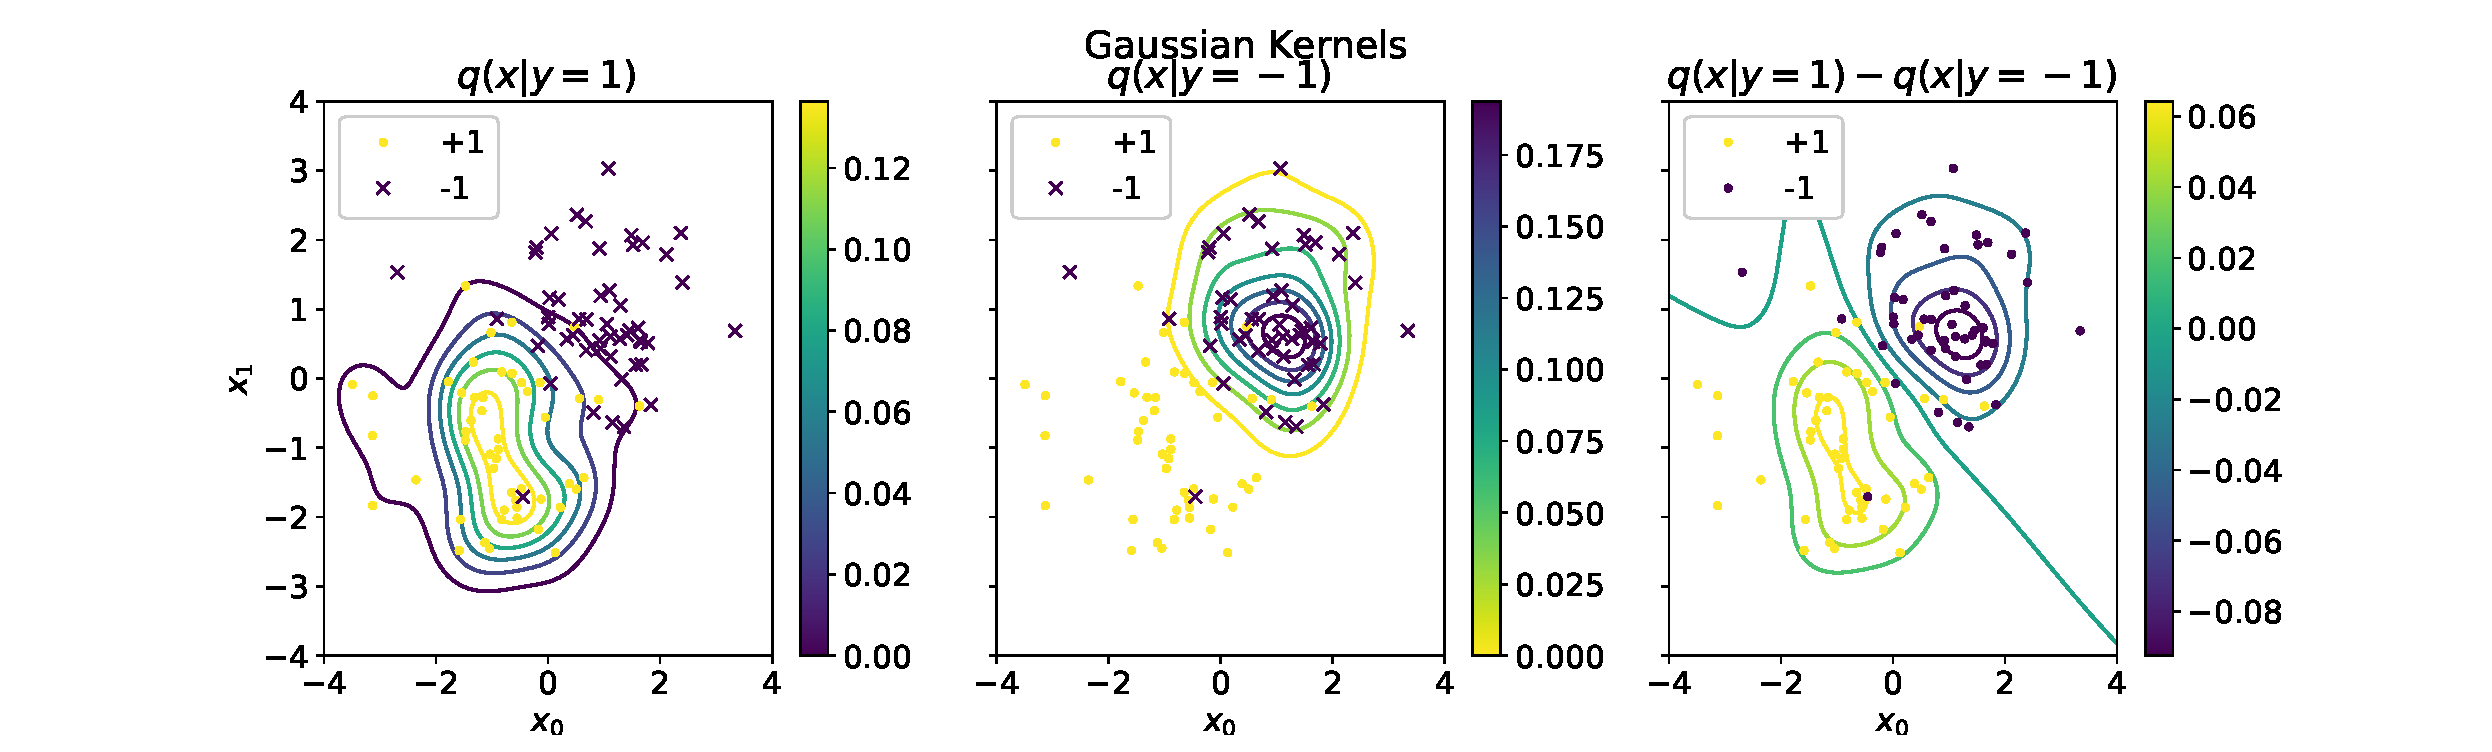
\includegraphics[width=1.5\textwidth]{figures/chapter3/gauss.eps}}
    \caption{Gaussian landscapes for $\sigma^{\prime 2} = 0.25$ for two random data sets. In the left panel we see the probability of finding a sample with label $y=1$ in the input space. In the middle we have the same figure but now for $y-1$. The expectation value for finding the sample with a certain label is plotted in the right panel.}
    \label{fig:gaussian_landscape}
\end{figure}{}
If the distributions over the samples overlap, then $ \mathbb{E}[\mathbf{x}]_{Q} \neq 0$ and as a result $\vecwk{x}$ becomes non-zero. We thus measure the impact of neighbouring samples on the likelihood of observing a sample within a certain class. If the samples are far apart, then we require broad distributions to create overlap between samples. \newline 

\noindent To test this model we create $N$ samples of length $d=2$ where $X_1\sim \mathcal{N}(\bm{\mu}_1,\sigma^2 \mathbb{1})$ with label $y=1$ and $N$ samples $X_2\sim \mathcal{N}(\bm{\mu}_2, \sigma^2 \mathbb{1})$ with label $y=-1$. $\sigma^2 = 0.5$. $\bm{\mu}_1 = (-1,-1)$ and $\bm{\mu}_2 = (0,0)$. We generate $100$ samples for each label and set $\epsilon=0.01$. We set the variance of the sample Gaussians in $q(\mathbf{x} | y)$ to $\sigma^{\prime 2} = 0.05$. The shape of the separation boundary is very sensitive to asymmetries in the distributions. If the data for both labels is distributed equally, and there are an equal number of samples with label $y=1$ as there are with $y=-1$, then we get a straight boundary through the data, since the distance based kernel cancels everywhere. If $q(\mathbf{x} | y)\in \{0,1\}$, so only sharp peaks around the samples, then $\vecwk{x}\rightarrow 0$ and we get a thin straight line as boundary, just as in the classical case. However, if there are asymmetries in the data we observe the wavering effect of section \ref{sec:results}, as can be seen in figure \ref{fig:boundary_cont}.\newline

\noindent The cost function is changed as a result of the continuous kernel and this affects the placement of the boundaries. However, the probability boundaries retain the same shapes as in section \ref{sec:probs}, since the only thing affected is the data density matrix. The model $\rho_\mathbf{x}$ still has the same degrees of freedom as before and thus retains the same properties as before. The introduction of the Gaussian kernels introduces an extra parameter, namely the variance $\sigma^{\prime 2}$. This introduces a bias in the algorithm. We either need to set it before training or adapt it during learning for optimal performance. This was not further explored here, since we only wanted to show the qualitative properties of the continuous model. In the end, the quantum perceptron retains its functionality in dealing with better noisy data, at the cost of introducing an additional free parameter.

\begin{figure}[htb!]
    \centering
    \makebox[\textwidth][c]{
        \subfloat[]{%
            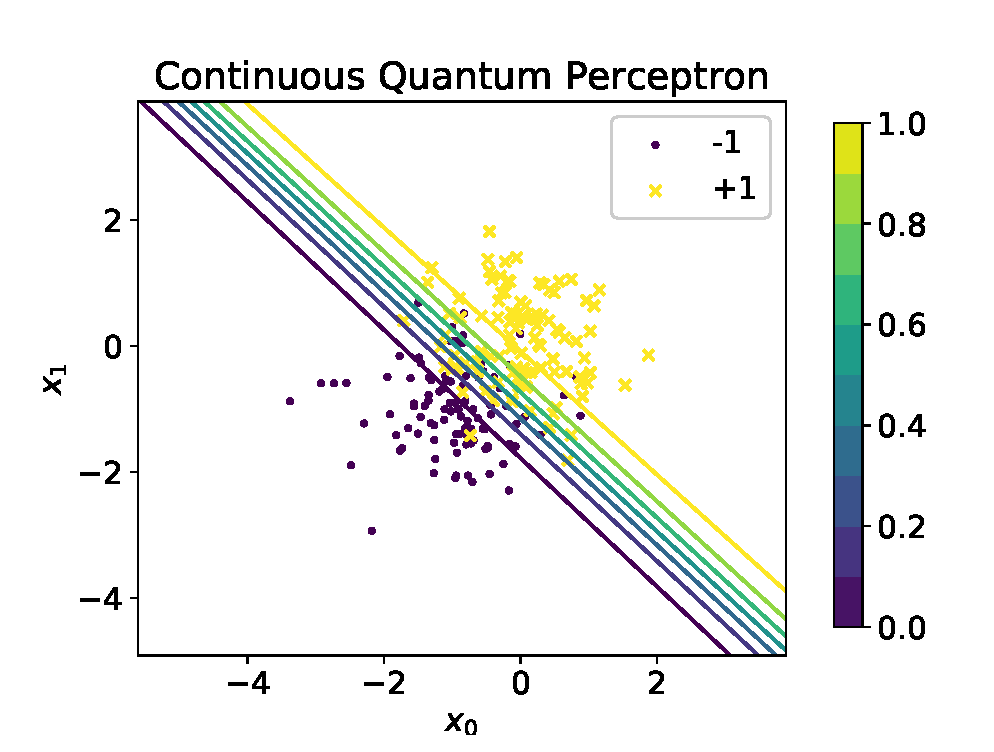
\includegraphics[clip,width=0.7\columnwidth]{figures/chapter3/cont_1.eps}
        }
        \subfloat[]{%
            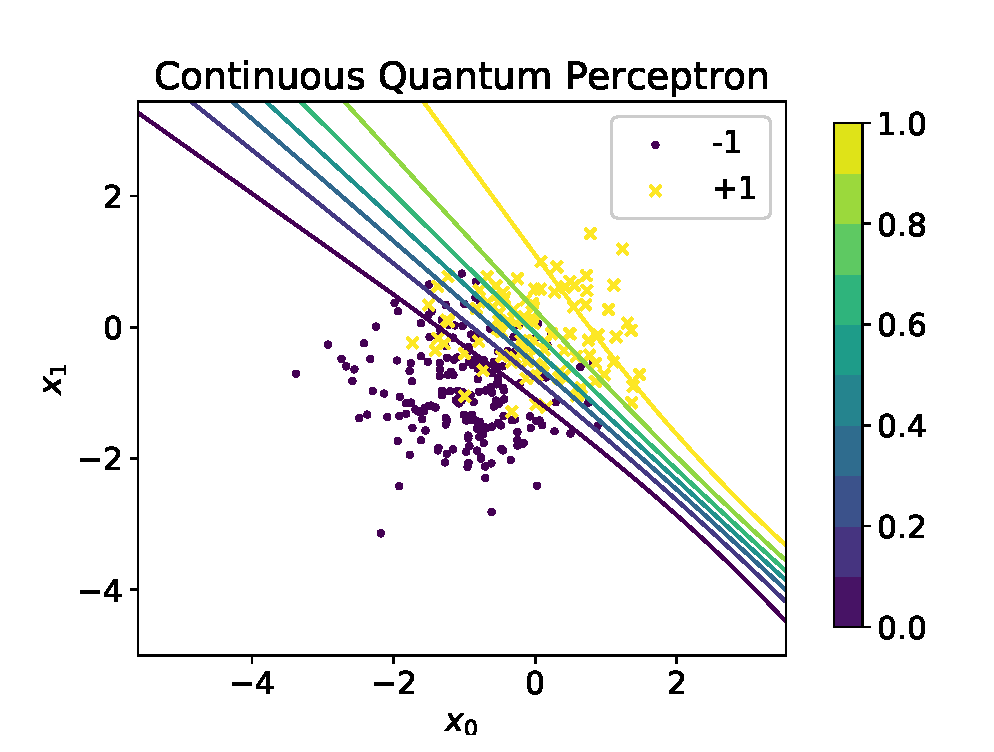
\includegraphics[clip,width=0.7\columnwidth]{figures/chapter3/cont_2.eps}
        }
    }    \caption{Quantum perceptron for continuous data. On the left side the number of samples between the two classes is equal ($n=100$). The kernels functions average out and the separation boundary is symmetric with respect to the two distributions. If we double the number of samples for the $-1$ class the asymmetry in the data causes the star like separation boundaries to appear.}
    \label{fig:boundary_cont}
\end{figure}

\clearpage
\subsection{Multiple Classes}

The classical perceptron is inherently a binary classifier, but can be extended to allow for multiclass regression.
The model probability distribution for a multinomial logistic regression or maximum entropy classifier is given by \cite{Murphy2012},
\begin{equation}
    p(y=c|\mathbf{x}, (\mathbf{w}_1,\ldots,\mathbf{w}_{C})) = p(y=c|\mathbf{x}, \mathbf{W}) = \frac{\exp(\mathbf{w}_c\cdot\mathbf{x})}{\sum_{c^\prime}^C \exp(\mathbf{w}_{c^\prime}\cdot\mathbf{x})} = \mathcal{S}_{c}^\mu \label{eq:multiclass_reg}.
\end{equation}
For $C$ classes $c\in \{0,1,\ldots,C-1\}$ where we adopt Murphy's capital letter notation for matrices, where $ \mathbf{W}$ is a matrix with columns equal to $\mathbf{w}_i$. The output $y$ is one-hot encoded by a vector $\mathbf{y}^\mu$ where the c-th bit is turned on if and only if $y= c$. By using Lagrange Multipliers we can show that this distribution maximizes the classical entropy (See appendix \ref{sec:entanglement}) \cite{Jaynes1957}. Plugging equation \ref{eq:multiclass_reg} into the classical likelihood gives
\begin{align*}
    f(\mathbf{W}) &= -\sum_{\mathbf{x}}^N \sum_c^{C-1} y_c \log p(y=c|\mathbf{x}, \mathbf{W})\\
    &=-\sum_{\mathbf{x}}^N \left(\left(\sum_c^{C-1} y_c \mathbf{w}_c\cdot\mathbf{x} \right) - \log\left( \sum_{c^\prime}^{C-1} \exp(\mathbf{w}_{c^\prime}\cdot\mathbf{x})\right)\right).
\end{align*}
Clearly, a gradient with respect to a set of weights $\mathbf{w}_c$ gives 
\begin{equation*}
    \nabla_{\mathbf{w}_c} f(\mathbf{W})  = \sum_{\mathbf{x}} (\mathcal{S}_{c}^\mu - y_c)\mathbf{x}.
\end{equation*}
If we look at the softmax function we see that it is actually fully determined by $C-1$ sets of weights, due to the fact the probability must sum to 1. By shifting all weights with a constant vector $\mathbf{d}$ we get
\begin{equation*}
    \frac{\exp((\mathbf{w}_c - \mathbf{d})\cdot\mathbf{x})}{\sum_{c^\prime}^{C-1} \exp((\mathbf{w}_{c^\prime}- \mathbf{d})\cdot\mathbf{x})} = \frac{\exp(-\mathbf{d}\cdot\mathbf{x})\exp(\mathbf{w}_c\cdot\mathbf{x})}{\exp(-\mathbf{d}\cdot\mathbf{x})\sum_{c^\prime}^{C-1} \exp(\mathbf{w}_{c^\prime}\cdot\mathbf{x})} = \frac{\exp(\mathbf{w}_c\cdot\mathbf{x})}{\sum_{c^\prime}^{C-1} \exp(\mathbf{w}_{c^\prime}\cdot\mathbf{x})}.
\end{equation*}
If we set $\mathbf{d} = \mathbf{w}_C$, we eliminate one set of parameters. If $C=2$ we retrieve the original description of logistic regression,
\begin{equation*}
     \mathcal{S}^\mu = \frac{\exp(\mathbf{w}\cdot\mathbf{x})}{1 + \exp(\mathbf{w}\cdot\mathbf{x})} = \frac{1}{1 + \exp(-\mathbf{w}\cdot\mathbf{x})}.
\end{equation*}
In order to extend this multinomial regression to the quantum likelihood description, we need to find a density matrix model that is analogous to the maximum entropy ansatz for a classical system. As with the quantum perceptron, we use the quantum mechanical canonical ensemble ansatz for the density matrix,
\begin{equation}
    \rho_\mathbf{x} = \frac{\exp(H)}{\Tr{\exp(H)}} \label{eq:density_su3},
\end{equation}
which reduces to the Boltzmann distribution if $H$ contains no off-diagonal elements and diagonal elements corresponding to the Boltzmann probabilities. Up to this point, we considered models where the output state was a qubit, so $\dim(H)=2$ and a general basis for $H$ was given by the Pauli basis $\sum_k h^k \sigma^k$. From group theory we know that this is the fundamental representation of the $\text{SU}(2)$ Lie Algebra, and a basis for $2\times2$ traceless Hermitian matrices. For multinomial regression we can look at a description of the data in terms of the representation of the Lie algebra of $\text{SU}(N)$ , where $N=C$ is the number of different classes in the data. Let us start with $C=3$ classes, which describes a 3 level system called a qutrit \cite{Nisbet-Jones2013}. We have to note that this is not a description of a boson, because bosons are described by the adjoint representation \textbf{3} of $\text{SU}(2)$, which does not span the full space of density matrices. The group $\text{SU}(3)$ is used in quantum chromodynamics to describe the symmetry of quark colors \footnote{Maybe one day we will have quantum chromo computers, capable of manipulating quark colors.}. \newline

\noindent The fundamental representation of $\text{SU}(3)$ is given by the so called Gell-Mann matrices, a set of 8 linearly independent $3\times3$ matrices that span the full space of traceless Hermitian $3\times 3$ matrices. They are given by
\begin{align*}
    \lambda^1 &= 
    \begin{pmatrix}
    0 & 1 & 0 \\
    1 & 0 & 0\\
    0 & 0 & 0
    \end{pmatrix},
    \quad
    \lambda^2 = 
    \begin{pmatrix}
    0 & -i & 0 \\
    i & 0 & 0\\
    0 & 0 & 0
    \end{pmatrix},
    \quad
    \lambda^3 = 
    \begin{pmatrix}
    1 & 0 & 0 \\
    0 & -1 & 0\\
    0 & 0 & 0
    \end{pmatrix},\\
    \lambda^4 &= 
    \begin{pmatrix}
    0 & 0 & 1 \\
    0 & 0 & 0\\
    1 & 0 & 0
    \end{pmatrix},
    \quad
    \lambda^5 = 
    \begin{pmatrix}
    0 & 0 & -i \\
    0 & 0 & 0\\
    i & 0 & 0
    \end{pmatrix},\\
    \lambda^6 &= 
    \begin{pmatrix}
    0 & 0 & 0 \\
    0 & 0 & 1\\
    0 & 1 & 0
    \end{pmatrix},
    \quad
    \lambda^7 = 
    \begin{pmatrix}
    0 & 0 & 0 \\
    0 & 0 & -i\\
    0 & i & 0
    \end{pmatrix},
    \quad
    \lambda^8 = \frac{1}{\sqrt{3}}
    \begin{pmatrix}
    1 & 0 & 0 \\
    0 & 1 & 0\\
    0 & 0 & -2
    \end{pmatrix}.
\end{align*}
Using these matrix we can write a general three state Hamiltonian $H$ as
\begin{equation*}
    H = \sum_k h^k\lambda^k
\end{equation*}
with $h^k=\mathbf{x}\cdot\mathbf{w}^k$ as before. Remember that for the Pauli matrices we had the following convenient expression:
\begin{equation*}
    \exp{{ia(\hat{n}\cdot\bm{\sigma})}} = \mathbb{1} \cos{a} + i(\hat{n}\cdot\bm{\sigma}) \sin{a},
\end{equation*}
with $|\Hat{n}|=1$ and $a\in \mathbb{R}$. By proving this expression we will discover a problem related to the $\text{SU}(3)$ (and more generally $\text{SU}(N)$) descriptions of the density matrix model. The proof relies on the fact that $(\hat{n}\cdot\bm{\sigma})^{2p}=\mathbb{1}$, for $p=1$ we have
\begin{align*}
    (\hat{n}\cdot\bm{\sigma})^2 &= (n^x \sigma^x + n^y \sigma^y + n^z \sigma^z)^2 \\
    &+ n^y n^z\sigma^y  \sigma^z + n^z n^x\sigma^z  \sigma^x +n^z n^y \sigma^z  \sigma^y + n^z n^z  \sigma^z \sigma^z\\
    &= (n^x)^2 (\sigma^x)^2 + (n^y)^2 (\sigma^y)^2  + (n^z)^2 (\sigma^z)^2 \\
    &+  n^x n^y(\sigma^x  \sigma^y + \sigma^y  \sigma^x) + n^x n^z(\sigma^x  \sigma^z + \sigma^z  \sigma^x) + n^y n^z(\sigma^y  \sigma^z + \sigma^z  \sigma^y)\\
    & = \mathbb{1}\left((n^x)^2 + (n^y)^2  + (n^z)^2 \right)+ n^x n^y\{\sigma^x, \sigma^y\} + n^x n^z\{\sigma^x, \sigma^z\} + n^y n^z\{\sigma^y, \sigma^z\}\\
    & = \mathbb{1},
\end{align*}
where we used that $\{\sigma_i, \sigma_i\} = 2I$ and $\{\sigma_i, \sigma_j\}=0$ for $i\neq j$. If we write out the exponential operator we get
\begin{align}
    \exp{{ia(\hat{n}\cdot\bm{\sigma})}} &= \sum_{k=0}^\infty \frac{i^k((a\hat{n}\cdot\bm{\sigma})^k)}{k!} = \sum_{p=0}^\infty \frac{(-1)^p(a\hat{n}\cdot\bm{\sigma})^{2p})}{2p!} + i\sum_{q=0}^\infty \frac{(-1)^q(a\hat{n}\cdot\bm{\sigma})^{2q+1})}{(2q+1)!}\nonumber\\
    & = \sum_{p=0}^\infty \frac{(-1)^p(a\hat{n}\cdot\bm{\sigma})^{2p}}{2p!} + i(\hat{n}\cdot\bm{\sigma})\sum_{q=0}^\infty \frac{(-1)^q a^{2q+1}(\hat{n}\cdot\bm{\sigma})^{2q}}{(2q+1)!}\nonumber\\
     &=  \mathbb{1} \sum_{p=0}^\infty \frac{(-1)^p a^{2p}}{2p!} + i(\hat{n}\cdot\bm{\sigma})\sum_{q=0}^\infty \frac{(-1)^q a^{2q+1})}{(2q+1)!}\nonumber\\
     & = \mathbb{1} \cos{a}+ i(\hat{n}\cdot\bm{\sigma})\sin{a} \label{eqn:exp_pauli}.
\end{align}
For $\exp{{a(\hat{n}\cdot\bm{\sigma})}}$ we replace the sine and cosine with their respective hyperbolic functions. For the quantum perceptron this relation meant that we could easily find the derivatives of the likelihood function, but this seems to be a property of $\text{SU}(2)$ alone. The commutation relations of $\text{SU}(3)$ are
\begin{align*}
    \left(\frac{\lambda^a}{2}, \frac{\lambda^b}{2}\right) &=  i \sum_{c=1}^8 f^{abc} \frac{\lambda^c}{2},\\
    \left\{\frac{\lambda^a}{2}, \frac{\lambda^b}{2}\right\} & \neq 0,
\end{align*}
with $f^{abc}$ the structure constant of $\text{SU}(3)$. This means that $(\hat{n}\cdot\bm{\lambda})^{2p} \neq 1$ and that there is no easy way to represent the exponent in a similar fashion as in equation \ref{eqn:exp_pauli}. Some work has been done to come up with such a formula nonetheless, but it is not as elegant as for the $2\times2$ case, and hard to generalize to $\text{SU}(N)$ \cite{Curtright2015}. This means that we will have to calculate the gradient numerically. The quantum likelihood is given by
\begin{equation*}
    g(\mathbf{W}) = \sum_{\mathbf{x}} q(\mathbf{x}) \Tr{\eta_\mathbf{x} \log \rho_\mathbf{x}},
\end{equation*}
and the model is given by equation \ref{eq:density_su3}. In order to calculate the log of the trace we have to determine the eigenvalues of $H$:
\begin{align*}
    \log\left(\frac{\exp(H)}{\Tr{\exp(H)}}\right) &= \log(\exp(H)) - \log(\Tr{\exp(H)}) = H - \log(\sum_i \exp(\lambda_i)).
\end{align*}
So numerically determining the eigenvalues of H will give us a value for quantum log-likelihood.
Coming up with an analytic expression for the eigenvalues will be quite cumbersome, so we will have to resort to a numerical method to determine them. The data density matrix can be constructed similarly as for the qubit by writing the data as a wave function,
\begin{align*}
    \ket{\psi} &= \sqrt{q(y=0|\mathbf{x})}\ket{0} + \sqrt{q(y=1|\mathbf{x})}\ket{1} + \sqrt{q(y=2|\mathbf{x})}\ket{2}\\
    \eta_\mathbf{x} &= \ket{\psi}\bra{\psi}.
\end{align*}
We determine the gradient with respect to each weight $w_i$ numerically by calculating
\begin{equation*}
    \nabla_{\mathbf{w}_i} g(\mathbf{W})  = \frac{g(\mathbf{w}_i + \epsilon | \mathbf{w}_j ) - g(\mathbf{w}_1,\ldots,\mathbf{w}_8 ) }{\epsilon},
\end{equation*}
for $j\in\{1,\ldots,8\}$ and $j\neq i$. Update the weights as
\begin{equation*}
    \mathbf{w}_i^{t+1} = \mathbf{w}_i^{t} - \epsilon \nabla_{\mathbf{w}_i} g(\mathbf{W}^t).
\end{equation*}
Again, we are faced with the question of how to determine a probability. For the binary problem, the expectation value $\expval{\sigma^z}=m^z$ gave us a value between $-1$ and $1$, allowing for an easy mapping to a probability $p(y|\mathbf{x};\mathbf{w})\in[0,1]$. Measuring one of the $\lambda^k$ operators would give a scalar field that we would have to map to a probability, but there is no clear way of how to do this. A method that also generalizes to $C$ class perceptrons is taking the diagonal elements of $\rho_\mathbf{x}$. If the model density matrix contains no off-diagonal elements, these would correspond to the class probabilities of the classical multinomial logistic regression. Taking $m^z$ for constructing a probability for the qubit quantum perceptron is equivalent to taking the diagonal elements as probabilities. With this in mind, we choose the diagonal elements of $\rho_\mathbf{x}$ as the class probabilities,
\begin{align*}
    p(y=c|\mathbf{x};\mathbf{w}) = \rho_{c,c}.
\end{align*}
As before, we observe that the off-diagonal elements go to zero if there is no noise in the data, since $\eta_\mathbf{x}$ will contain no off diagonal elements as well. From figure \ref{fig:qm_mn_r} we observe this behaviour and retrieve the spread out probability boundaries for a 3 class problem.

\begin{figure}[htb!]
    \centering
    \makebox[\textwidth][c]{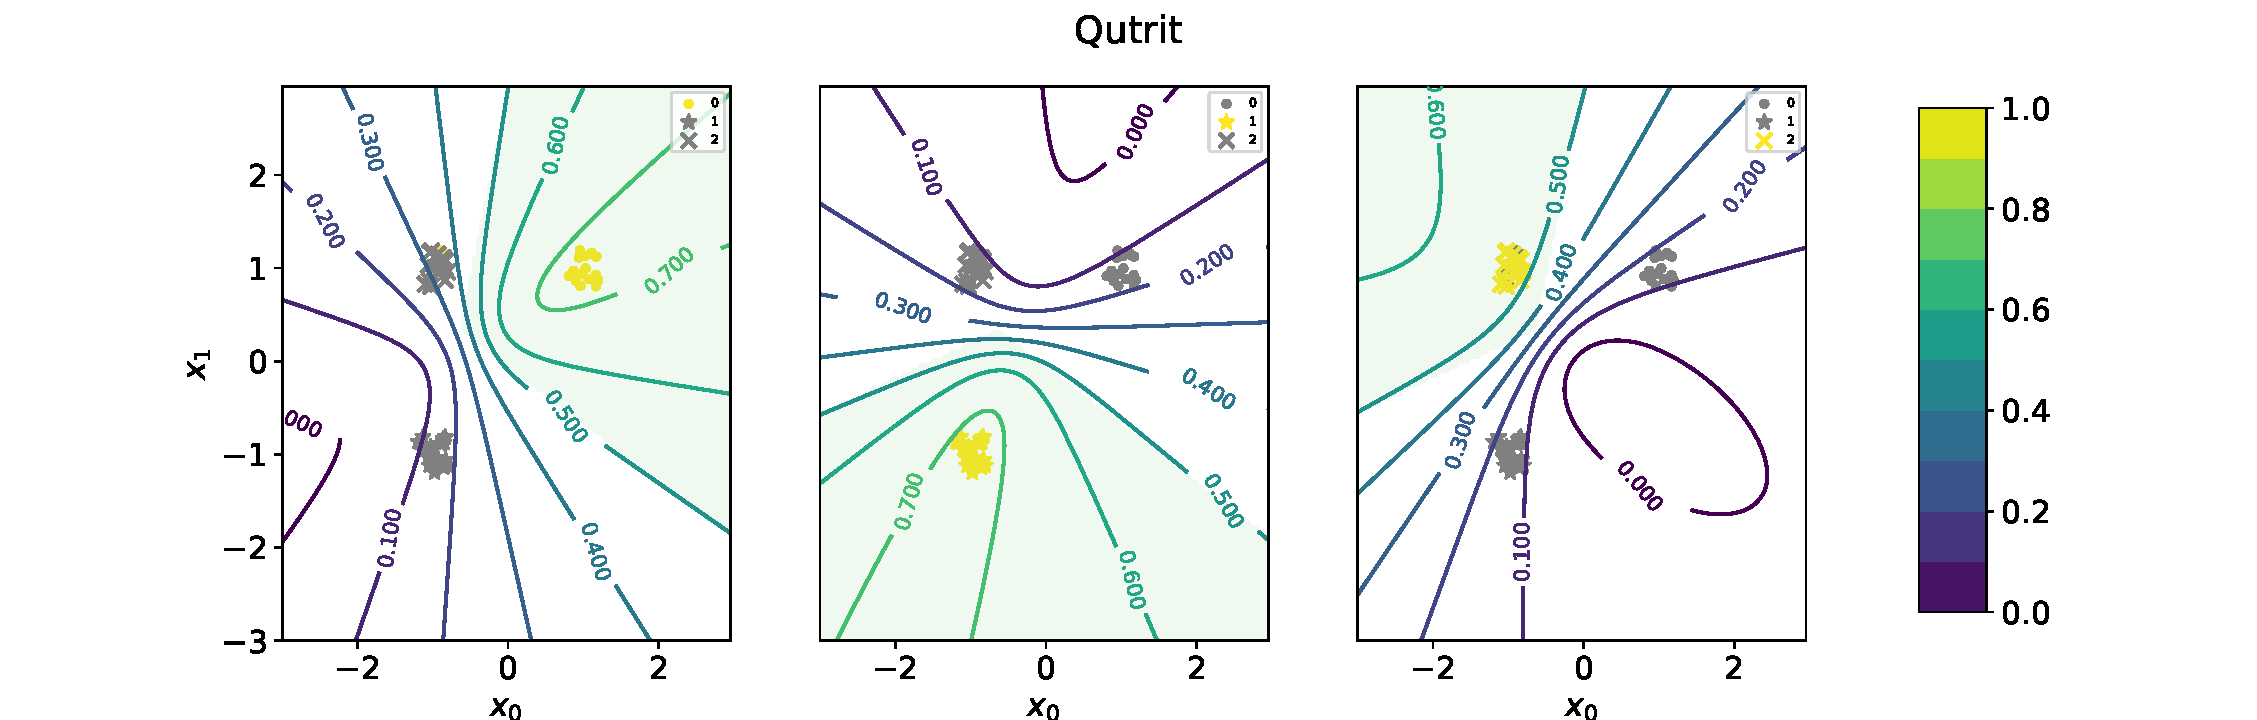
\includegraphics[width=1.6\textwidth]{figures/chapter3/qutrit.pdf}}
    \caption{Separation boundaries of qutrit perceptron for noisy data. The contours show the probabilities $p(y=c|\mathbf{x};\mathbf{w})$. The yellow icon in the legend indicates the class $c$. The light green background indicates the area in the input space where $p(y=c|\mathbf{x};\mathbf{w})$, so where we would predict class $c$ . For $30\%$ of the outputs of the samples $\mathbf{x} = (-1,1)$ we assign label $0$. The wavering effect of the probability boundaries that we saw for the binary case returns.}
    \label{fig:qm_mn_r}
\end{figure}

\clearpage

\noindent The idea of qutrit regression is easily extended to a qudits perceptron. A qudit is the generalization of a two-level system to an $d$-level system. For $\text{SU}(C)$, the number of matrices that are required to span the full space is equal to $C^2-1$, which can be constructed with the following rules \cite{Bertlmann2008}:
\begin{enumerate}
    \item Symmetric matrices\\
    \begin{align*}
        \Gamma^{jk}_{sym} = \ketbra{j}{k}+\ketbra{k}{j}, \quad 1\leq j<k\leq C
    \end{align*}
        \item Antisymmetric matrices \\
    \begin{align*}
        \Gamma^{jk}_{asym} = -i\ketbra{j}{k}+i\ketbra{k}{j}, \quad 1\leq j<k\leq C
    \end{align*}
            \item Diagonal matrices \\
    \begin{align*}
        \Gamma^{l}_{diag} = \sqrt{\frac{2}{l(l+1)}}\left(\sum^l_{j=1}\ketbra{j}{j}-l\ketbra{l+1}{l+1}\right), \quad 1\leq j\leq C-1
    \end{align*}
\end{enumerate}
With these simple rules we can extend out quantum perceptron model to any number of classes. An example solution for $C=6$ is shown in figure \ref{fig:qm_mn_5}.
\begin{figure}[htb!]
    \centering
    \makebox[\textwidth][c]{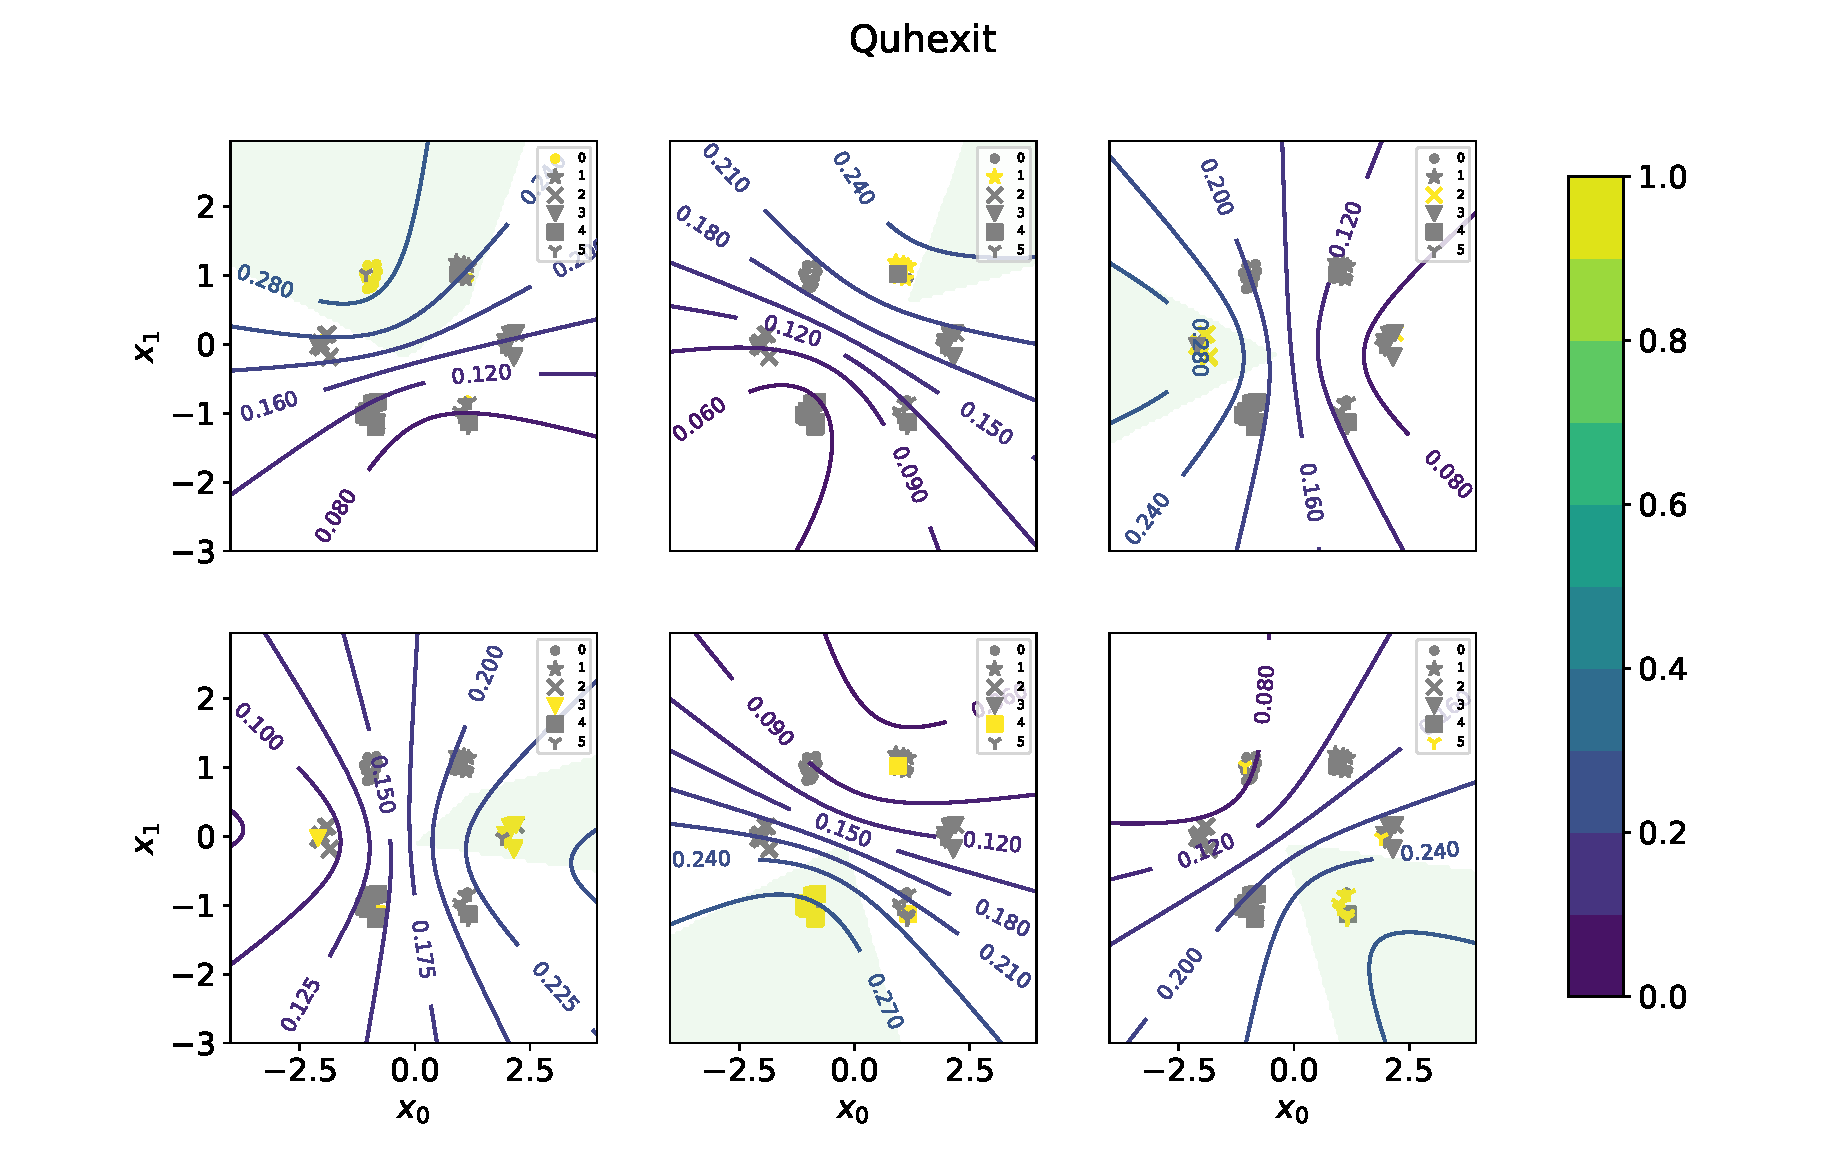
\includegraphics[width=1.6\textwidth]{figures/chapter3/quhexit.pdf}}
    \caption{Separation boundaries of qudit perceptron for noisy data arranged in a hexagon. The contours show the probabilities $p(y=c|\mathbf{x};\mathbf{w})$. The yellow icon in the legend indicates the class $c$. The light green background indicates the area in the input space where $p(y=c|\mathbf{x};\mathbf{w})$, so where we would predict class $c$. Additioally, $30\%$ of the labels are randomly exchanged between the samples. The flipped labels perturb the boundaries as expected.}
    \label{fig:qm_mn_5}
\end{figure}
\noindent The quantum perceptron can be extended to learn multiclass classification problems, but this comes at the cost of a significant performance decrease. Although learning $C^2-1$ vector weights in not a problem, we have to find the eigenvalues of each $C\times C$ density matrix for each sample $\mathbf{x}$ at each training step in order to calculate $\log{\sum_i \exp(\lambda_i)}$. Consider the MNIST data set, a collection of $60000$ handwritten digits from $0-9$ of size $28\times28$. In order for the perceptron to learn this data we would have to diagonalize $60000$ $10\times 10$ matrices at each training step and update $(10^2 - 1 )=99$ vectors. Compare this to the classical perceptron, which only has to calculate $\sum_{\mathbf{x}} (\mathcal{S}_{c}^\mu - y_c)\mathbf{x}$ for $9$ vectors weights and update them. However, the extra utility of the quantum perceptron might outweigh the increase in computational cost.

\clearpage
\subsection{Classical Limit}

Some of the work in this thesis was presented and discussed at the ``Bits and brains" meeting, an interdisciplinary seminar with different groups working on materials science and their possible applications to neuromorphic computing. With regards to the quantum perceptron, the following point was put forward: Since we are not using non-classical correlations or entanglement, we cannot talk experimentally of a quantum system. We are using a finite temperature description, and measuring this ensemble means the quantum properties of the system such as the superposition of states, might not be distinguishable from a non-quantum system due to thermal effects. We are thus not using quantum mechanics in any way and the qualitative properties can be achieved by considering a classical system. More specifically, simply measuring $m^x$ and $m^z$ is not enough to call it a quantum perceptron. It was suggested that a similar model might be obtained from a classical magnetic material. \newline

\noindent To analyze this argument we will attempt to replace $m^k$ with a classical magnetization function. The perfect candidate for this is the Langevin function, which links the applied magnetic field to the total magnetization of a paramagnetic material. See figure \ref{fig:paramag}. 
\begin{figure}[hb]
    \centering
    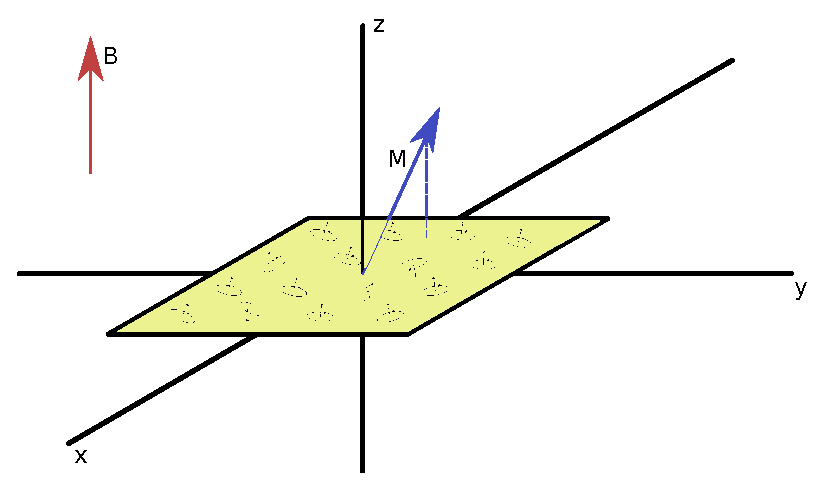
\includegraphics[width=\textwidth]{figures/chapter3/paramagnetism.eps}
    \caption{Magnetization in a paramagnetic material. Individual magnetic dipoles all contribute to the total magnetization in the material.}
    \label{fig:paramag}
\end{figure}
A paramagnetic material has permanent magnetic dipoles, even in the absence of an external magnetic field. In a uniform field these dipoles have a potential energy of
\begin{equation*}
    E = -\mathbf{m}\cdot\mathbf{B}.
\end{equation*}
If we consider the coordinate system where $\mathbf{m}$ lies in the $xz$-plane, we get $U = -mB \cos{\theta}$ with $\theta$ the angle between the two vectors in the $xz$-plane. The change in energy is given by $dE = mB\sin{\theta}d\theta$. If we assume that quantum effects are negligible then the number of states $N$ can be written with the Boltzmann distribution,
\begin{align*}
    N &= \int n(E) dE,\\
    \frac{dN}{dE} &= n(E) = \frac{1}{Z} \exp(-\beta E).
\end{align*}
Since this can be rewritten in terms of $\theta$, this is also the number of dipoles with a orientation between $\theta$ and $\theta+d\theta$. \newline

\noindent The total magnetization can be written as an integral over all N dipoles projected onto the direction of the applied magnetic field,
\begin{align*}
    M  &= \int_0^N m \cos{\theta} dn = N\langle m \rangle,\\
    \frac{\langle m \rangle}{m} &= \frac{1}{N} \int_0^N \cos{\theta} dn,\\
    N &\equiv \int_0^N dn,
\end{align*}
where $\langle m \rangle$ is the average magnetization in the direction of $\mathbf{B}$. Substituting 
\begin{align*}
    dn &= \frac{1}{Z}mB\sin{\theta} \exp[\beta mB\cos{\theta}]d\theta,\\
    x &=\beta mB\cos{\theta} = a \cos{\theta},\\
    d\theta &= -1 / a\sin{\theta} dx,
\end{align*}
gives
\begin{align*}
    \frac{\langle m \rangle}{m} &= \frac{\frac{1}{a}\int^a_{-a} x e^x dx}{\int^a_{-a} e^x dx}\\
    &= \frac{e^a + e^{-a}}{e^a - e^{-a}} - \frac{1}{a} = \frac{1}{\tanh{a}} - \frac{1}{a} \\
    &= L(a) = L(m).
\end{align*}
So $M=N m L(a)$ \cite{Lidzey2019}. This is the length of the magnetization vector, $\mathbf{M}$, which points in the same direction as the magnetic moment $\mathbf{m}$ so $\mathbf{M} =  N L(a) m \hat{\mathbf{m}} =  N L(a) \mathbf{m}$, since $\mathbf{m} =  \mathbf{M} V$ if the magnetization is constant across the magnet. Parametrizing $\mathbf{m} = \frac{\mathbf{h}}{h}$ with $h^k = \mathbf{w}^k\cdot \mathbf{x}$ and absorbing the constants in the weights gives a relation of the form
\begin{equation*}
    M^k = L(h) \frac{h^k}{h},
\end{equation*}
which is similar to the parametrization in equation \ref{eq:density_matrix_basis}, except the $\tanh$ is replaced by the Langevin function. Since $M^z \in [-1,1]$, we can define a probability $p(y|\mathbf{x};\mathbf{w}) = \frac{1}{2}(1+y M^z)$ that assigns a proper probability to a class $y$. For a physical realization we have to bring a material into a certain state and measure $M^x$ and $M^z$. If $M^z>0$, so the magnetization vector points in the positive $z$ direction, we assign class 1.  If $M^z<0$, we assign class 0. Depending on the norm, which is still $\sqrt{(h^x)^2+(h^z)^2}$, we introduce an uncertainty about this classification. Unlike with the quantum perceptron, the only purpose of $M^x$ is an additional degree of freedom to control the norm. $M^x$ is not inherently coupled to flipped labels. Another more obvious difference is that we do not have a hyperbolic tangent but a Langevin function to link the fields with the magnetization. Both functions  have a codomain of $(-1,1)$ and have a similar shape, as can be seen in figure \ref{fig:langevin}.
\begin{figure}[ht]
    \centering
    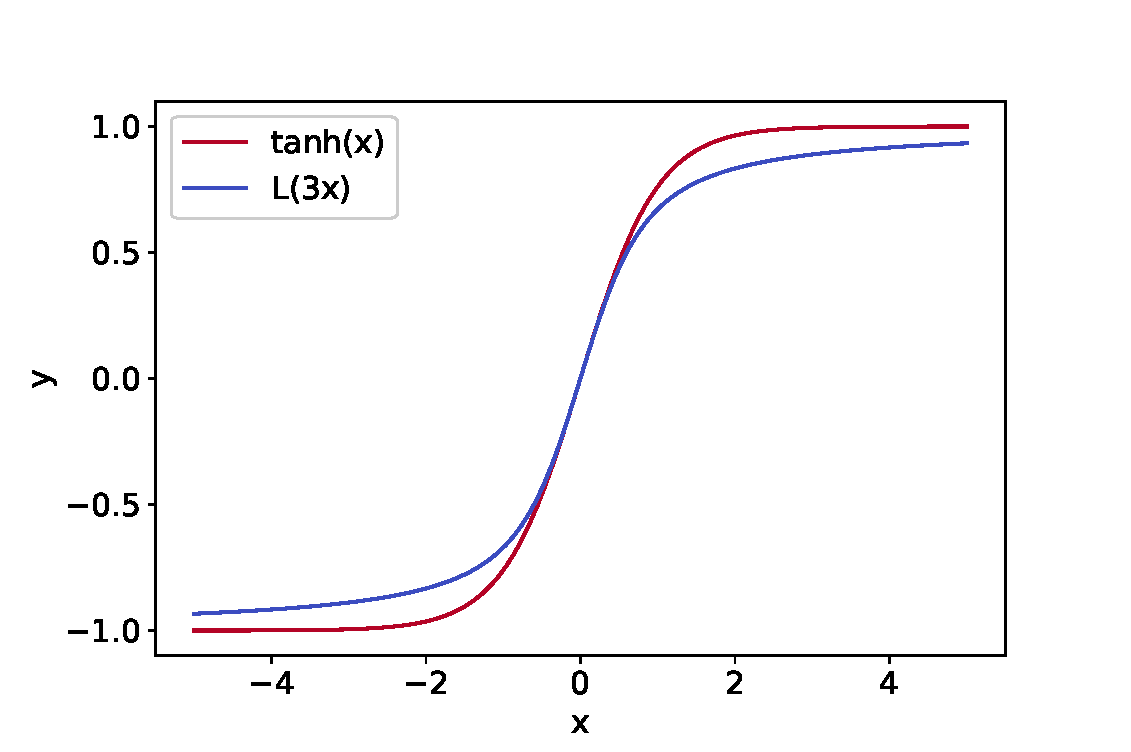
\includegraphics[width=\textwidth]{figures/chapter3/langevin_tanh.eps}
    \caption{Difference between Langevin function and $\tanh$. Multiplying the argument with 3 gives a function similar to $\tanh(x)$.}
    \label{fig:langevin}
\end{figure}
Also, we cannot just plug in a different nonlinear function in equation \ref{eq:grads}. These gradients are derived from an optimization criterion, the negative quantum log-likelihood. We have to rederive the gradient update rules from a new optimization criterion that incorporates this redefinition of the fields. To this end, define the likelihood
\begin{align*}
    \mathcal{L} = \sum_\mu q(\mathbf{x}) \sum_y q(y|\mathbf{x}) \log [\frac{1}{2}(1+y M^z)].
\end{align*}
Deriving this likelihood with respect to the weights $\mathbf{w}^k$, with $h^k = \mathbf{w}^k \cdot \mathbf{x}$ gives
\begin{align*}
    \frac{\partial \mathcal{L}}{\partial \mathbf{w}^k} &= \sum_\mu q(\mathbf{x}) \sum_y q(y|\mathbf{x})\frac{\partial}{\partial \mathbf{w}^k} \log [\frac{1}{2}(1+y M^z)].
\end{align*}
The derivative of the log then becomes
\begin{align*}
    &\frac{\partial}{\partial \mathbf{w}^k} \log [\frac{1}{2}(1+y M^z)]  =  \frac{\frac{1}{2}y\frac{\partial M^z}{\partial \mathbf{w}^k}}{[\frac{1}{2}(1+y M^z)] }.
\end{align*}
To derive $\partial M^z / \partial \mathbf{w}^k$ we use the chain rule:
\begin{align*}
    &\frac{\partial M^z}{\partial \mathbf{w}^k} =\frac{\partial}{\partial \mathbf{w}^k}L(h) \frac{h^z}{h} = \left(\frac{\partial}{\partial \mathbf{w}^k} L(h)\right)\frac{h^z}{h}  +  L(h)\left(\frac{\partial}{\partial \mathbf{w}^k}\frac{h^z}{h} \right),
\end{align*}
with the two derivative terms,
\begin{align*}
    \frac{\partial}{\partial \mathbf{w}^k} L(h) &= \left(\frac{1}{h^2} - \frac{1}{\sinh^2{h}} \right) \frac{\partial}{\partial \mathbf{w}^k}h = \left( \frac{1}{h^2} - \frac{1}{\sinh^2{h}}\right) \frac{h^k}{h} \mathbf{x},\\
    \frac{\partial}{\partial \mathbf{w}^k}\frac{h^z}{h} &= \frac{\left(\frac{\partial}{\partial \mathbf{w}^k} h^z\right) h - h^z\left(\frac{\partial}{\partial \mathbf{w}^k} h\right)}{h^2} = \frac{\left(\delta_{kz}h - h^z\frac{h^k}{h} \right)\mathbf{x}}{h^2}.
\end{align*}
Combining everything gives the final expression for the gradient of $\mathcal{L}$,
\begin{align*}
    \frac{\partial \mathcal{L}}{\partial \mathbf{w}^k} = \sum_\mu q(\mathbf{x}) \sum_y q(y|\mathbf{x}) \frac{y}{1+y M^z} \left(\left( \frac{1}{h^2} - \frac{1}{\sinh^2{h}}\right) \frac{h^k h^z}{h^2} + L(h)\left(\frac{\delta_{kz}}{h} - \frac{h^zh^k}{h^3}\right)\right)\mathbf{x}.
\end{align*}
Although this expression looks complicated, we can understand the first term as moment matching between the empirical distribution and $M^z$. For some sample $\mathbf{x}$ we have
\begin{align*}
    \frac{\partial \mathcal{L}}{\partial \mathbf{w}^k} &\propto q(y=1|\mathbf{x})\frac{1}{1+ M^z} + (1 - q(y=1|\mathbf{x})\frac{-1}{1- M^z}\\
    & = \frac{q(y=1|\mathbf{x})(1- M^z)-(1 - q(y=1|\mathbf{x}))(1 + M^z)}{1- (M^z)^2}\\
    & = \frac{2q(y=1|\mathbf{x})-1- M^z}{1- (M^z)^2} = \frac{b(\mathbf{x})- M^z}{1- (M^z)^2}.
\end{align*}
In other words, when $M^z$ equals the expected value $b(\mathbf{x})$ for each sample $\mathbf{x}$ we have reached the minimum of the cost function. The separation boundary of the magnetization perceptron is broader than that of the quantum perceptron, due to the shape of the Langevin function. This difference can be seen in figure \ref{fig:langevin_lh}.\newline

\begin{figure}[htb!]
    \centering
    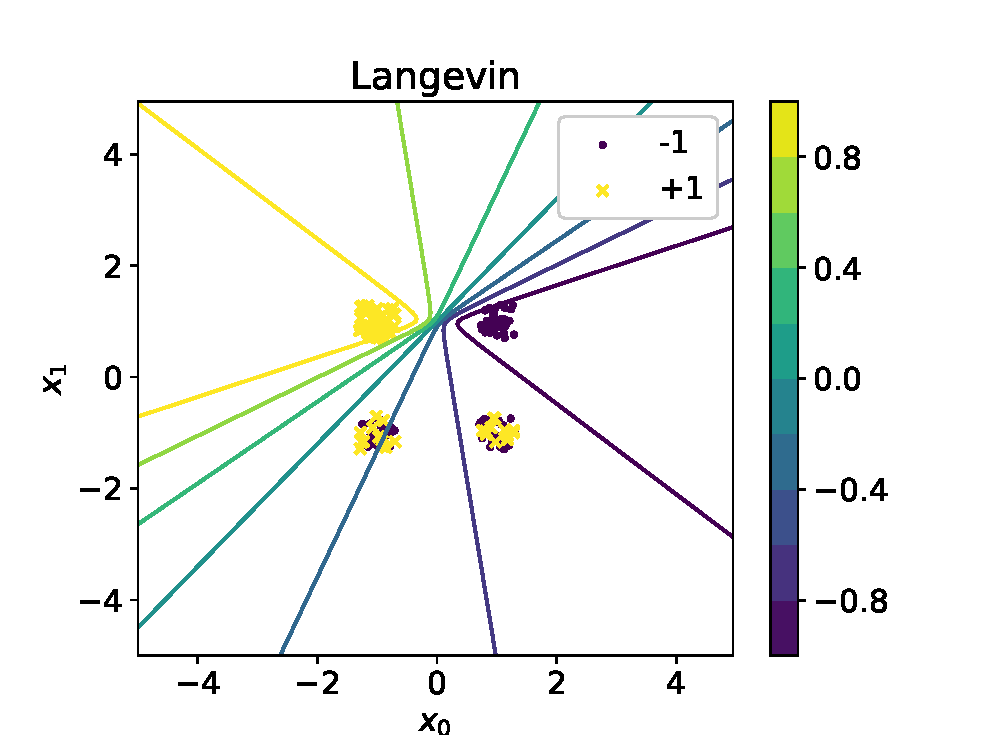
\includegraphics[width = \textwidth]{figures/chapter3/langevin_lh.eps}
    \caption{Separation boundary of Langevin perceptron. The assigned boundaries are broader than for the quantum perceptron. Also, the two noisy classes get different expectation values assigned to them even though they are equally noisy. In the quantum perceptron these samples are assigned an equal probability, so the uncertainty in the data is captured correctly.}
    \label{fig:langevin_lh}
\end{figure}

\noindent Even though we get a similar model separation boundary as for the quantum perceptron, the magnetization perceptron loses some of the elegance of the quantum description. The qubit is an inherently binary system, with states that can be measured and directly correspond to the class labels. For the magnetization perceptron we have to choose the $xz$-plane as the threshold for classification. The $\sigma^x$ operator provides a very natural way of considering flipped labels in the quantum perceptron. Also, the extension to qudits is very natural if we consider the $\text{SU}(C)$ representations for $C$ classes. For a paramagnetic material this is less obvious, since we would have to extend physical space to $1 + C$ dimensions. 

\section{Entangled Qubit Regression} \label{sec:qubit_ent}

As another followup of the critique that the model is not quantum we ask the question: can we utilize quantum effects besides the superposition principle? The answer turns out to be yes. With a simple extension we can build a machine learning model from an entangled state. To start, we remember that a general pure state can be written as (see Appendix \ref{sec:density_matrix})
\begin{equation*}
    \ket{\psi} = \frac{1}{Z}\sum_{i,j} h_{ij} \ket{\psi_i}\otimes\ket{\psi_j},
\end{equation*}
where $h_{ij}\in \mathbb{C}$ and $\{\ket{\psi_{i,j}}\}$ form an orthonormal basis for the subspaces $\mathcal{H}_A$, $\mathcal{H}_B$ respectively. The subspaces have dimension 2 for qubits so $i,j \in \{0,1\}$. We must normalize $\ket{\psi}$ accordingly, so $Z= \sqrt{\braket{\psi}{\psi}}=\sqrt{ \sum_{ij} h_{ij}^*h_{ij}}$. This state can be entangled (see Appendix \ref{sec:entanglement}) and we can describe it with a density matrix,
\begin{align*}
    \rho_\mathbf{x} &= \ketbra{\psi}{\psi}\\
    &= \sum_{i,j,i^\prime, j^\prime} h_{ij}^*h_{i^\prime j^\prime} \ket{\psi_i} \otimes \ket{\psi_j}\bra{\psi_{i^\prime}}\otimes\bra{\psi_{j^\prime}}.
\end{align*}
This matrix is of course rank one since we are dealing with a pure state. If we look at the reduced density matrix $\rho_B$ we end up with a mixed state,
\begin{align*}
    \rho_B &= \Tr_A\left\{\sum_{i,j,i^\prime, j^\prime} h_{ij}^*h_{i^\prime j^\prime} \ket{\psi_i} \otimes \ket{\psi_j}\bra{\psi_{i^\prime}}\otimes\bra{\psi_{j^\prime}}\right\}\\
    \rho_B &= \sum_{i,j,i^\prime, j^\prime} h_{ij}^*h_{i^\prime j^\prime}\underbrace{\Tr_A\left\{ \ket{\psi_i}\bra{\psi_{i^\prime}}\right\}}_{\delta_{i, i^\prime}} \otimes \left(\ket{\psi_j}\bra{\psi_{j^\prime}}\right)\\
    \rho_B &= \sum_{i,j, j^\prime} h_{ij}^*h_{i j^\prime}\ket{\psi_j}\bra{\psi_{j^\prime}}.
\end{align*}
If we take $h_{ij} = \vecwk{ij}\cdot\mathbf{x}$ with $\vecwk{ij} \in \mathbb{C}$, then we have an entangled state parametrized by the data. In matrix form the reduced density matrix is given by
\begin{equation*}
    \rho_B = \frac{1}{\sum_{ij} (h_{ij}^2)}\begin{pmatrix}
    h_{00}^2 + h_{10}^2 & h_{00}^*h_{01} + h_{10}^*h_{11}\\
    h_{00}^*h_{01} + h_{10}^*h_{11} &  h_{01}^2 + h_{11}^2
    \end{pmatrix}.
\end{equation*}
As before, we represent the data as a density matrix $\eta_\mathbf{x} = \sqrt{q(y|x)q(y^\prime|\mathbf{x})}$ and minimize the quantum log-likelihood in equation \ref{eq:q_like},
\begin{equation*}
    NLL = -\sum_{\mathbf{x}} q(\mathbf{x}) \Tr{\eta_x\log{\rho_B}}.
\end{equation*}
To update the parameters we will use the numerical gradient $f^\prime(x) = (f(x + \epsilon) - f(x)) / \epsilon$ for all weights $\vecwk{ij}$ of the density matrix. The matrix logarithm of $\rho_B$ can be calculated by diagonalizing $\rho_B$,
\begin{align*}
    \log(\rho_B) = \log(U D U^{\dagger}) = U\log(D) U^{\dagger}.
\end{align*}
Here, $\log(D)$ is a matrix with the logarithm of the eigenvalues on the diagonal, since $\rho_B$ is positive semidefinite these eigenvalues will always be greater than zero and so the logarithm will be well defined. With this model, we can learn nonlinear problems, such as the XOR problem as seen in figure in \ref{fig:entangled_XOR}
\begin{figure}[ht!]
\centering
    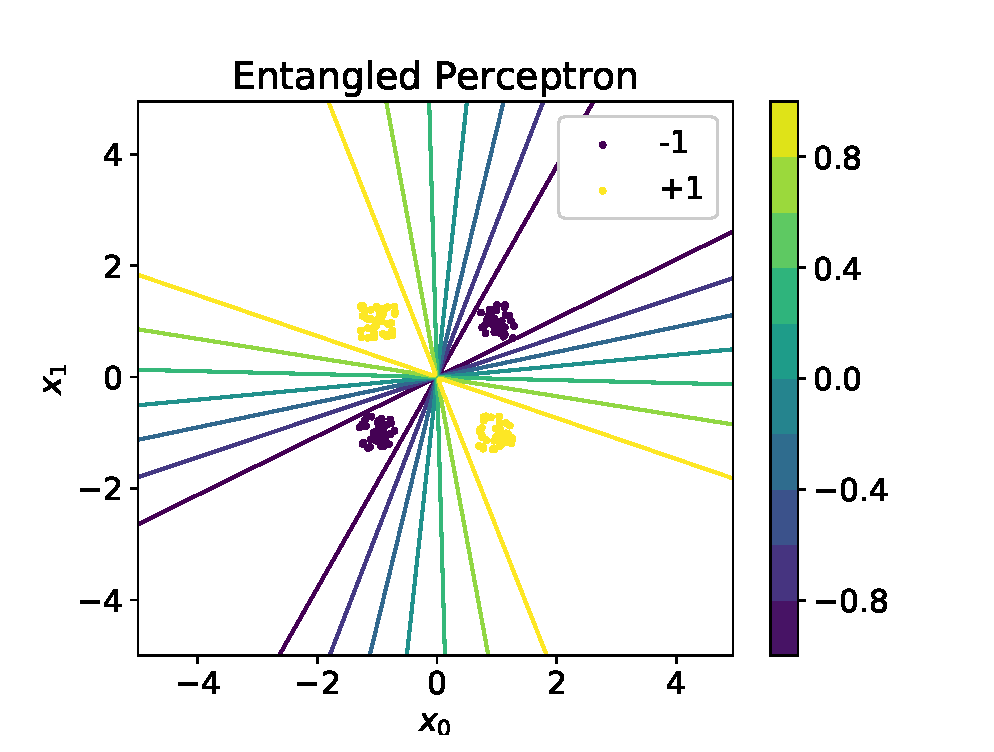
\includegraphics[width=1\linewidth]{figures/chapter3/entangled.eps}
    \caption{The XOR problem solved by two entangled qubits. The hyperbolic separation boundaries allow for the classification of a nonlinear problem.}
    \label{fig:entangled_XOR}
\end{figure}

\noindent Again, let us try to find an analytic expression for the probability boundaries of this model. The reduced density matrix is dependent on four parameters. To study the probability boundaries we study the eigenvectors of the system. First, redefine the density matrix in terms of parameters $a,b,c$,
\begin{align}
    \rho_B = \frac{1}{a+b}\begin{pmatrix}
    a & c\\
    c & b\end{pmatrix} \label{eq:rho_abc},
\end{align}
which we can identify with the previously found single qubit density matrix,
\begin{equation*}
        \rho_\mathbf{x} = \frac{1}{2}\begin{pmatrix}
           1 + m^z  & m^x - im^y\\
           m^x + im^y      & 1 - m^z          
        \end{pmatrix},
\end{equation*}
to find, 
\begin{align*}
    \frac{2a}{a+b} -1 &= m^z\\
    \text{Re}(\frac{c}{a+b}) &= \frac{1}{2}\frac{c + c^*}{a+b} = m^x\\
    \text{Im}(\frac{c}{a+b}) &= \frac{1}{2i}\frac{c - c^*}{a+b} = m^y.
\end{align*}
This allows us to reuse the analysis in sections \ref{sec:probs}. With the use of the eigenvectors we get again that $p(y) = \frac{1}{2}(1 + y\frac{m^z}{\Tilde{m}})$. Setting $p(y=1|\mathbf{x};\mathbf{w}) = p(y=-1|\mathbf{x};\mathbf{w})$ we find
\begin{align}
    \frac{1}{2}(1 + \frac{m^z}{\Tilde{m}}) &= \frac{1}{2}(1 - \frac{m^z}{\Tilde{m}})\nonumber\\
    \frac{m^z}{\Tilde{m}} &= 0,
\end{align}
which is solved for $m^z=0$. But unlike before the trivial solution $m^z=0$ requires us to solve an additional equation,
\begin{align}
    \frac{2a}{a+b} -1 = 0\nonumber\\
    a - b = 0\nonumber\\
    h_{00}^2 + h_{10}^2 - h_{01}^2 - h_{11}^2 = 0 \label{eq:boundary_ent}.
\end{align}
Before we continue, we need to introduce the concept of quadratic forms. The square of a dot product can be written as
\begin{align*}
    h_{ij} h_{kl} &= (\mathbf{w}_{ij} \cdot \mathbf{x}) (\mathbf{w}_{kl} \cdot \mathbf{x}) =\sum_{\mu, \nu} w_{ij}^\mu x^\mu w_{kl}^\nu x^\nu = \mathbf{x}^TA_{ijkl}\mathbf{x} = 0.
\end{align*}
If $A$ is symmetric, then $\mathbf{x}^TA\mathbf{x}$ is a quadratic form. However, the form $ \mathbf{x}^TA_{ijkl}\mathbf{x}$, is not symmetric since in general ${w}_{ij}^\mu \neq {w}_{kl}^\nu$. We can redefine ${w}^{sym}_{ijkl} = \frac{1}{2}({w}^{0}_{ij}{w}^{1}_{kl} + {w}^{1}_{ij}{w}^{0}_{kl})$, ${w}^{00}_{ijkl} = {w}_{ij}^0 {w}_{kl}^0$ and ${w}^{11}_{ijkl} = {w}_{ij}^1 {w}_{kl}^1$ so that we can define a matrix $B$ that is symmetric in terms of the weights $ {w}^{sym}_{ijkl}$, ${w}^{00}_{ijkl}$ and $ {w}^{11}_{ijkl}$ so that $ \mathbf{x}^TB_{ijkl}\mathbf{x}$ is a quadratic form. We can use the fact that a quadratic form describes a quadric surface, e.g., surfaces that are described by the equation
\begin{equation}
    \mathbf{x}^T Q_{ij} \mathbf{x} + \mathbf{R} \mathbf{x} + \mathbf{P} = 0.
    \label{eq:quadric_equation}
\end{equation}
Let us consider the two-dimensional projection of some high-dimensional manifold. The quadric surface (setting $x_1=x$ and $x_2=y$ for the moment) is given by
\begin{equation}
    a x^2 + 2bxy + cy^2+ 2dx +2fy +g = 0,
    \label{eq:quadric_params}
\end{equation}
where $a=w^{00}_{ijkl}$, $b ={w}^{sym}_{ijkl}$, $c=w^{11}_{ijkl}$ and $d=f=g=0$. If we would add a bias, with $x_3=1$, then $d$, $f$ and $g$ would be nonzero. The different types of curves that we get for different values of these parameters are called conic sections, since they are created by the intersection of a plane with a cone. See figure \ref{fig:conic_sections}. The coefficient $b$ can always be set to zero by rotation of the coordinate system \cite{Weisstein}. Equation \ref{eq:boundary_ent} is a linear combination of quadratic forms, which is clearly also a quadratic form.
\begin{figure}
    \centering
    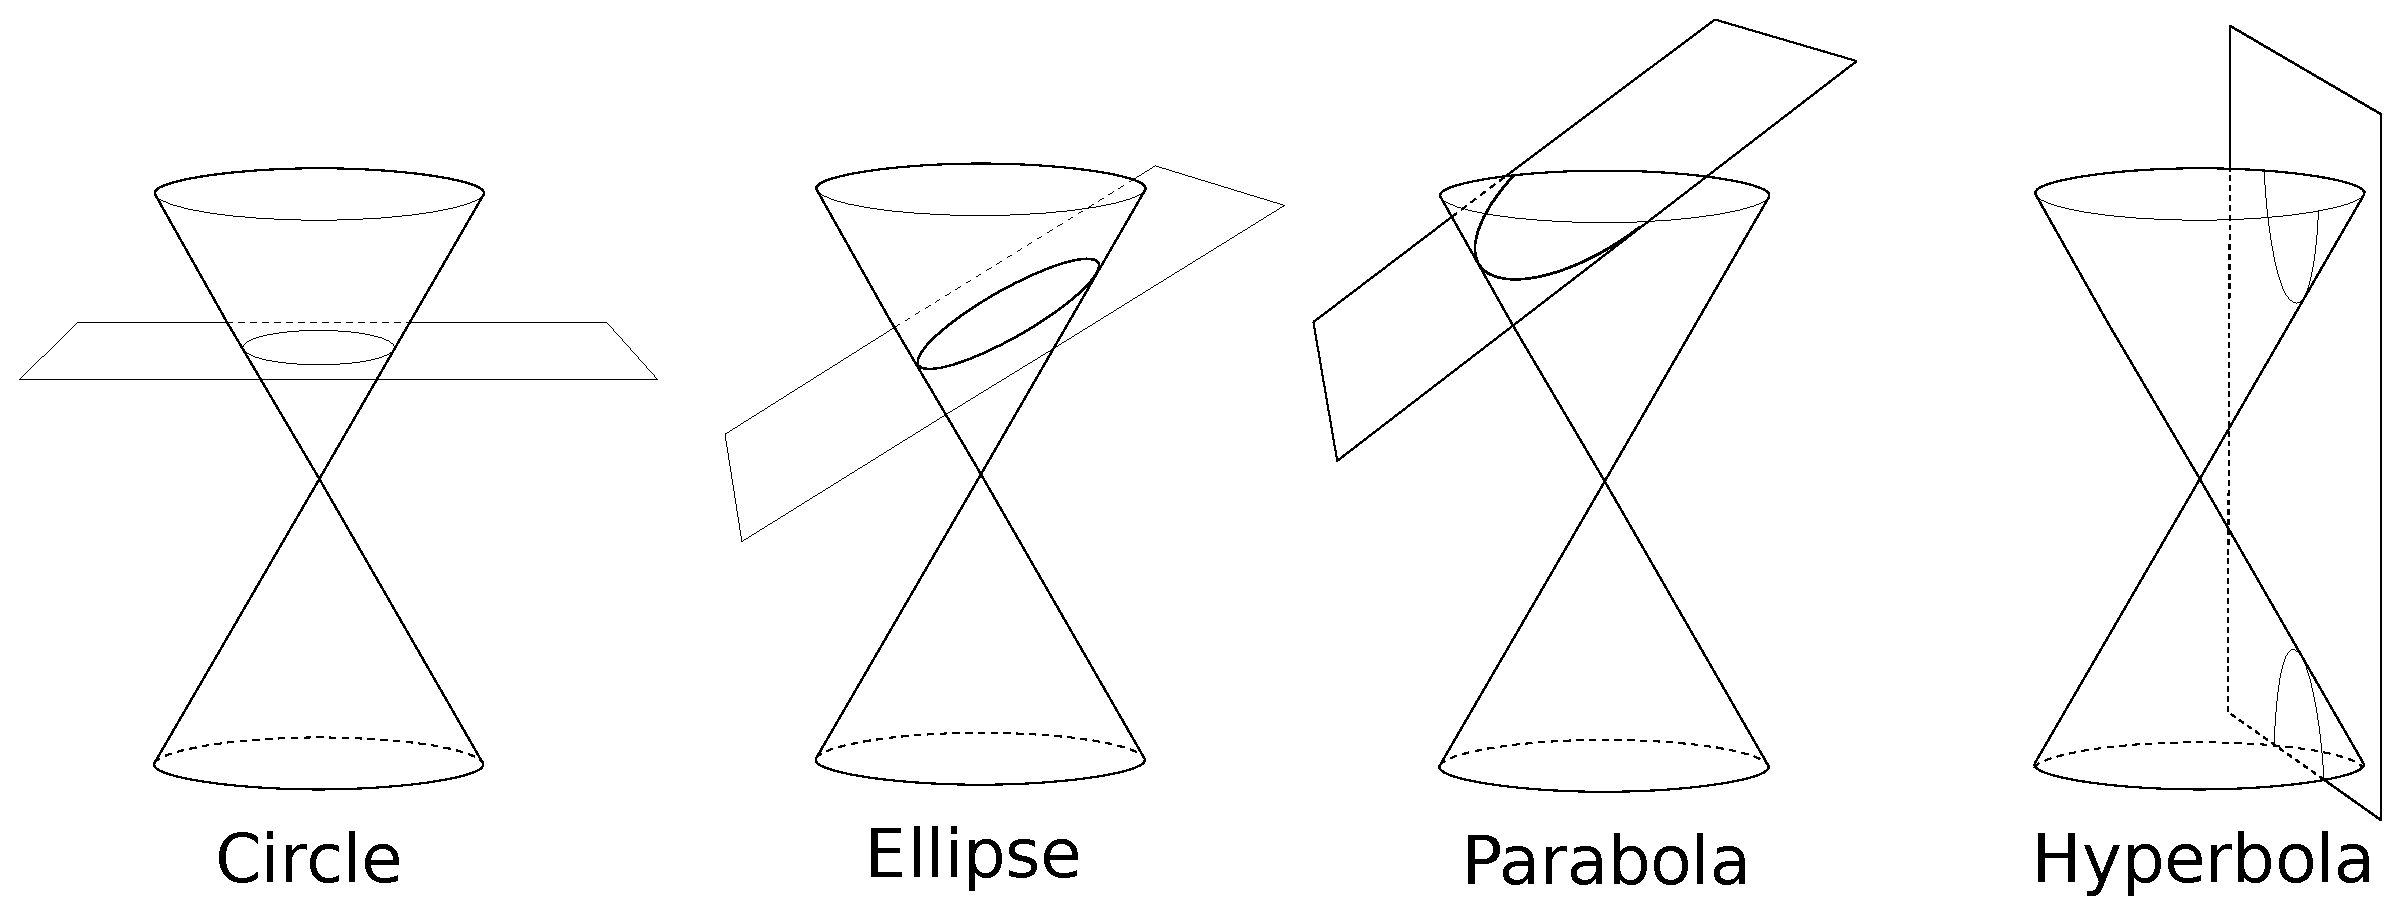
\includegraphics[width=\textwidth]{figures/chapter3/conic_sections.eps}
    \caption{4 of the non-degenerate (real) conic sections. We can also have a single point, if we take a plane at the apex of the cones, or a line the plane is tangent to the surface of the cone.}
    \label{fig:conic_sections}
\end{figure}
The classification of which conic section we obtain is dependent on the following quantities \cite{Zwillinger2002}:
\begin{align*}
    \Delta = \det
    \begin{pmatrix}
    a & b & d \\
    b & c & f\\
    d & f & g
    \end{pmatrix}, \;
    J = \det
    \begin{pmatrix}
    a & b \\
    b & c 
    \end{pmatrix}, \;
    K = \det
    \begin{pmatrix}
    a & d \\
    d & g 
    \end{pmatrix} + \det
    \begin{pmatrix}
    c & f \\
    f & g 
    \end{pmatrix},\; I = a + b
\end{align*}
Based on these we can determine the different geometric shapes of the quadric as can be seen in table \ref{tab:conics}.
\begin{table}[ht!]
    \centering
    \caption{Since we only have real weights, we can only have real conics, so the shapes with a star are excluded.}
    \begin{tabular}{|c | c | c| c |l|}
         \hline $\Delta$ & J & $\Delta / I$ & K & Conic Type\\\hline
         $\neq 0$ & $<0$ & & & Hyperbola \\
         $\neq 0$ & $0$ & & & Parabola\\
         $\neq 0$ & $>0$ & $<0$ & &  Ellipse\\
         $\neq 0$ & $>0$ &  $>0$ & & Imaginary ellipse *\\
         $0$ & $<0$ & & & Intersecting lines\\
         $0$ & $>0$ & & &  Point\\
         $0$ & $0$ & & $<0$ & Distinct Parallel lines \\
         $0$ & $0$ & & $>0$ & Imaginary parallel lines *\\
         $0$ & $0$ & & $0$ & Coincident lines \\\hline
    \end{tabular}
    \label{tab:conics}
\end{table}

\noindent What can we say about the probability curves $p(y=1|\mathbf{x};\mathbf{w}) = \frac{1}{2}(1+\epsilon)$? We have
\begin{align}
    \frac{m^z}{\Tilde{m}} &= \epsilon \nonumber\\
    m^z & = \epsilon \Tilde{m},
    \label{eq:prob_curve_abc}
\end{align}
which looks complicated, because calculating  $\Tilde{m} = \sqrt{\sum_k (m^k)^2}$ with the previously made identifications between $a,b,c$ and $m^x, m^y, m^z$ looks cumbersome. We remember that $\Tilde{m}$ also shows up in the eigenvalues of the density matrix as $\lambda_\pm = \frac{1}{2}(1 \pm \Tilde{m})$ in equation \ref{eq:eigenvalue}. If the eigenvalues of equation \ref{eq:rho_abc} admit a similar form, we might be able to find a simple form for $\Tilde{m}$. The matrix in equation \ref{eq:rho_abc} has characteristic polynomial $(a-\lambda)(b-\lambda)-c^2 = \lambda^2 - \lambda(a+b) + ab - c^2$. Solving this equation and taking the factor in front into account gives $\lambda_{\pm}^\prime = \frac{1}{2}(1 \pm \sqrt{(a-b)^2 +4c^2} / (a+b)$. We can identify $\Tilde{m} = \sqrt{(a-b)^2 +4c^2} / (a+b)$. Substituting these identifications in equation \ref{eq:prob_curve_abc} gives
\begin{align*}
    \frac{2a}{a+b} -1 &= \epsilon\frac{\sqrt{(a-b)^2 +4c^2}}{(a+b)}\\
    a-b &= \epsilon \sqrt{(a-b)^2 +4c^2}\\
    a^2 - b^2 - 2ab&= \epsilon^2 (a^2 + b^2 - 2ab +4c^2)\\
    (a - b )^2 (1-\epsilon^2) - \epsilon^2 4c^2 &= 0,
\end{align*}
which gives back the original condition $a-b=0$ in the case that $\epsilon=0$,
\begin{align*}
    (a - b ) \sqrt{1-\epsilon^2} &= \pm\epsilon 2c \\
    (a - b )  &= \pm\frac{\epsilon}{\sqrt{1-\epsilon^2}} 2c.
\end{align*}
Since this is again a linear combination of quadrics, we expect the separation boundaries to be quadric as well. We can observe some different quadratic separation boundaries in figure \ref{fig:3_problems}.

\begin{figure*}[htb!]
        \centering
        \subfloat[]{
          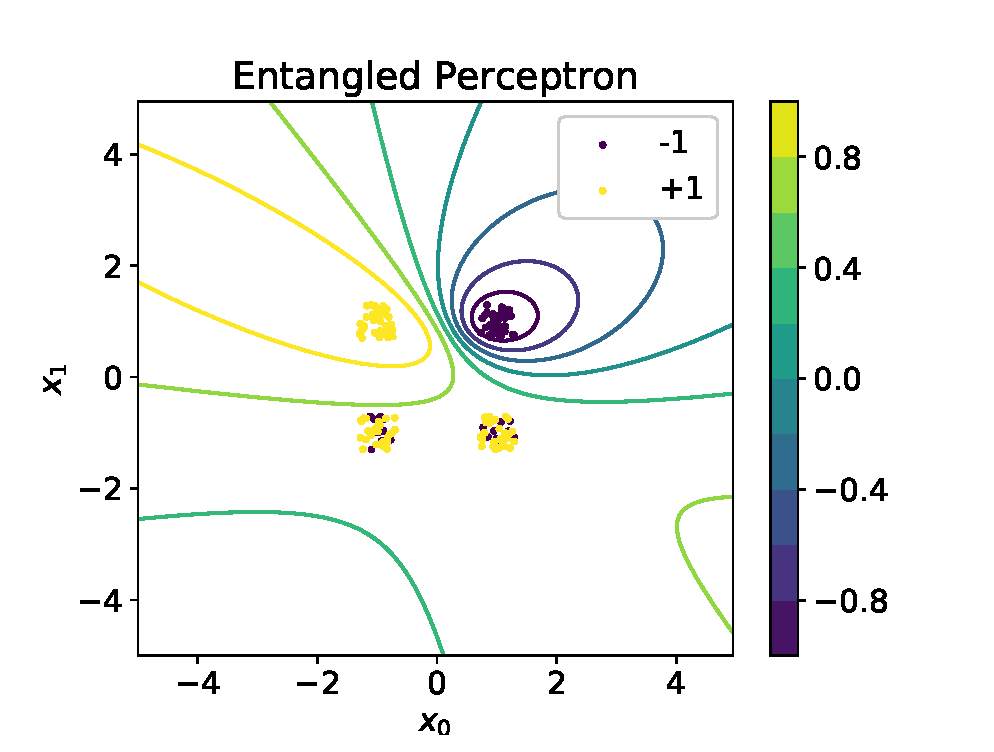
\includegraphics[width=0.5\textwidth]{figures/chapter3/grid_0.eps}
        }
        \subfloat[]{
          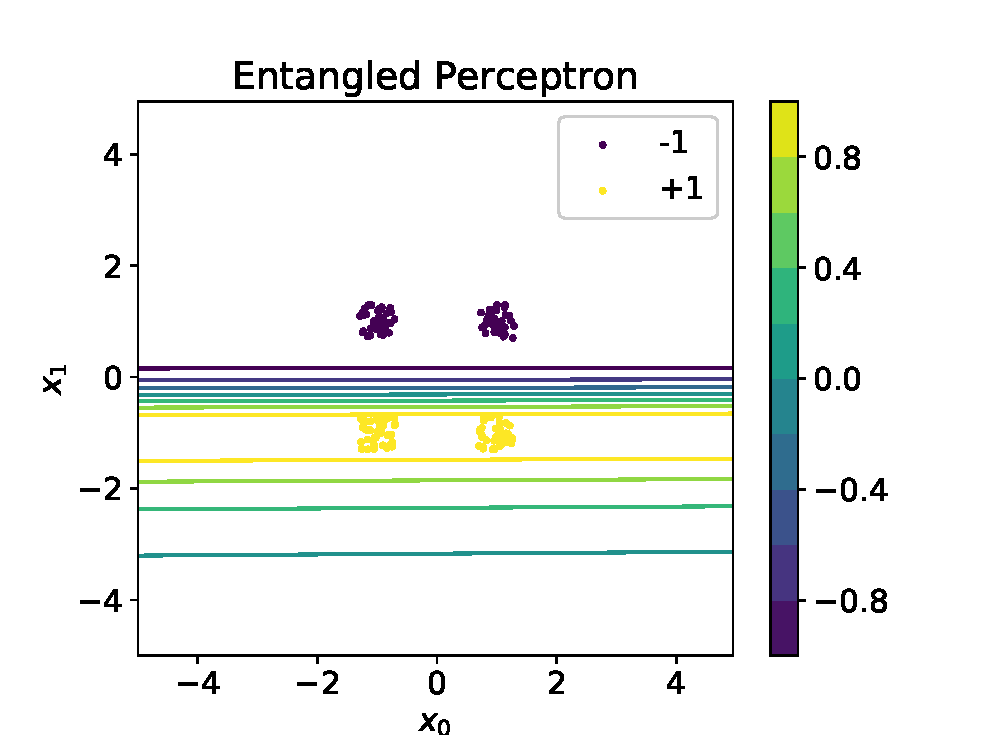
\includegraphics[width=0.5\textwidth]{figures/chapter3/grid_1.eps}
        }\newline
        
        \subfloat[]{
          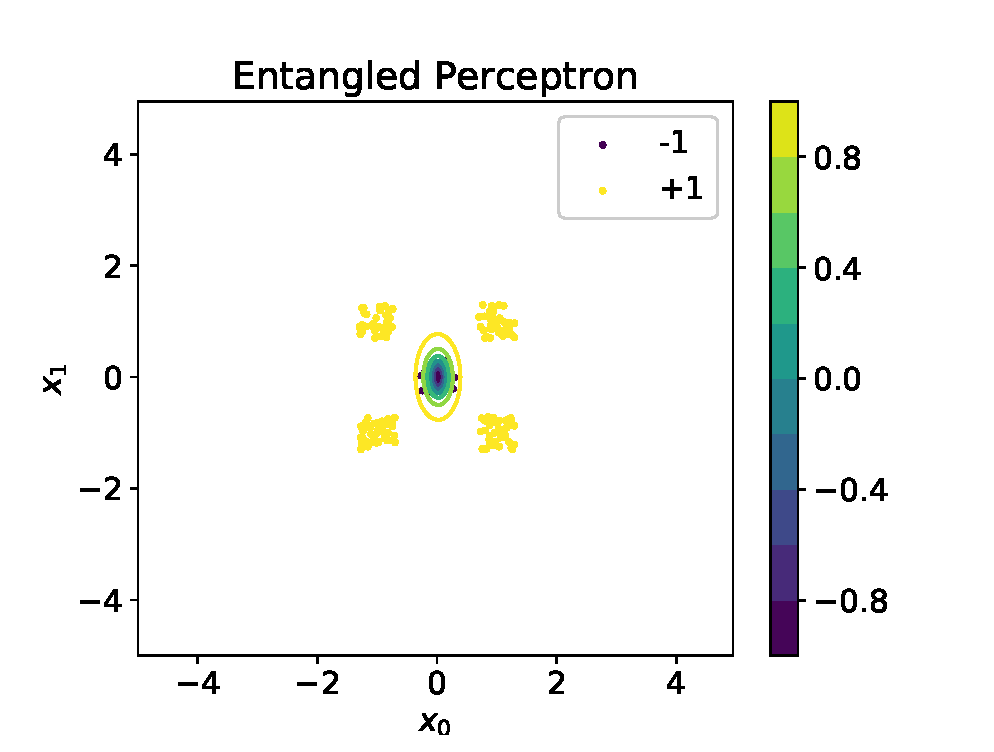
\includegraphics[width=0.5\textwidth]{figures/chapter3/grid_2.eps}
        }
        \subfloat[]{
          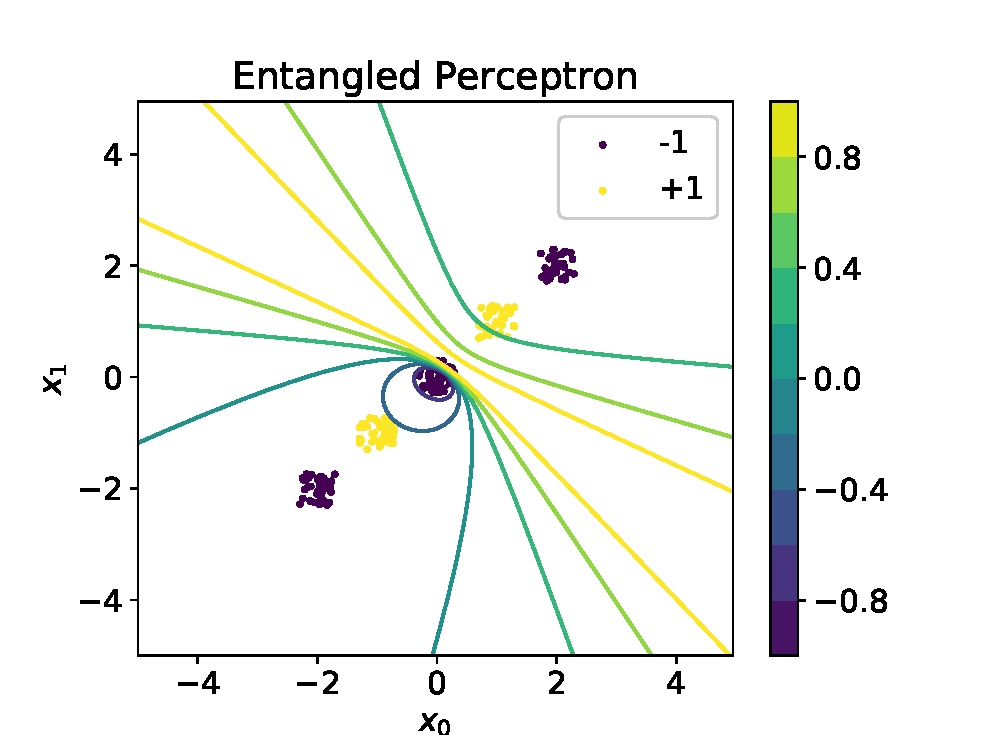
\includegraphics[width=0.5\textwidth]{figures/chapter3/grid_3.eps}
        }
        \caption{Separation boundaries of the entangled perceptron for additional two-dimensional problems. \textbf{(a)} We can still learn the same noisy problem that we studied in section \ref{sec:results}, only now with quadric surfaces. \textbf{(b)} A quadric surface can also consist of parallel lines, allowing us to learn linearly separable problems. \textbf{(c)} For this specific problem we can find an elliptical separation boundary to perfectly classify the data. \textbf{(d)} Problems that cannot be solved with a quadric surface are still problematic and lead to bad solutions.} 
        \label{fig:3_problems}
    \end{figure*}
    
\clearpage
\noindent It is clear that the method of entangling qubits can also be used for multiple classes and continuous classes. See figures \ref{fig:entangled_qutrit} and \ref{fig:entangled_qutrit_cont}. 

\begin{figure}[htb!]
    \centering
    \makebox[\textwidth][c]{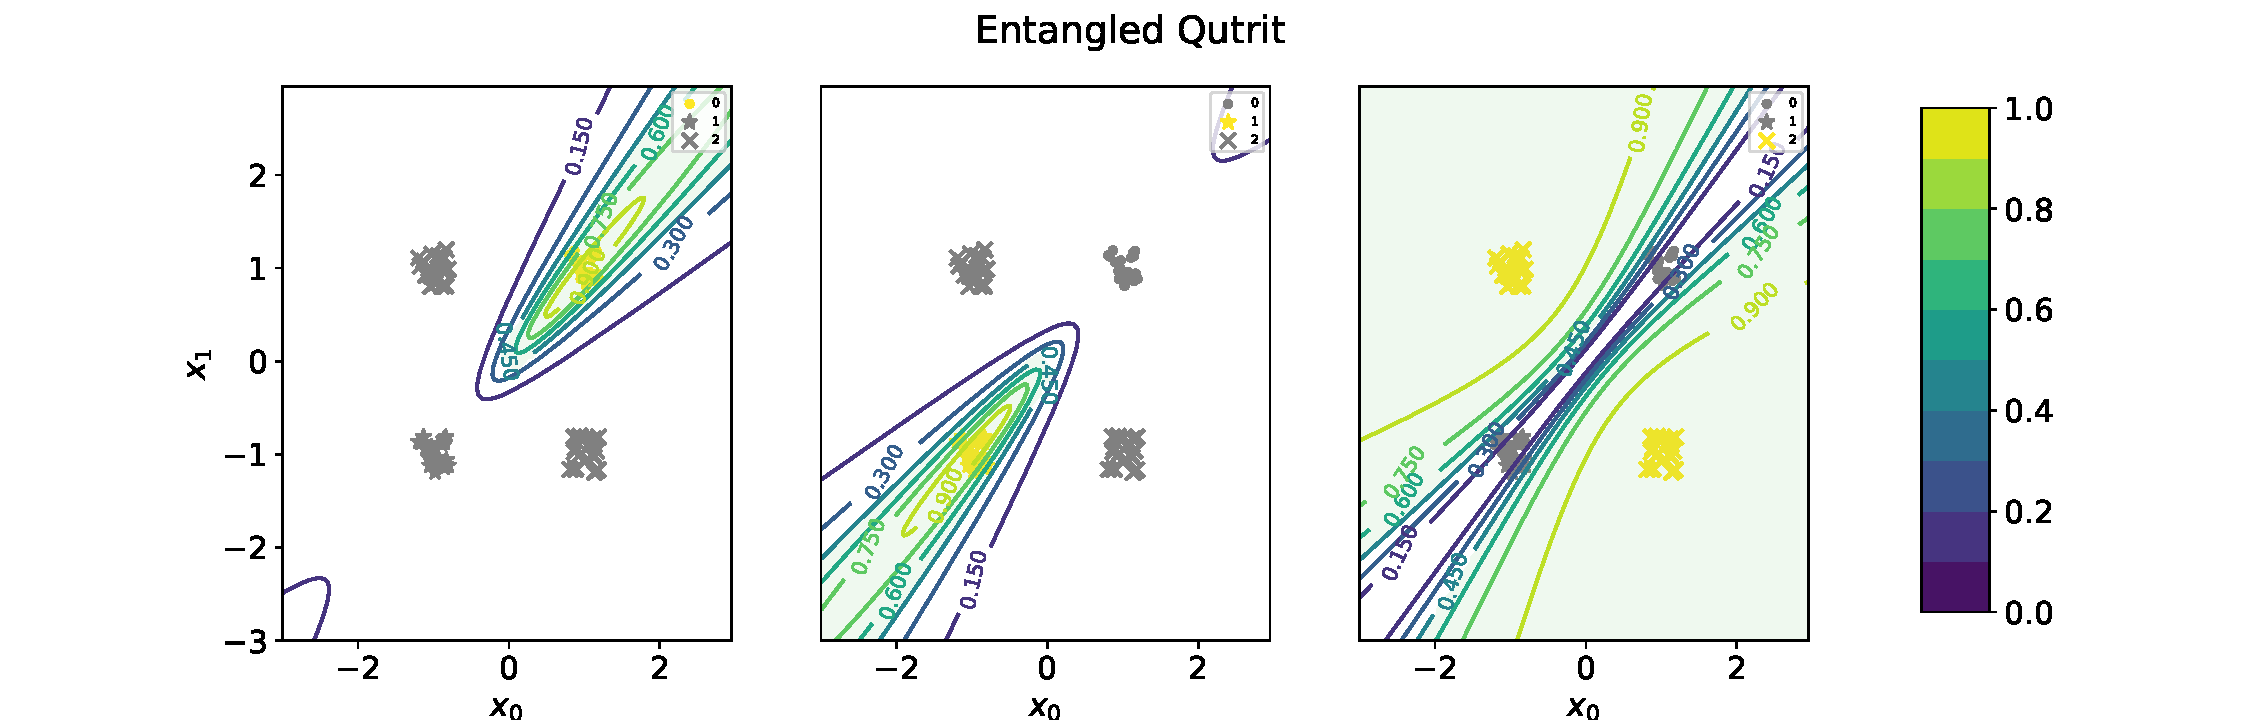
\includegraphics[width = 1.4\textwidth]{figures/chapter3/entangled_qutrit.pdf}}
    \caption{Separation boundary of entangled qutrit. For non-noisy nonlinear data we obtain perfect classification.}
    \label{fig:entangled_qutrit}
\end{figure}

\begin{figure}[htb!]
    \centering
    \makebox[\textwidth][c]{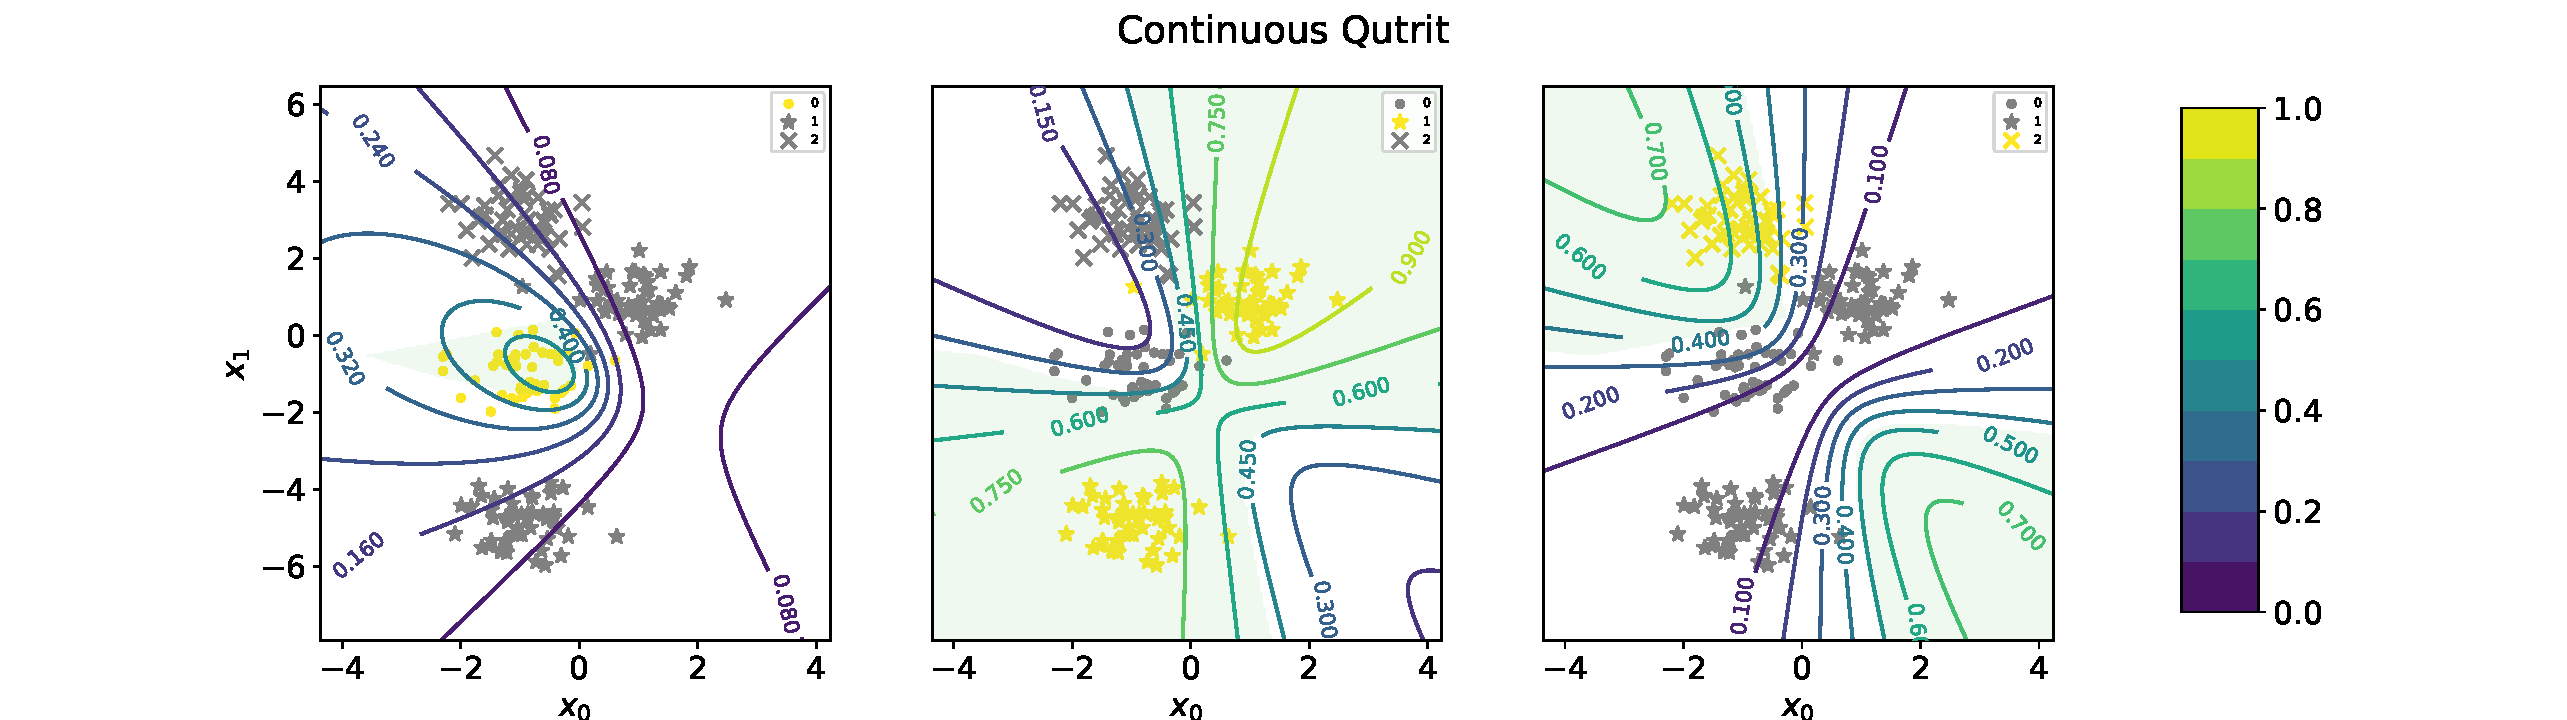
\includegraphics[width = 1.4\textwidth]{figures/chapter3/cont_qutrit_entan.pdf}}
    \caption{Separation boundary of entangled qutrit with continuous data. A combination of elliptic and hyperbolic separation boundaries makes it possible to learn this continuous data set.}
    \label{fig:entangled_qutrit_cont}
\end{figure}

\noindent Entangling more than 2 qubits with this method might seem worthwhile. However, this will not give any additional features. The wave function for multiple qubits is given by
\begin{equation*}
    \ket{\psi} = \frac{1}{Z}\sum_{i_1,\ldots i_n}  h_{i_1,\ldots i_n}\ket{\psi_{i_1}}\otimes \ldots \otimes h_{i_n}\ket{\psi_{i_n}},
\end{equation*}
which contains fields $h_{ij}$ corresponding to the basis state $\ket{\psi_{i_1}}\otimes \ldots \otimes h_{i_n}\ket{\psi_{i_n}}$. When we trace out a part of the system to create a reduced density matrix, we always end up with a linear combination of quadratic terms $h_{ij}^2$. The number of terms in this linear combination scales with the dimension of the total Hilbert space. But since all these terms are at most quadratic, the boundaries are always a quadric surface, since a linear combination of quadric surfaces is still a quadric surface, as noted before. Entangling more qubits thus only increases the number of parameters that determine the shape of the quadric surface.\newline

\noindent To summarize, the quantum perceptron can be extended to learn nonlinear boundaries, such as the XOR problem. We have shown that this is possible because the entangled perceptron can learn quadric surfaces due to the quadratic parametrization of the reduced density matrix. This extension can be combined with the previous results to learn multiclass continuous data. We retain the robustness with respect to noise, because we still minimize the quantum log-likelihood with respect to a density matrix with off-diagonal elements.


\section{Physical System}

Up to this point we have taken a lot of freedom with the description of the model $\rho_\mathbf{x}$. We have parametrized density matrices and wave functions in the most general way possible by choosing the system Hamiltonian to be
\begin{equation*}
    H = \sum_k h^k \sigma^k.
\end{equation*}
While this description is convenient, it does not take the physical constraints of a system into account. As it turns out, we can still learn non-trivial problems if we limit the degrees of freedom significantly. Consider the Hamiltonian of two coupled qubits, both with transverse fields $h_1$ and $h_2$,
\begin{equation*}
    H_1 = h_{1} {\sx}_1 + h_{2} {\sx}_2 + J_{12} {\sz}_1 {\sz}_2,
\end{equation*}
with corresponding density matrix $1/Z e^{\beta H}$. The subindex of the Pauli matrix indicates the spin location. We are interested in this system, because it can be realized easily experimentally. By tuning the transverse fields we can control entanglement, which would be an interesting way to implement the perceptron. In order to minimize the quantum likelihood in equation \ref{eq:q_like} we have to obtain a single qubit density matrix, since $\eta_\mathbf{x}$ is a single qubit data density matrix. By tracing out one qubit we get $\rho_{red} = \Tr_2\{\rho\}$, which allows us to minimize the quantum log-likelihood,
\begin{equation*}
    \mathcal{L}_{phys} = -\sum_{\mathbf{x}} q(\mathbf{x}) \Tr_1\{\eta_\mathbf{x}\log( \rho_{red})\}.
\end{equation*}
Calculating $\Tr_2\{\rho\}$ is not easy. We either have to diagonalize a $4\times4$ matrix or approximate $\exp{H}$. Both can be done numerically, but we are interested in an analytic expression of the reduced exponent. Finding an analytic expression is cumbersome, since we have to write out 
\begin{equation*}
    e^H = \sum_{i=0}^\infty \frac{H_1^n}{n!},
\end{equation*}
to some order, perform the partial trace over the second subspace and try to extract a nice expression for the sum generating this expression (see Appendix \ref{sec:partial_tr}). However, this might give some insight in the problems that we can learn with this physical system setup. The hope is that calculating the first five orders of H might allow us to write down an infinite series expansion for the partial trace of the exponent. If this retains the infinite radius of convergence of the exponent, we might be able to study the partial trace of an exponential operator in the limit $\beta\to \infty$ in an analytic way. We calculate the first five non-trivial terms,
\begin{equation*}
    \frac{1}{Z}e^H_1 \approx \frac{1}{Z} \left(1 + H_1 + \frac{1}{2}H_1^2 + \frac{1}{6} H_1^3 + \frac{1}{24} H_1^4+ \frac{1}{120} H_1^5\right) + \mathcal{O}(h^6).
\end{equation*}
If we trace over the second qubit we get the reduced density matrix. The full derivation can be found in the Appendix \ref{sec:phys_sys}. The first five orders of $H$ are
\begin{align*}
    H_1 &= h_1 {\sx_1} + h_2 {\sx_2} + J^{z}_{12} {\sz}_1 {\sz}_2,\\
    H_1^2 & = c + 2 h_1 h_2 {\sx_1} {\sx_2},\\
    H_1^3 &= c {H_1} + 2 \left(h_1^2 h_2 {\sx_2} +  h_1h_2^2 {\sx_1} + J_{12}^z h_1 h_2 {\sy_1} {\sy_2}\right),\\
    H_1^4 &= (c^2 + 4 (h_1 h_2)^2 + 4 (h_1 h_2)^2),\\
    H_1^5 &=  c^2 {H_1} + 4c \left(h_1^2 h_2 {\sx_2} +  h_1h_2^2 {\sx_1}\right) + 4 h_1 h_2(h_1^2 h_2 {\sx_1} + h_1 h_2^2 {\sx_2} - J_{12}h_1 h_2{\sz_1}{\sz_2}).
\end{align*}
Calculating the partial trace and taking the factorial coefficients into account then gives
\begin{align}
     \Tr_2\{\rho\}  &\approx   \frac{1}{2}\left(1 + \overbrace{h_1\left(1  - \frac{1}{3} \left[h_1^2 + J_{12}^2 \right]  + \frac{2}{15}\left(\left[h_1^2 + J_{12}^2\right]^2\right)+2h_2^2 J_{12}^2\right)}^{m^x}\sx_1\right) + O(h^6)\label{eq:full_expression}\\
     & = \frac{1}{2}(1 + m^x\sx_1)\nonumber.
\end{align}
Note that in the case that $J_{12}\to0$ we only get back a dependence on parameters of spin 1. This is the expected behaviour, because if there is no interaction the full exponent factorizes and all dependence on $h_2$ should be eliminated by the trace. Our goal is now to find a sum which generates equation \ref{eq:full_expression}. Remember that the hyperbolic tangent is given by
\begin{equation*}
    \tanh(x) = x\left(1 - \frac{x^2}{3} + \frac{2x^4}{15}\right)+ O(h^7).
\end{equation*}
Substituting $x= [h_1^2 + J_{12}^2]^\frac{1}{2}$ gives
\begin{align*}
    \tanh([h_1^2 + J_{12}^2]^\frac{1}{2}) = [h_1^2 + J_{12}^2]^\frac{1}{2}\left(1 - \frac{1}{3}[h_1^2 + J_{12}^2] + \frac{2}{15}[h_1^2 + J_{12}^2]^2\right).
\end{align*}
Multiplying with $\frac{h_1}{[h_1^2 + J_{12}^2]^\frac{1}{2}}$ gives back the original expression, except for the $2h_2^2 J_{12}^2$ term,
\begin{align*}
    \tanh([h_1^2 + J_{12}^2]^\frac{1}{2})\frac{h_1}{[h_1^2 + J_{12}^2]^\frac{1}{2}}= h_1\left(1  - \frac{1}{3} \left[h_1^2 + J_{12}^2 \right]  + \frac{2}{15}\left[h_1^2 + J_{12}^2\right]^2\right) + O(h^7).
\end{align*}
Using a Mathematica script, we were able to determine even more terms. Our hope was that some structure might appear that would allow us to resum the $2h_2^2 J_{12}^2$ in some way. But alas, it seems that the extra terms cannot be resummed easily to a nice algebraic expression with our approach\footnote{Using a different approach \cite{DeZela2014}, Eduardo Dominiquez was able to determine an algebraic expression for the reduced density matrix. However, this method relies on calculating the algebraic expressions of the eigenvalues of a H, which becomes quite involved for more complex Hamiltonians. For our simple system this becomes 
\begin{align*}
    \Tr_2\{\rho\} &= \frac{1}{2}\left(1 + \frac{1}{\cosh{E_1} + \cosh{E_2}}\left(\frac{h_1 + h_2}{E_1}\sinh{E_1} + \frac{h_1 - h_2}{E_2}\sinh{E_2} \right)\sx_1\right),
\end{align*}
with
\begin{align*}
    E_1 &= \sqrt{(h_1+h_2)^2+J_{12}}\\
    E_2 &= \sqrt{(h_1-h_2)^2+J_{12}}.
\end{align*}}.
\noindent Nonetheless, for small our approximation will do fine. The reduced density matrix can be written as 
\begin{equation}
    \Tr_2\{\rho\} \approx \frac{1}{2}\left(1 + \tanh([h_1^2 + J_{12}^2]^\frac{1}{2})\frac{h_1}{[h_1^2 + J_{12}^2]^\frac{1}{2}} \sx_1 \right) = \frac{1}{2}(1 + m^x \sx_1) \label{eq:tanh_tr}.
\end{equation}
If we want to learn a classical distribution, we need to have at least have a $\sigma_z$ field so that we can control the diagonal elements of the density matrix. Luckily we can exchange $x\Leftrightarrow z$ by a simple basis transformation to obtain this,
\begin{equation*}
    H_1^\prime = h_{1} {\sz}_1 + h_2 {\sz}_2 + J_{12} {\sx}_1 {\sx}_2,
\end{equation*}
which gives
\begin{align*}
     \Tr_2\{\rho\}  &\approx  \frac{1}{2}(1 + m^z\sz_1),
\end{align*}
with $m^x=m^z$ with $h_1\Leftrightarrow h_2$ by symmetry. Based on this derivation, we hypothesize that constructing a system with Hamiltonian $H_1^\prime$ where the field $h_1$ is parametrized as $h_1=\mathbf{x}\cdot \mathbf{w}_1$ will allow us to learn data under the constraints of a physical system. In figure \ref{fig:hx_full} we see that this is indeed possible. Adding a field $g_1 \sx_1$ to $H_1^\prime$ also allows us to also learn the off diagonal elements. The derivation that shows this can again be found in Appendix \ref{sec:phys_sys} (with $x\Leftrightarrow z$). Adding noise to the data points gives us the curved probability boundaries as expected, as can be seen in figure \ref{fig:hx_full_noise}. \newline

\noindent In this section we have shown that the quantum perceptron model can still be learned for a physical system. By tuning a single transverse field we can construct a quantum system whose statistics give us the correct class probability. Adding another external field gives us the curved probability from the original quantum perceptron. Further investigation of exact expressions of reduced density matrices might be an fruitful direction of future research. Also, realizing the setup with a physical system experimentally might be interesting. Although for each field we still need to calculate $h_i = \mathbf{x}\cdot \mathbf{w}_i$ on a classical computer, the rest can be realized on an actual spin system. 
\clearpage
\begin{figure}[htb!]
    \centering
    \makebox[\textwidth][c]{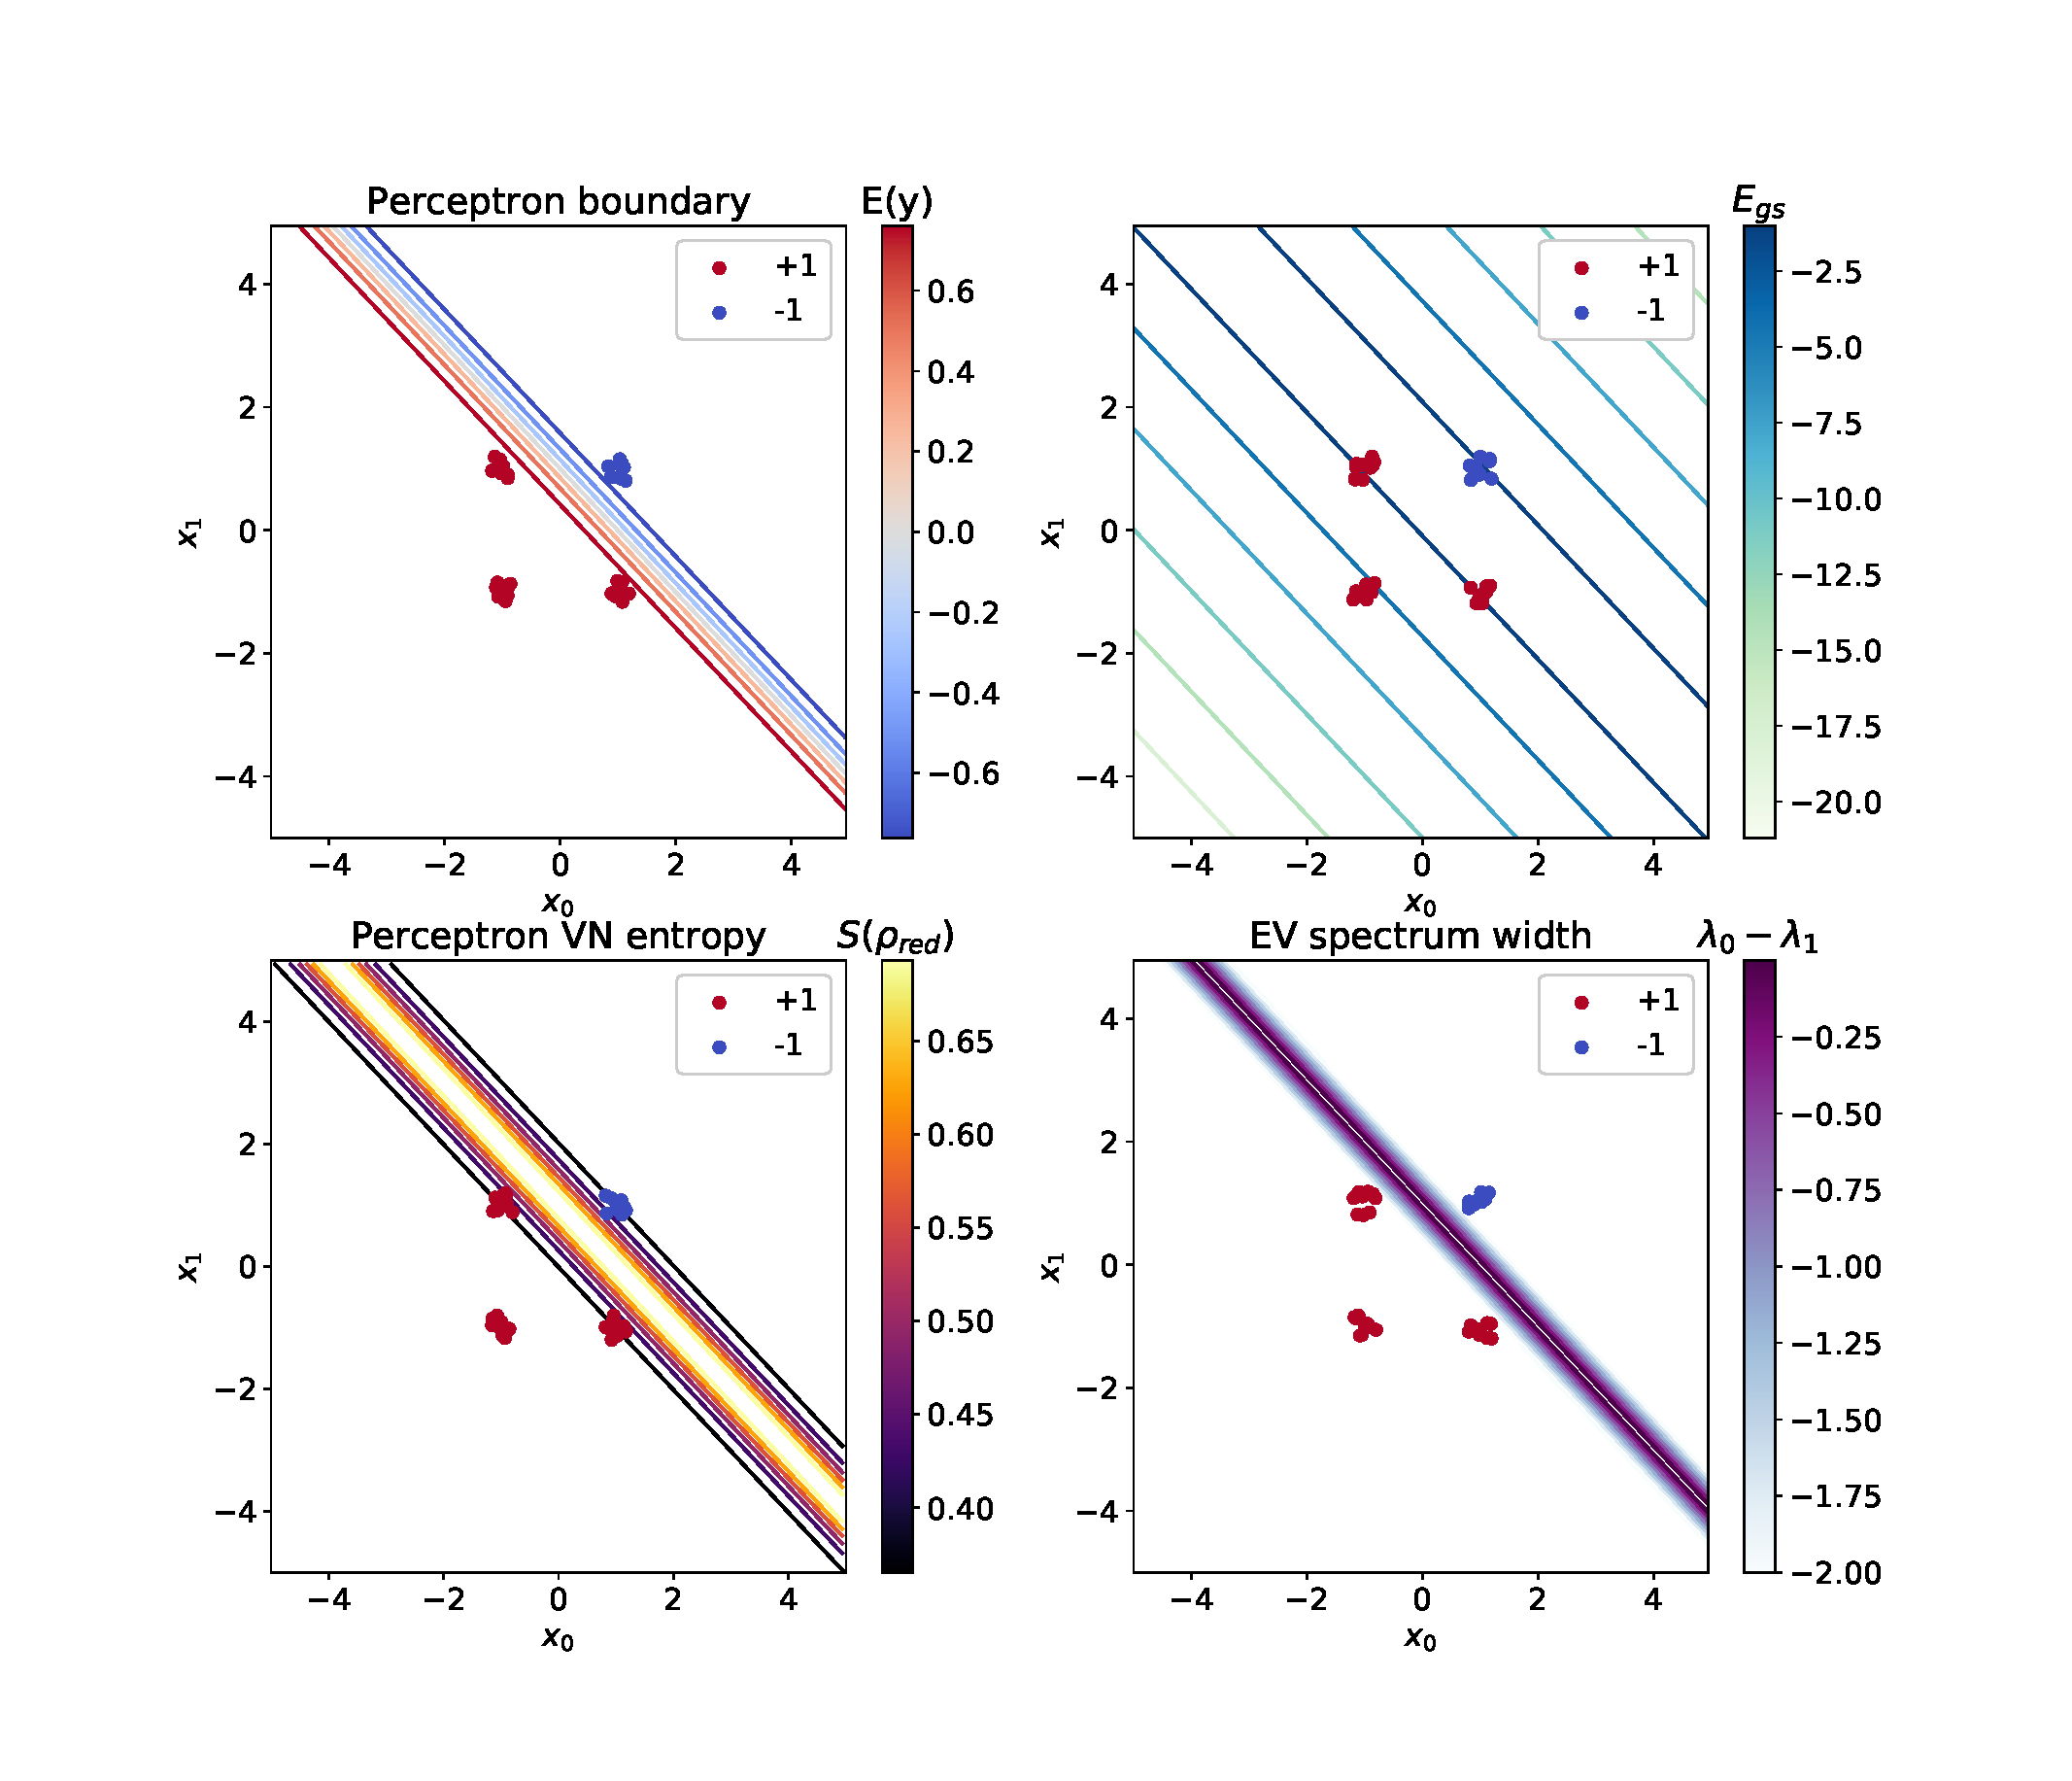
\includegraphics[width=1.1\textwidth]{figures/chapter3/physical_system.eps}}
    \caption{The simple binary classification problem from section \ref{sec:results} learned with a physical quantum system with $J_{12}=1$. To break the degeneracy of the system we add a very small field $0.05\sx$. The probability $p(y|\mathbf{x};\mathbf{w})$ is again constructed by measuring $\expval{\sz_1}$. The top left figure shows the separation boundaries, which are equal to the logistic regression boundaries as expected, but $\expval{\sz_1}$ is limited to the interval $[-0.7,0.7]$. The top right shows us the ground state energy, which is spread symmetrically around the boundary. The bottom left shows the von Neumann entropy (see Appendix \ref{sec:entanglement}). The closer we are to the boundary, the higher the entropy since the state uncertainty increases.In the bottom right we see the how the difference between the energies of the system's state determines the separation boundaries. When the energies are close, there is a large uncertainty about the class label.}
    \label{fig:hx_full}
\end{figure}
\clearpage

\begin{figure}[htb!]
    \centering
    \makebox[\textwidth][c]{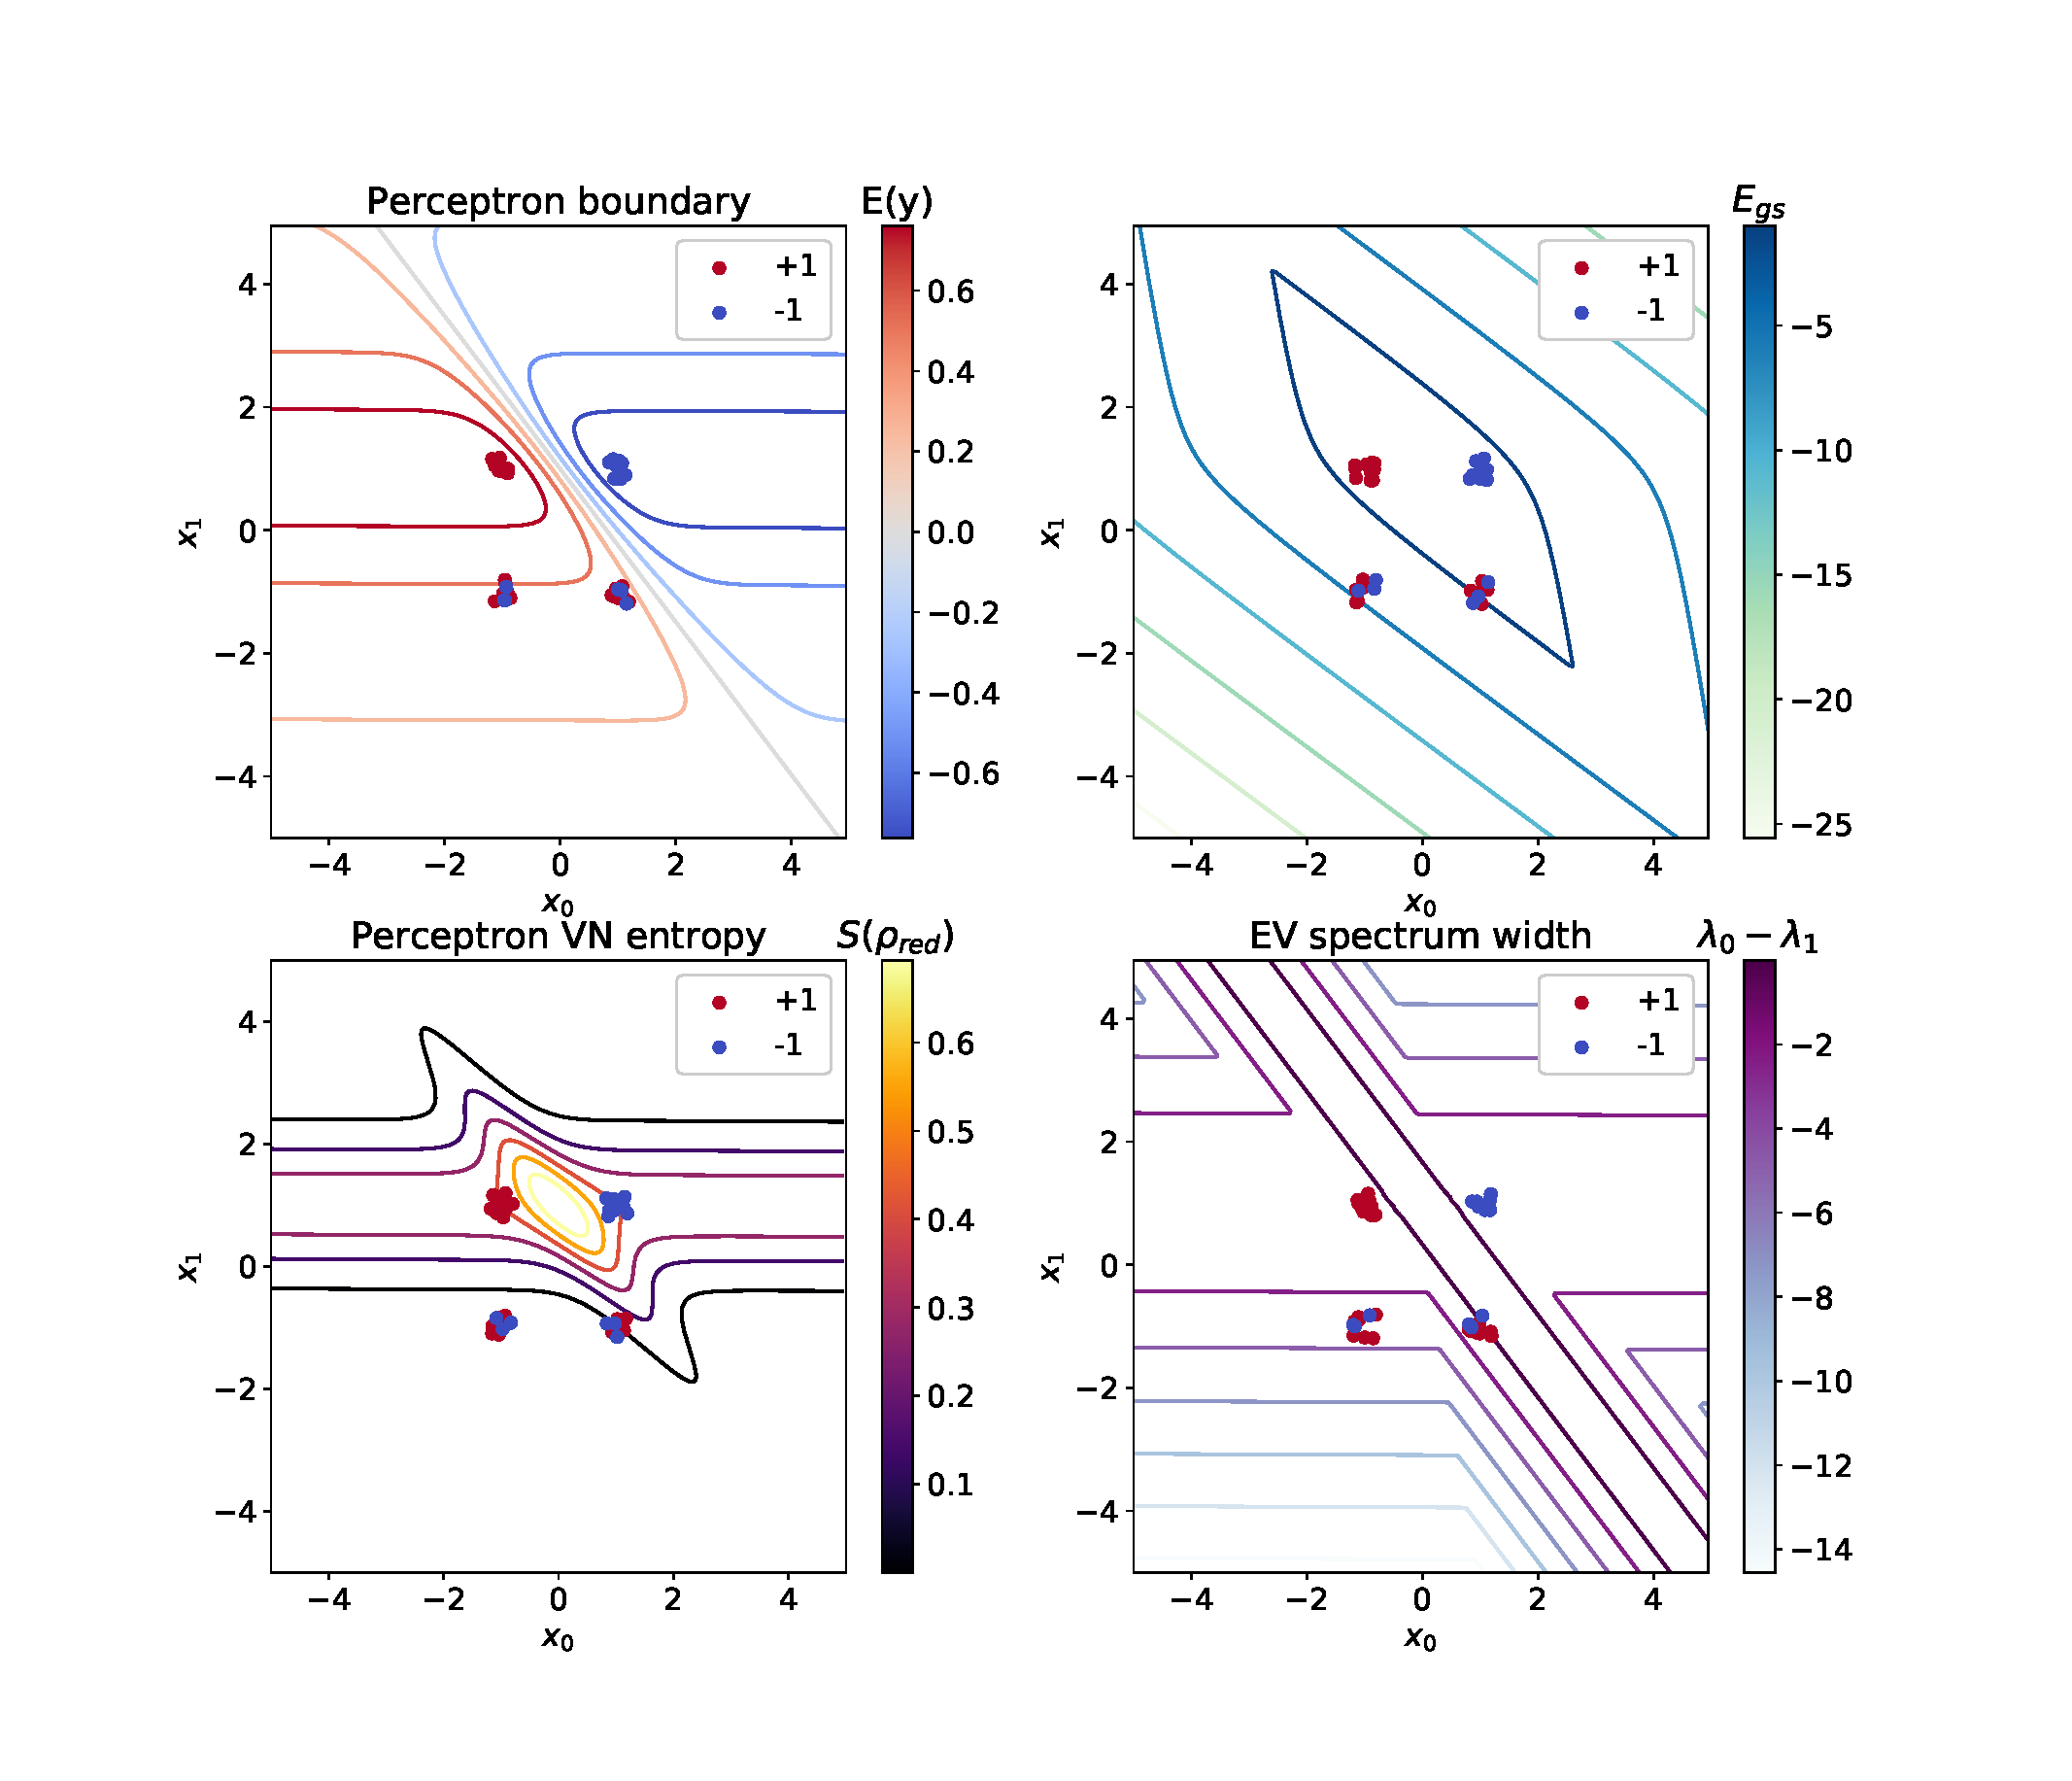
\includegraphics[width=1.2\textwidth]{figures/chapter3/physical_system_noise.eps}}
    \caption{In the top left figure we see that the curved separation boundaries. The probability curves are no longer hyperbolic but look more like flattened parabolas. The maximal von Neumann entropy in the bottom left figure is no longer located on the boundary, but concentrated between the two non-noisy samples to account for the uncertainty about the two noisy samples. The top and bottom right figures reflect the changes in the separation boundary and uncertainty.}
    \label{fig:hx_full_noise}
\end{figure}

\clearpage

\section{ $\Lambda$-operator perceptron}

In Amin's proposal for the quantum boltzmann a density matrix likelihood is constructed by limiting the trace of a modeled density matrix to the diagonal by applying a projection operator $\Lambda(y)$  \cite{Amin2018}. This operator is used to reduce the trace to the visible units of the quantum boltzmann machine. We can use this operator for the perceptron to project the off diagonal elements of the density matrix onto the diagonal, giving a classical optimization criterion. We use the same $\rho_\mathbf{x}$ as in equation \ref{eq:density_matrix_basis} and the same likelihood as in equation \ref{eq:q_like},
\begin{equation}
    \mathcal{L}_{\Lambda} = \sum_{\mathbf{x},y} q(\mathbf{x})q(y | \mathbf{x}) \log(\Tr{\Lambda(y)\rho_\mathbf{x}})
    \label{eq:qm_lh}.
\end{equation}
The projection operator is given by
\begin{equation*}
    \Lambda(y) = \frac{1}{2} (1 + y\sigma^z),
\end{equation*}
and the expression of traces in the likelihood in equation \ref{eq:qm_lh} becomes
\begin{equation*}
    \Tr{\Lambda(y) \rho_\mathbf{x}} = \Tr{\Lambda(y) e^{-H} / Z} = \frac{\Tr{\Lambda(y) e^{\sum_k h^k \sigma^k}}}{2 \cosh h}.
\end{equation*}
Taking the log gives
\begin{equation}
  = \log\Tr{\Lambda(y) e^{\sum_k h^k \sigma^k}} - \log2 \cosh h
  \label{eq:lh_tr}.
\end{equation}
For the original quantum perceptron this expression simplified significantly, because the exponent would disappear due to the log, however the pesky $\Lambda_y$ prevents us from doing this. If we want to minimize the log-likelihood we have to derive the gradient with respect to the parameter $\mathbf{w}^k$. Doing so gives the expression
\begin{equation*}
    \frac{\partial \mathcal{L}_{\Lambda}}{\partial \mathbf{w}^k} = \frac{\Tr{\Lambda(y) \frac{\partial }{\partial \mathbf{w}^k} e^{-H}}}{\Tr{\Lambda(y) e^{-H}}} - \tanh{h}\frac{h^k}{h} \mathbf{x}.
\end{equation*}
Since $H$ and $\frac{\partial H}{\partial \mathbf{w}^k} $ do not commute, we have that $\frac{\partial }{\partial \mathbf{w}^k} e^{-H} \neq e^{-H} \frac{\partial }{\partial \mathbf{w}^k} H$. However in the limit of large $n$ we can write
\begin{equation*}
    \frac{\partial }{\partial \mathbf{w}^k} e^{-H} = \sum_{m=1}^n e^{-m \delta\tau  H} (- \frac{\partial }{\partial \mathbf{w}^k} H \delta\tau)e^{-\delta\tau(n-m) H}.
\end{equation*}
Taking $m\delta\tau = t$ infinitesimally small and $n\rightarrow\infty$, we can change the sum into an integral:
\begin{equation*}
    = -\int_{0}^1 dt\: e^{-t H} (\frac{\partial }{\partial \mathbf{w}^k} H)e^{-(1-t) H}.
\end{equation*}
The parameter $t$ can be absorbed in the fields $t H \rightarrow \sum_k t h^k \sigma^k = H(t)$. The full derivation of the gradient update rules is rather lengthy and can be found in Appendix \ref{sec:amin}. The final result is
\begin{align*}
    \frac{\partial \mathcal{L}_{\Lambda}}{\partial \mathbf{w}^x}&= \sum_{\mathbf{x},y}  q(\mathbf{x})q(y | \mathbf{x}) \left(\frac{1}{4Z} \left(\sinh{h}\frac{h^x}{h} + \frac{2y}{h^2}\left( \frac{1}{2}\cosh{h} - \frac{1}{2h}\sinh{h} \right)h^xh^z \right) - \tanh{h}\frac{h^x}{h}\right)\mathbf{x},\\
    \frac{\partial \mathcal{L}_{\Lambda}}{\partial \mathbf{w}^y}&= \sum_{\mathbf{x},y}  q(\mathbf{x})q(y | \mathbf{x}) \left(\frac{1}{4Z}  \left(\sinh{h}\frac{h^y}{h} + \frac{2y}{h^2}\left(  \frac{1}{2}\cosh{h} - \frac{1}{2h}\sinh{h} \right)h^yh^z \right) - \tanh{h}\frac{h^y}{h}\right)\mathbf{x},\\
    \frac{\partial \mathcal{L}_{\Lambda}}{\partial \mathbf{w}^z} &= \sum_{\mathbf{x},y}  q(\mathbf{x})q(y | \mathbf{x})\bigg(\frac{1}{4Z} \left(\sinh{h}\frac{h^z}{h} + y\left(1 + \frac{1}{h^2}\left(  \frac{1}{2}\cosh{h} - \frac{1}{2h}\sinh{h} \right)(-h^x h^x - h^y h^y + h^z h^z)\right)\right)\\ 
    &- \tanh{h}\frac{h^z}{h}\bigg)\mathbf{x},
\end{align*}
with  $Z = \frac{1}{2}(1 + y \tanh{h}\frac{h^z}{h})$. For a single sample $\mathbf{x}$ we rewrite these equations in the general form,
\begin{align*}
    \frac{\partial \mathcal{L}_{\Lambda}}{\partial \mathbf{w}^k}&= \sum_{y} q(y | \mathbf{x}) \frac{1}{2(1 + y m^z)} \left(m^k \cosh{h} + y C^k\right) - m^k\\
    & = q(y=1 | \mathbf{x}) \frac{1}{2(1 + m^z)} \left( m^k \cosh{h} + y C^k\right) \\
    &+ (1-q(y=1| \mathbf{x})) \frac{1}{2(1 - m^z)} \left(m^k\cosh{h} - y C^k\right) - m^k\\
    & = m^k  \left(\cosh{h} \frac{1 + m^z(1-2q(y=1 | \mathbf{x}))}{2(1-(m^z)^2)} -1 \right) +  C^k \frac{2q(y=1 | \mathbf{x})-m^z-1}{2(1-(m^z)^2)},
\end{align*}
with $m^k = \tanh{h}\frac{h^k}{h}$ and $C^k$ a constant that differs per gradient. For the second term, the numerator becomes zero if $m^k = 2q(y=1 | \mathbf{x})-1$, e.g. when the fields equal the empirical expectation values. We saw this principle of moment matching also for the magnetization perceptron. For the first term this is not as simple, only if the term proportional to $\cosh{h}$ is equal to one does it become zero. The fixed point behaviour of the boundaries beyond these two observations is difficult to probe due to the complex nature of the gradient rules. Fitting the model on our favorite toy model, the simple binary classification problem, provides some insight into what is going on. See figure \ref{fig:amin}.\newline

\noindent The $\Lambda$-operator approach projects the quantum probability distribution onto the diagonal of the density matrix. We have seen that this produces some ugly looking gradients, which complicates the analysis of this model. Nevertheless we have shown that the model has similar characteristics as the quantum perceptron, but that even for a simple example it performs worse.

\begin{figure}[ht!]
\centering
    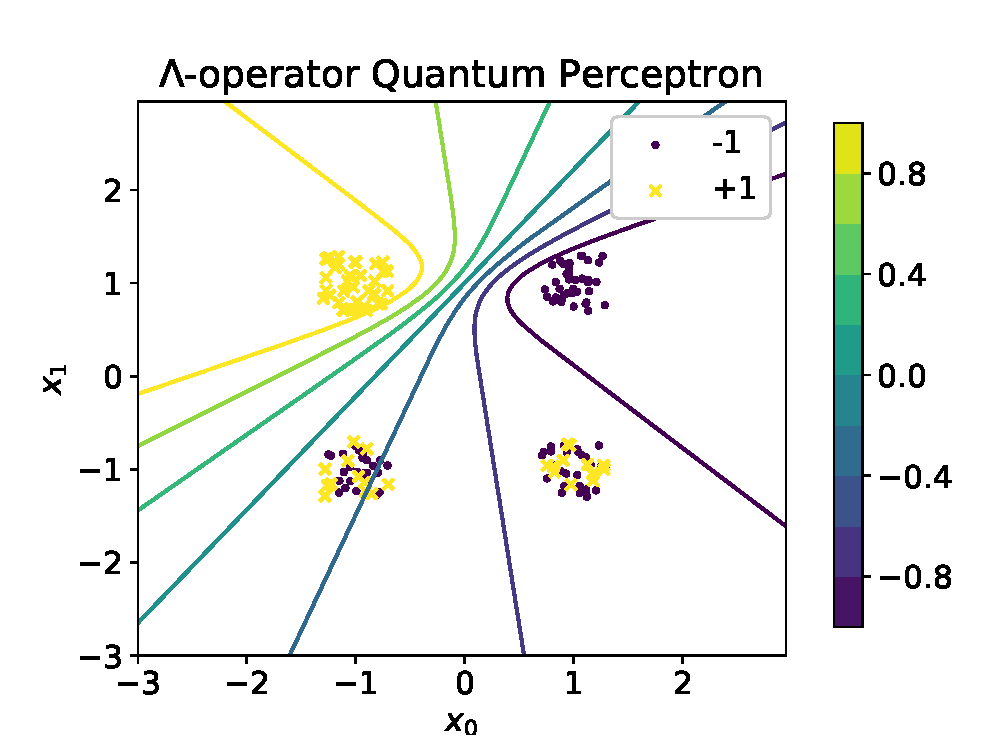
\includegraphics[width=1\linewidth]{figures/chapter3/amin.eps}
    \caption{The $\Lambda$-operator perceptron has $\text{MSE}(\Lambda) \approx 0.111$ which is higher than the $\text{MSE}(quantum) \approx 0.106$ but still lower than $\text{MSE}(classical) \approx 0.154$. We can attribute this difference in performance to the fact that the model cannot assign the same uncertainty to the two bottom data points. The point $(1,-1)$ has an expected value of $\mathbb{E}[y|\mathbf{x};\mathbf{w}]_p\approx-0.8$ while the point $(-1,-1)$ has an expected value of $\mathbb{E}[y|\mathbf{x};\mathbf{w}]_p\approx -0.4$. The $\Lambda$-operator perceptron is similar to the magnetization perceptron in this regard. The quantum perceptron assigned both these points an equal probability as desired, since both points have to same uncertainty.}
    \label{fig:amin}
\end{figure}

\section{Note on Quantum Computing}

Modern quantum computing architectures leave a lot to be desired, but are capable of performing a calculations coherently on small systems. Integrating quantum computing into this thesis would be a considerable amount of work that would differ conceptually a lot from the previous sections, which is why a deep analysis is not presented here. Instead, we discuss the outlines of some ideas that might be interesting for future work.\newline

\noindent The learned density matrix matrix of the quantum perceptron is a mixed state, which is difficult to prepare on a quantum computer, which is designed to work on pure states. But we can use a trick: we know that tracing out subsystems of entangled states can give mixed states. In fact, one can show that for any mixed state $\rho_A$ there exists a pure density matrix $\rho = \ketbra{\phi_{AR}}{\phi_{AR}}$ such that $\Tr_B (\rho) = \rho_A$ with $\ket{\phi_{AR}} \in \mathcal{H_A}\otimes\mathcal{H}_R$. The system $\mathcal{H}_R$ is a fictitious system known as the reference system. Finding the pure density matrix $\rho$ belonging to a mixed state is a process known as purification \cite{Nielsen2011}. Consider the pure state $\ket{\phi_{AR}}$, which can be decomposed into a linear combination of tensorproduct states (see Appendix \ref{sec:tens_prod}),
\begin{equation}
    \ket{\phi_{AR}} = \sum_{jk} a_{jk} \ket{j}\ket{k} 
    \label{eq:phi_general},
\end{equation}
where $a_{jk}\in \mathbb{C}$ so that $\braket{\phi_{AR}}{\phi_{AR}}=1$. With singular value decomposition we can write the matrix $a_{jk} = u_{ji}d_{ii}v_{ik}$,
\begin{equation*}
    \ket{\phi_{AR}} = \sum_{ijk} u_{ji}d_{ii}v_{ik} \ket{j}\ket{k}.
\end{equation*}
Define $ \ket{\psi^A_i} \equiv \sum_j u_{ji} \ket{j}$, $ \ket{\psi^R_i} \equiv \sum_k v_{ik} \ket{k}$ and $\sqrt{p_i} \equiv d_{ii}$, which gives
\begin{equation*}
    \ket{\phi_{AR}} = \sum_i \sqrt{p_i} \ket{\psi^A_i}\ket{\psi^R_i},
\end{equation*}
with $p_i\in \mathbb{R}_+$. This is called the Schmidt decomposition. We can write the reduced density matrix as
\begin{align*}
    \Tr_R(\ketbra{\phi_{AR}}{\phi_{AR}}) &= \sum_{ij} \sqrt{p_i p_j} \ket{\psi^A_i}\bra{\psi^A_j} \Tr_R(\ket{\psi^R_i}\bra{\psi^R_j})\\
    &= \sum_{ij} \sqrt{p_i p_j} \ket{\psi^A_i}\bra{\psi^A_j}\delta_{ij}\\
    &= \sum_i p_i \ketbra{\psi^A_i}{\psi^A_i} = \rho_A.
\end{align*}
$\ket{\phi_{AR}}$ is known as the purification of $\rho_A$. The purification scheme shows us that we can measure an effective mixed system by looking at the subsystem of a larger pure system. This means that we can simulate the quantum perceptron, which is a mixed state, on a quantum computer, such as the IBM Q Experience \cite{Qiskit}.\newline

\noindent Additionally, researchers affiliated with Xanadu, a Canadian photonic quantum computing company, have developed a Python framework that enables automatic differentiation through quantum circuit called PennyLane \cite{Bergholm2018, Schuld2019b}. This would obviate the usage of a classical computer to calculate gradients, although updating parameters would still require a classical computer. At the moment, we are investigating the possibilities of integrating the quantum log-likelihood with PennyLane. The code and research for this project can be found on Github \cite{WiersemaGit2019b}.

\section{Conclusion}

We extended the classical likelihood to a quantum log-likelihood and constructed a quantum perceptron from density matrices. The resulting algorithm is more resistant to noisy data when learning and takes this noisiness into account when predicting. This is due to the fact that there is a cost for flipped output labels in the quantum log-likelihood. For toy data sets we observed that the quantum perceptron is better at assigning probability to noisy samples, which resulted in improved performance. We focused on the analysis of possible separation boundaries for the model, to better understand what problems could be learned. \newline

\noindent We have not only considered binary classification. The quantum perceptron could be extended to multiclass regression for $C>2$ classes by considering the fundamental $\text{SU}(C)$ representations instead of the Pauli matrices. A caveat of our model is that in order to get better results than a classical perceptron, we require multiple copies of a sample $\mathbf{x}$ with conflicting labels $y$ to be present in the data. If this is not the case, our model reduces to logistic regression. By introducing a continuous similarity measure between samples that replaces the binary $b(\mathbf{x})$ statistic, we showed that non-discrete data could be learned while retaining the interesting boundaries of the quantum perceptron. Additionally, we have also shown that an entangled perceptron can be constructed with two qubits, and that an extension to $n$ qudits is trivial as long as we trace out $n-1$ qudits so that we can use the quantum log-likelihood. However, with the current construction, entangling more qubits does not give a more complex model, it simply increases the number of parameters that determine the shape of the quadric separation boundary. \newline

\noindent The quantum perceptron also provides a good starting point for constructing other physically-inspired models. Firstly, we looked into a possible classical analogue, inspired by paramagnetic materials. Even though this model had some qualitative similarities with the quantum perceptron, the current construction we came up with lacked some elegance. Secondly, we showed that physical constraints pose no significant limitation for our model. By tuning the transverse fields of a two qubit system, we were able to learn the XOR problem. This shows that we do not require all degrees of freedom that the original entangled perceptron has access to. Finally, we briefly explored the relation with Amin's quantum boltzmann machine, and outlined the possibilities for integrating quantum computing with our research.
